\documentclass{article}
\usepackage{listings}
\usepackage{minted}
\usepackage{lipsum}
\usepackage[a4paper, bindingoffset=0.2in,margin=1.2in]{geometry}
\usepackage{float}
\usepackage{amsmath}
\usepackage{hanging}
%\usepackage{xcolor}
\usepackage{textcomp}
\usepackage{tikz}
\usetikzlibrary{calc}
\usepackage{graphicx}
\usepackage{setspace}
\usepackage{subcaption}
\usepackage[utf8]{inputenc}
%\graphicspath{ {c:/Users/User/Documents/thesis/Thesis/thesisimages/} }

\graphicspath{ {./thesisimages/} }
%\usepackage{fontspec}
%\setmainfont{Minion Pro}

\begin{document}

\begin{titlepage}

\begin{tikzpicture}[overlay,remember picture]
    \draw [line width=1pt,rounded corners=0pt,
        ]
        ($ (current page.north west) + (1.6cm,-1.6cm) $)
        rectangle
        ($ (current page.south east) + (-1.6cm,1.6cm) $);
\end{tikzpicture}

    \begin{center} 
	\Large
        \vspace*{1cm}
        
        \textbf{ Integrated Deep Learning and Bayesian Classification for Prioritization of Functional Genes in Next-Generation Sequencing Data }
        
        \vspace{0.5cm}
        %subtitle here
        
        \vspace{1.0cm}
        
        \textbf{Chan Khai Ern, Edwin}
        
\vspace{9.0cm}
        \normalsize
       A thesis submitted to the \\
Department of Biochemistry \\
National University of Singapore \\
in partial fulfilment for the \\
Degree of Bachelor of Science with \\Honours
in
Life Sciences\\

        
        \vspace{1.5cm}
        
        
        Life Sciences Honours Cohort \\
        AY2015/2016 S1\\
       
        
    \end{center}
\end{titlepage}
\newpage\null\thispagestyle{empty}\newpage
\newpage
\pagenumbering{Roman} 
\doublespace
\large
\vspace*{50px}

%\vspace{50pt}

\begin{center}
\textbf{DECLARATION}\\[\baselineskip]
I hereby declare that this thesis is my original work and it has been written by me in its entirety. I have duly acknowledged all the sources of information which have been used in the thesis.\\[\baselineskip]
This thesis has also not been submitted for any degree in any university previously.\\[3\baselineskip]
\begin{center}
\line(1,0){150}
\end{center}
Chan Khai Ern Edwin\\
04 April 2017
\end{center}
\newpage
\section*{Acknowledgements}
\newpage
\section*{Table of Contents}
\small
\tableofcontents
\newpage
\doublespace
\normalsize
\pagenumbering{arabic} 
\section*{Abstract}
The advent of next-generation sequencing technology has enabled large-scale interrogation of the genome to identify variants in patient samples. The accurate identification of functional variants can provide critical insights into the disease process to guide diagnosis and treatment. However, the use of clinical genomics remains limited as (i) the accurate identification of variants remains suboptimal, and (ii) the large number of variants identified may be difficult to interpret without a systematic approach of ranking by functional importance.\\\\
Here, we describe the development of a deep learning neural network to improve the accuracy of variant-calling, and a Bayesian classification method for the probabilistic ranking of functionally relevant genes. We show that an optimised neural network can call variants more accurately than single variant callers or concordant callers, with F1 score improvements of 6 percent in simulated datasets and 4.5 percent in real datasets over the best concordant methods. Following the identification of high confidence variants, we further demonstrate that a Bayesian classification system can rank functionally relevant genes in a Diffuse Large B-Cell Lymphoma (DLBCL) patient sample.\\\\
We propose that the combined use of deep learning and Bayesian network analysis could be extended to build an analytical pipeline for clinical use to augment diagnosis and treatment of diseases by identifying high-confidence variants and ranking them systematically.
\newpage
\section{Introduction}
\subsection{Next Generation Sequencing (NGS) for Clinical Genomics}
There has been a growing interest in using a patient's genome to guide the diagnosis and treatment of diseases (Rehm, 2017; Angrist, 2016), based on the fundamental intuition that variants and mutations in the genome alter gene functions that drive the initiation and progression of the disease. In oncology, for example, identification of the key driver mutations has been shown to be useful in stratifying cancer subtypes (Stratton, Campbell \& Futreal, 2009), and identifying mutations for targeted therapy (Janitz, 2011). Furthermore, the development of next generation sequencing (NGS) technologies has dramatically reduced sequencing costs (Metzker, 2010; Mardis, 2008), enabling the adoption of genomic sequencing in clinical labs.\\\\ 
Although clinical genomics holds great promise, there are still two critical issues that limit its use in a clinical setting. Firstly, it is often difficult to obtain high-confidence variant calls from sequencing data, and secondly, the large number of variant calls for patient samples makes interpretation difficult for clinical decision-making.
\subsection{Variant Calling of NGS Data}
In variant calling, genomic DNA is fragmented, and the short reads are sequenced in a massively parallel manner using next generation sequencing technologies such as sequencing by synthesis. These reads are aligned to a reference genome, and variations in the DNA sequence, such as single nucleotide variants (SNVs) and insertions/deletions (indels) are identified by comparing the different reads aligned to the reference genome (Figure 1).
\begin{figure}[H]
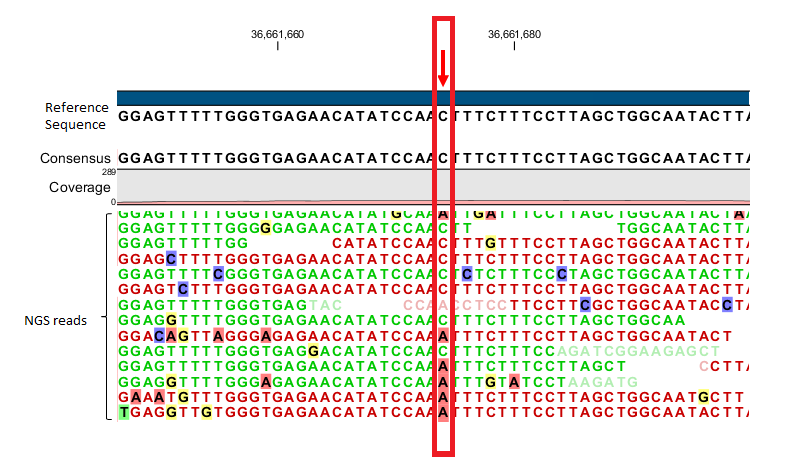
\includegraphics[width=\textwidth]{ngsreads.png}
\centering
\caption{ \textbf{Illustration of Variant Calling Pileup}. Due to noise and errors in sequencing and read mapping, it can be difficult to call variants accurately. At the position of interest, there seems to be a possible mutation from the original base of Cytosine to the base Adenine, but not all reads agree with this mutation call. Figure adapted from CLC Genomics Workbench 9.5, Figure 29.8.}
\end{figure}
Variant calling with NGS data primarily involves the use of various statistical and algorithmic methods to identify variants in the genome (Nielson et al., 2011). These variants represent the deviations and differences between the genome of interest and a reference human genome. This analysis is non-trivial as each variant call requires the integration of multiple sequence reads (e.g. millions of reads) that contain experimental noise and errors (Zook et al., 2014). The calling of variants can be further complicated by errors in mapping the reads to a reference genome.\\\\
To account for these errors, variant callers employ a variety of algorithms and statistical models to determine the existence and type of variation/mutation (Zook et al., 2014; Davey et al., 2011). Because of the differences in assumptions and models employed by different variant callers, certain calling algorithms are more sensitive and accurate in calling specific classes of variants but do not perform well in calling other variant types (O'Rawe et al., 2013). To address these problems, ongoing efforts have focused on improving current variant calling algorithms, including optimisation of variant calling for different classes of mutations, as well as the reduction in the number of false positive calls (Mohiyuddin et al., 2015; Gézsi et al., 2015).\\\\ 
Despite the variety of approaches used for identifying variants and mutations,  the accuracy and precision of single variant callers remain suboptimal (Cornish and Guda, 2015; O'Rawe et al., 2013). Each variant caller can differ greatly in accuracy depending on the type of sequencing methodology and the statistical algorithm used (Figure 2), making it difficult to identify true high-confidence variant calls.
\begin{figure}[H]
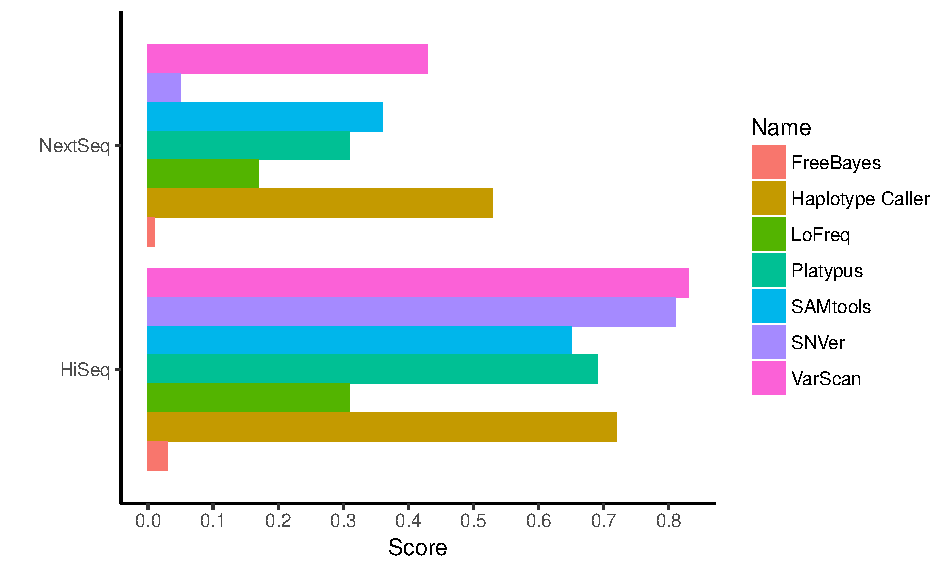
\includegraphics[width=0.8\textwidth]{f1scorerealdatasets_v2.pdf}
\centering
\caption{\textbf{Performance of Variant Calling Tools on Patient Data using the HiSeq and NextSeq Illumina Sequencing Platforms }. The F1 score indicates how well a caller can predict true positives (See Appendix 5.3 for more details). Notably, the F1 score for the same variant calling tool can differ greatly. Figure adapted from Sandmann et al. (2017)}
\end{figure}
\subsection{Ensemble Methods for Improving the Accuracy of Variant Calling} 
While it is clear that single variant callers may not perform well across a variety of variant classes, the combination or ensemble of several callers can be used to augment the accuracy of variant callers beyond what can be achieved with a single caller. By aggregating the calls from each different variant caller, the relatively weak prediction calls from each caller can be combined to provide a better aggregate prediction for a variant call. 

One simple approach to aggregating variant calls is by concordance, where the likelihood of an accurate call depends on multiple variant callers identifying the same variant or mutation (Lam et al., 2012; Wei et al., 2011). While straightforward and intuitive, the recall rates of such a tool is poor with a high number of false negative calls. This is because a high concordance of variant calls will reciprocally decrease the number of true variants calls that are identified by specific variant callers (O'Rawe et al., 2013).

Beyond concordance, supervised machine learning approaches have been used to combine the calls from different variant callers to improve calling accuracy. In these methods, machine learning algorithms have been used to predict the accuracy of a variant call by integrating different features of each variant call (e.g. variant frequencies, mapping quality). For example, the support vector machine (SVM) algorithm was used successfully to improve the accuracy of variant calls (Gézsi et al., 2015) over concordance-based methods. 

Recent advances in machine learning, in particular, deep learning neural networks, have increased the accuracy of predictions from complex multi-modal data (Schmidhuber, 2015) beyond traditional algorithms such as SVM and Random Forests. The ability of deep learning networks to learn from complex high-dimensional data suggests that they may be useful in improving the accuracy of high-confidence variant calls derived from the complex features from each variant caller. 
\subsection{Deep Learning for Improving the Accuracy of Variant Calling} 
Deep learning is a machine learning approach based on artificial neural networks (LeCun et al., 2015) that are built on artificial neurons. Each artificial neuron is analogous to a biological neuron where weighted input signals are integrated to produce an output once the signals cross a threshold for activation (Figure 3).  
\begin{figure}[H]
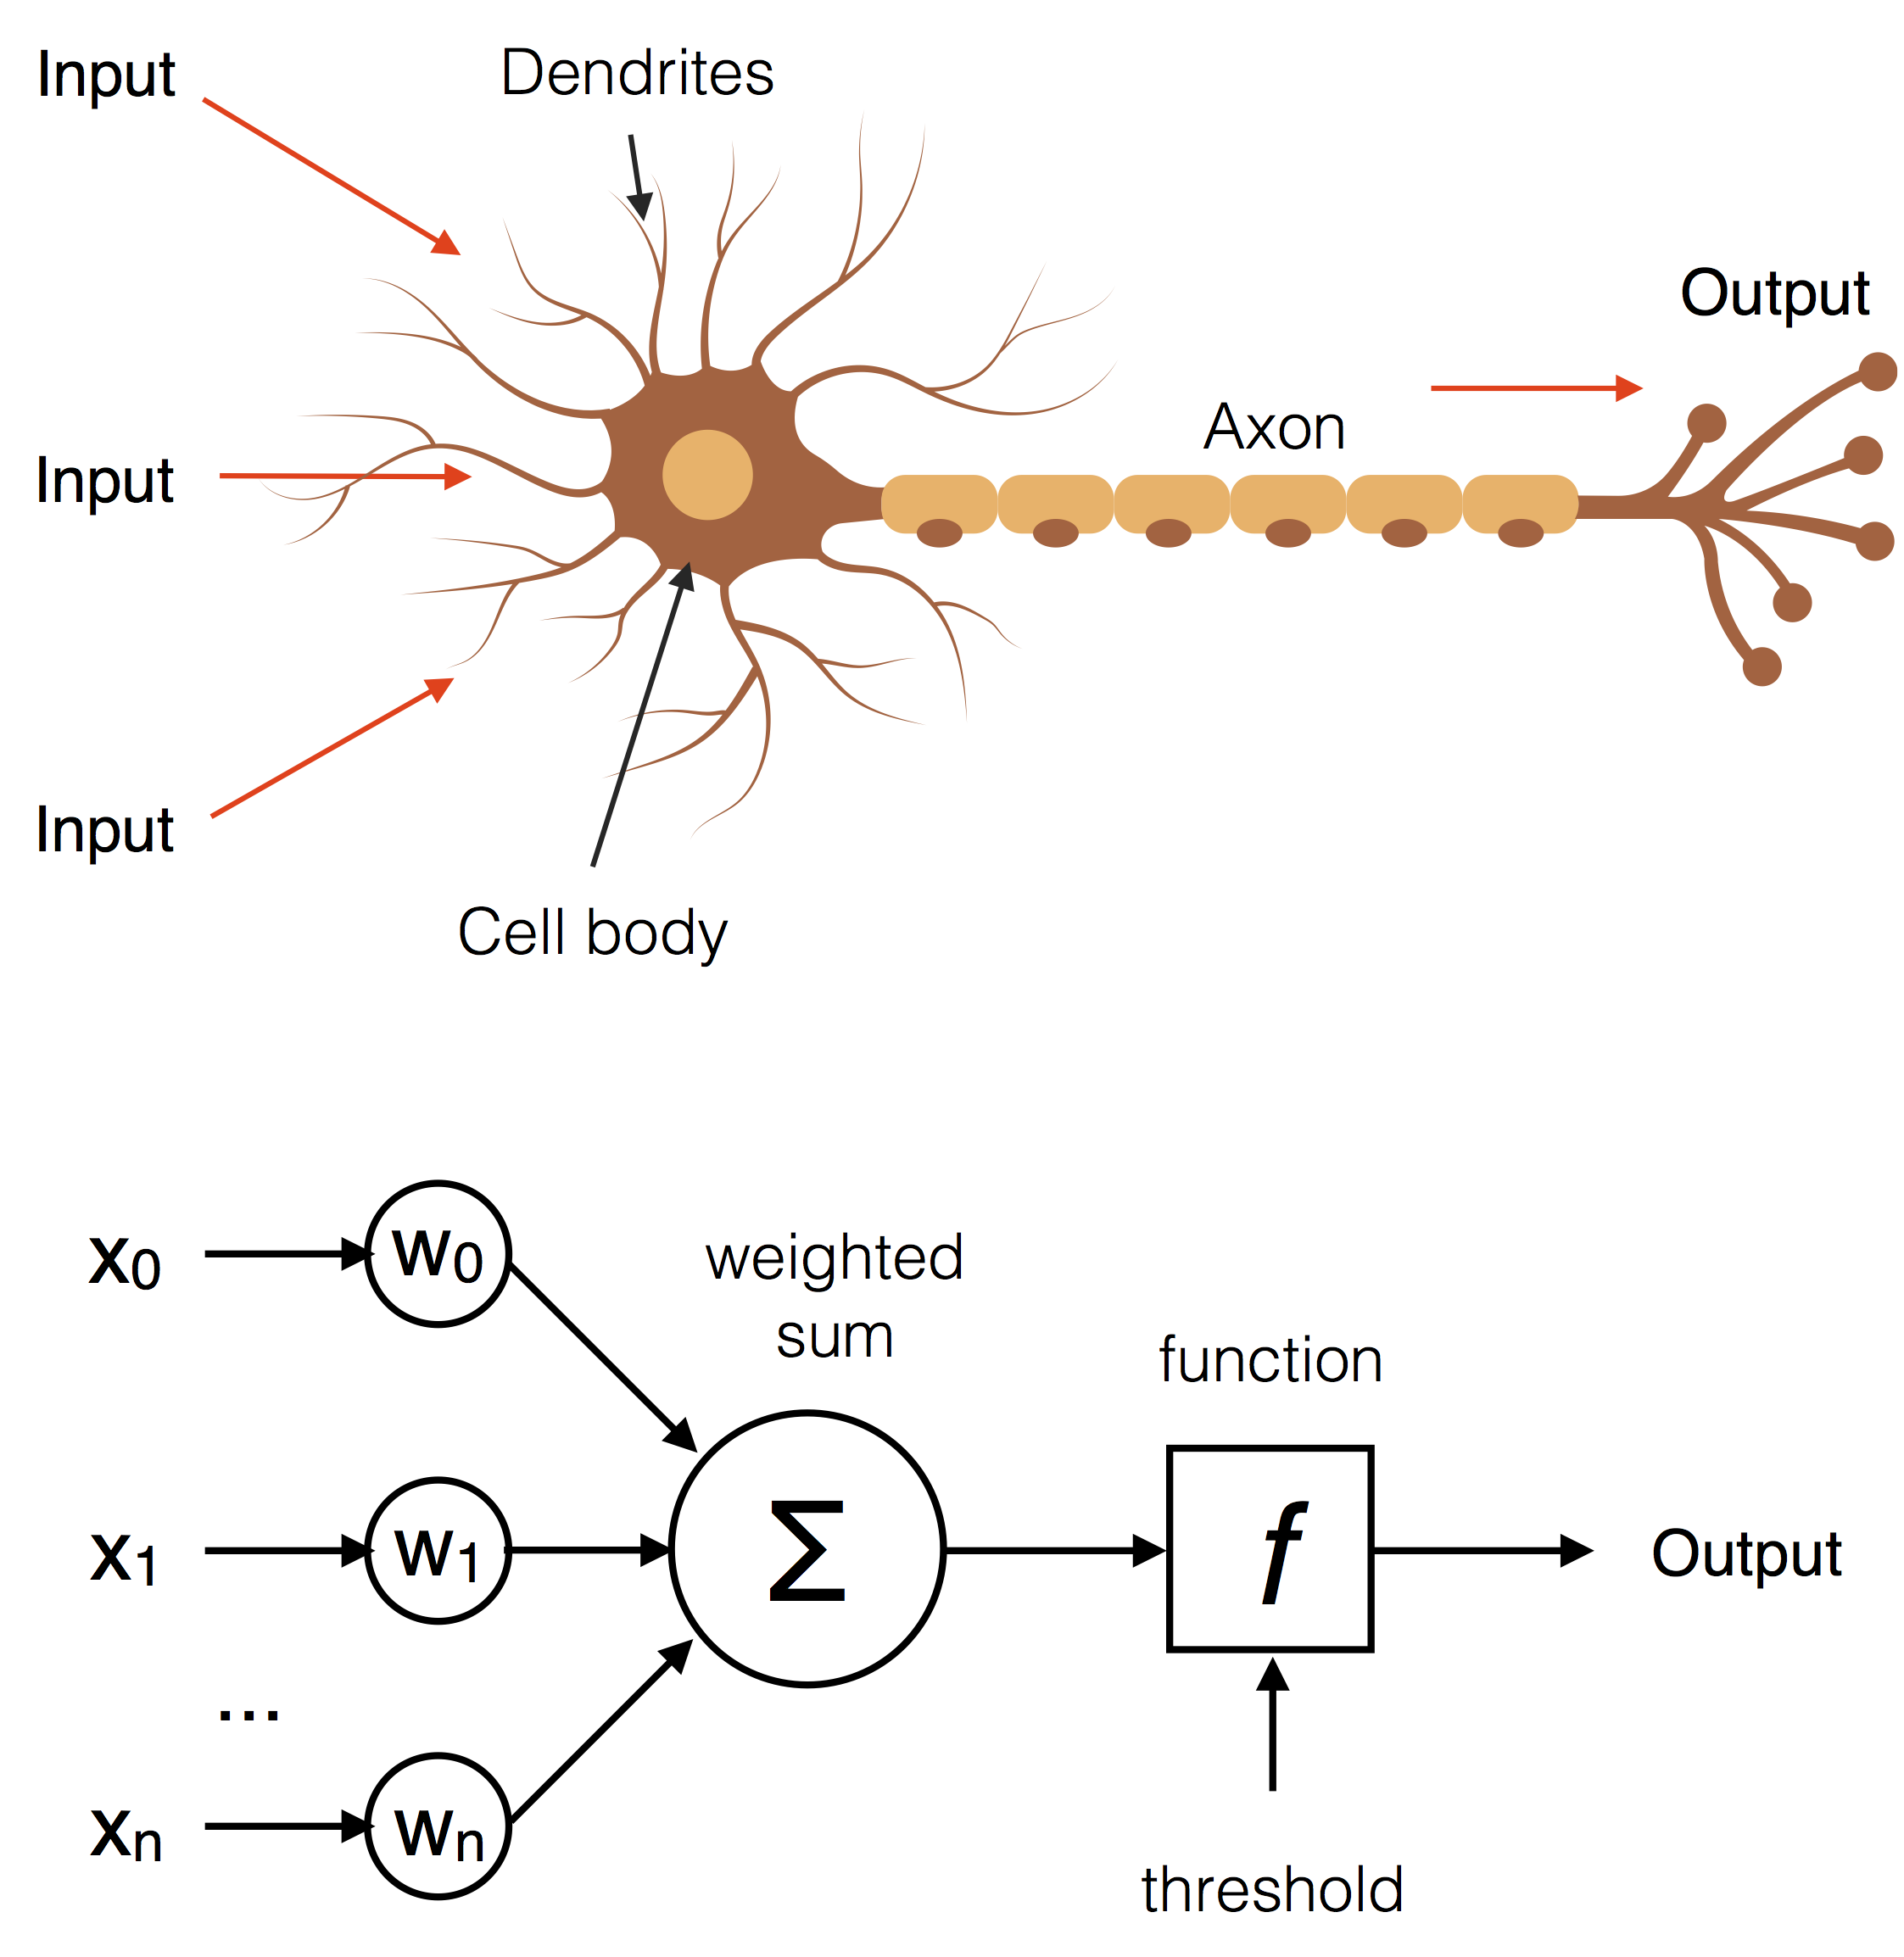
\includegraphics[width=0.7\textwidth]{neuron.png}
\centering
\caption{\textbf{Artificial Neurons as Building Blocks of Neural Networks}}
\end{figure}
In a deep learning network, the artificial neurons are connected in layers, comprising an input layer, an output layer, and a variable number of intermediate hidden layers (Figure 4). Here, the outputs of the neurons in one layer are connected to the inputs of next layer of neurons, with the weights of the connections determining the strength of signal propagation from one neuron to another.

\begin{figure}[H]
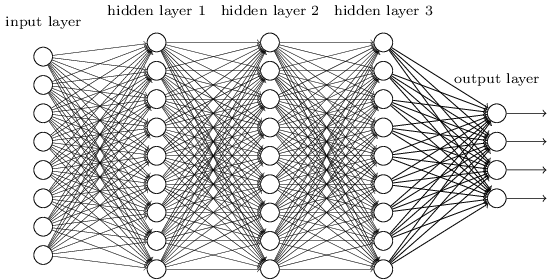
\includegraphics[width=\textwidth]{neuralnet.png}
\centering
\caption{\textbf{Sample Neural Network with Five Layers, Including Three Hidden Layers}. This diagram represents a densely connected neural network, where each node is connected to every node of the preceding and subsequent layers.}
\end{figure}
Deep learning networks can be trained by providing labelled data, where features of the dataset are fed into the input layer to produce the output prediction. By comparing the output to the actual labels, the network can be trained by adjusting the weights that determine the propagation of a signal from one neuron to the next. In this way, a trained neural network can predict the output when given new data (for a more detailed explanation, see Appendix 5.1).

Because deep learning networks contain multiple layers, they can learn different features in a hierarchical manner. This allows the network to solve complex non-linear decision boundary problems, including drug molecule solubility (Lusci et al., 2013), facial recognition (Sun et al., 2014) and even predicting the best move in the Japanese board game, Go (Silver et al., 2016). Given this ability to learn from complex features, deep learning networks provide a possible approach to improve the prediction high-confidence variant calls from an ensemble of different variant calling algorithms.
 
\subsection{Prioritisation of Variants with Bayesian Networks}
Once high-confidence variant calls can be established, there remains the second problem of identifying the functional importance of each variant/mutation, given that there are multiple variants in a typical genome (Shen et al., 2013). The ability to systematically prioritise and rank clinically significant variants would allow clinicians to focus their attention on relevant candidate mutations that can guide decision-making on diagnosis and treatment.

 The problem of prioritisation of genetic variants and mutations arises from the multiplicity and complexity of data sources that can be utilised to determine the clinical and functional relevance of a variant or mutation in a gene (Moreau \& Tranchevent, 2012). Several approaches have been used, including characterising variants and their phenotypes in clinical cases, and determining if a variant/mutation will alter protein function based on amino acid changes in conserved regions. Although these functional annotations of variants and mutations can be performed with tools such as ANNOVAR (Wang, Li, \& Hakonarson, 2010), the fundamental problem of integrating the information in a systematic manner remains. 
 
 One possible approach to addressing this problem is by using Bayesian networks to probabilistically integrate diverse information sources to predict the likelihood of an outcome. This approach has been successfully used in solving a variety of decision making problems (Pourret et al.,2008; Jensen et al., 1996), including medical treatment decision making (Windecker et al., 2014), ecological studies (Johnson et al., 2014) and predictive epidemiology (Su et al., 2014).
 
 In a Bayesian network, the probabilities of different events can be linked so that the final likelihood of an outcome can be evaluated. An example of a simple Bayesian network is shown in Figure 5. Here, the likelihood of the outcome, which is rain, is dependent on the probabilities of thunder, cloudy day and the weather forecast. The probabilities of the variables can be used to update the final likelihood of the outcome, based on the conditional probabilities of thunder, cloudy day, and weather forecast. In a similar way, the probability of a functionally important variant/mutation can be evaluated based on the conditional probabilities of the functional annotation and confidence of a true variant call.
 
\begin{figure}[H]
\centering
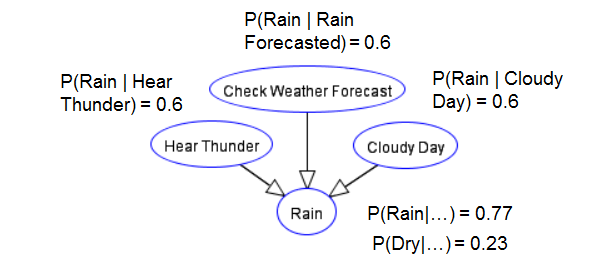
\includegraphics{samplebayesiannetwork.png}
\caption{\textbf{Sample Bayesian Network for Rain Prediction.}}
\end{figure}

One advantage of Bayesian network analysis is that it approximates how humans reason about relationships between events and outcomes - we observe events and update our probabilistic estimates of the likelihood of an outcome. Additionally, because Bayesian networks require the explicit specification of relationships between the events and the outcome, the model is transparent and can be built based on known relationships between events, based on existing knowledge.

Bayesian networks are well suited to ranking the importance of functionally important variants/mutations because the model can be built using the explicit specification of the probabilities accounting for the high confidence calls and the predicted functional effects of the variants/mutations. This explicit specification permits a better understanding of the ranking process, which is important for clinical decision-making.
\subsection{Aims and Approach}
The overall goal of this project is to address the two major issues limiting the utility of clinical genomics through the following aims:
\begin{enumerate} 
    \item To develop and validate a deep learning network model for improving the accuracy of variant calling.
    \item To develop a Bayesian network model for ranking functionally important variants/mutations from high confidence calls identified by the deep learning network.
\end{enumerate}

 We describe the development of (i) a deep learning network to identify high-confidence variant calls (focusing on SNVs and short indels) and (ii) a Bayesian network to probabilistically prioritise their functional importance. As a first step, we developed and optimised a deep learning network to identify true variants in both synthetic and real-world datasets. Following the identification of high-confidence variant calls, we built a Bayesian network ranking system based on functional annotations to prioritise mutations and used it to identify functionally important mutations in a cancer sample.
\newpage
\section{Materials and Methods}

\subsection{Overall Experimental Approach}
As a first step in the development of deep learning networks for variant calling, we  built two main computational pipelines : (i) a training pipeline for training and the optimisation of the neural network, and (ii) an analysis pipeline that uses a trained neural network to perform variant prediction and validation (Figure 6). \\\\
In the training pipeline, training datasets from synthetic and real sequencing data were used for performing the processing steps of alignment, variant calling and training of the deep learning network. Briefly, FASTQ sequence reads were first mapped to the reference genome before variant calling was performed using an ensemble of callers. The different variant callers were used to generate the feature vectors used as the input for the deep learning network. The predictions by the neural network were compared to the ground truth variant calls to train the network to predict high confidence variants.\\\\
 In the analysis pipeline, the trained optimised network from the training pipeline is then used to predict high-confidence variant calls in naive samples without ground truth variant calls. In brief, the FASTQ sequence reads are aligned and variant calling performed in a similar fashion as in the training pipeline. The feature vectors from the ensemble of callers is used to predict high confidence calls using the trained and optimised deep learning network.\\\\
 Finally, we applied the Bayesian network analysis to rank the functionally important variants/mutations from the high confidence calls identified from naive samples in the analysis pipeline.\\\\
\begin{figure}[H]
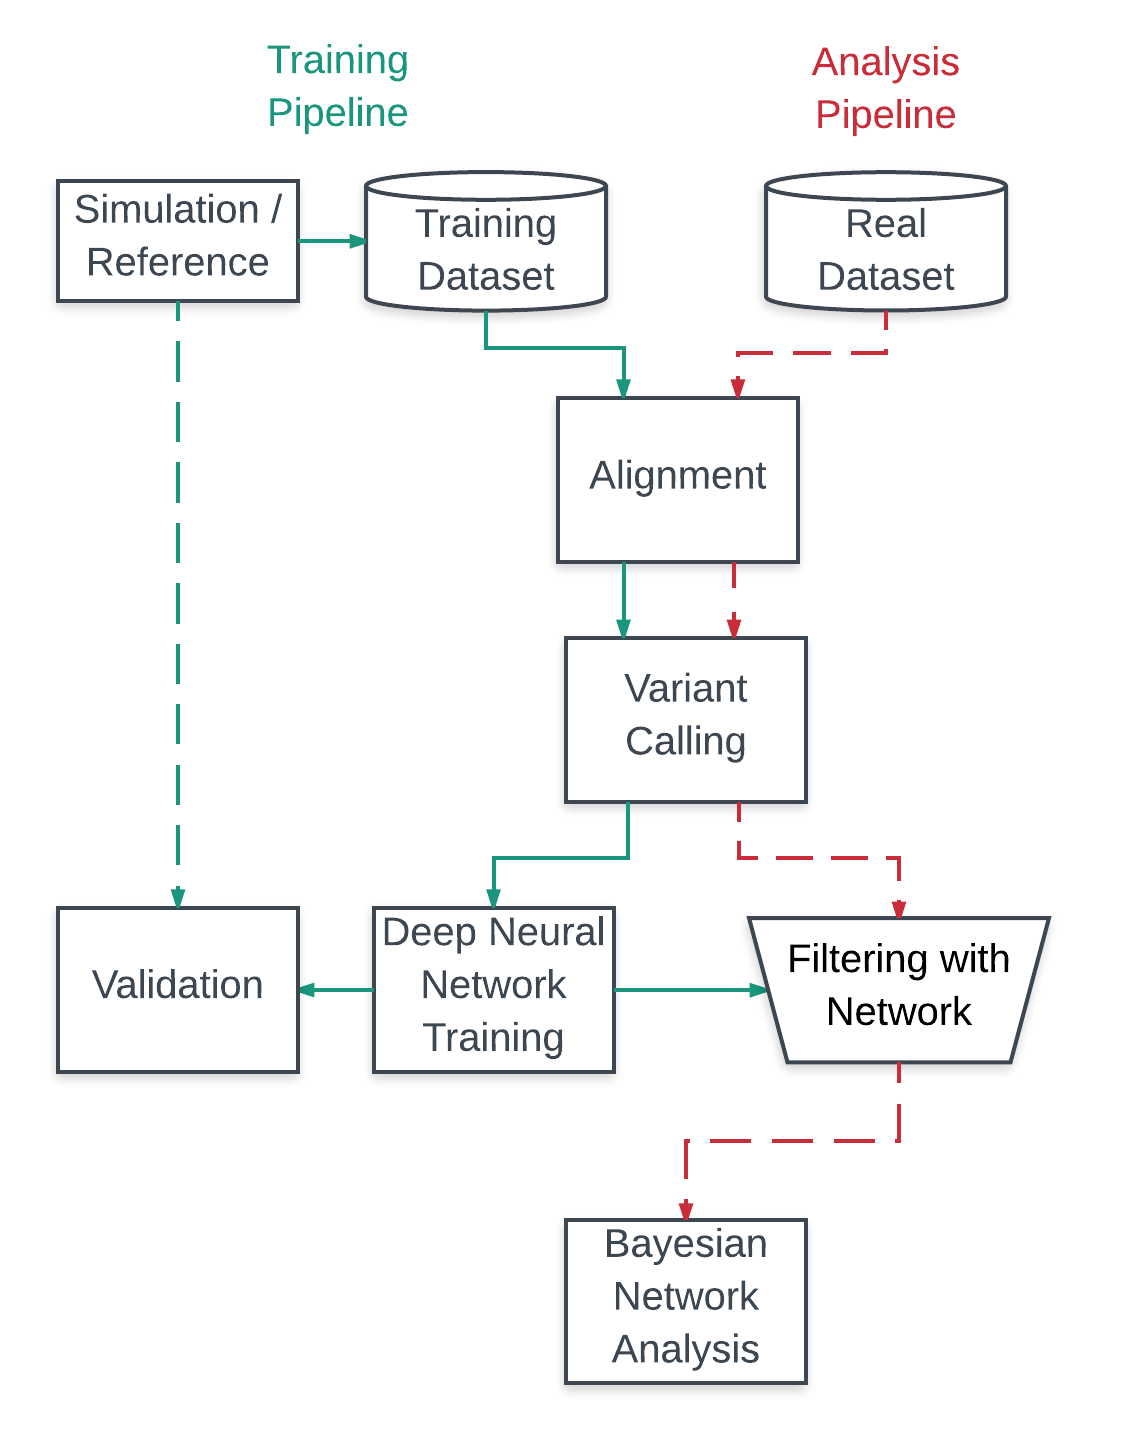
\includegraphics[width=0.8\textwidth]{trainingpathway.png}
\centering
\caption{\textbf{Overall Structure of Computational Pipelines.} The pipelines were implemented using NextFlow, a domain-specific language for workflows}
\end{figure}
\subsection{Implementation of Computational Pipelines}
\subsubsection{Workflow Management of Pipelines}
The workflows in the training and analysis pipelines were managed using NextFlow (v0.21.3.3990), a Groovy based Domain Specific Language (DSL) that provides easy management of parallel pipelines consisting of dependent tasks organised as a directed acyclic graph (Tommaso et al., 2014). Nextflow was used to manage and coordinate the different steps in the pipelines to ensure reproducibility and scalability.
\subsubsection{Preprocessing and Analysis}
The preprocessing and analytical components were implemented using Python (v2.7) (Van Rossum, 2007) and the following Python libraries: NumPy, scikit-Learn, Pomegranate and PyVCF. Briefly, NumPy (v1.11.3) was used to prepare feature vectors for deep learning training, scikit-learn (v0.18.1) was used to perform Principal Component Analysis (PCA) and Synthetic Minority Oversampling Technique (SMOTE) Methods (See Appendix 5.3 for details). PyVCF (v0.6.8) was used to parse the VCF files to facilitate the comparison of variants efficiently in O(1) time using hash-based dictionary lookups. 
\subsubsection{Implementation of Deep Learning Networks}
Deep learning networks were implemented using the Keras library (v1.1.1) with a TensorFlow backend (v0.11.0). TensorFlow, from Google (Abadi et al., 2015), was used for better network training performance due to its distributed computation and queue management system. For each of the network architectures, we used the LeakyReLU activation function. The LeakyReLU is a refinement of the ReLU activation function which minimises the "dying ReLU" problem, and both are well-documented activation functions that have been shown to work well in deep neural networks (Anthimopoulos et al., 2016; LeCun, Bengio \& Hinton, 2015; Maas, Hannun \& Ng, 2013). Additionally, dropout filters were used to prevent overfitting of data (Srivastava et al., 2014).\\\\
The code used to generate the feature vectors and train the neural network can be found in Relevant Code -- Section 7.1 and 7.2 respectively. Details on the algorithms used in deep learning can be found in Appendix 5.1.
\subsubsection{Bayesian Network Ranking of Mutations}
For the Bayesian ranking of mutations, the high confidence calls from the deep learning network were annotated using ANNOVAR (v2015Jun17) (Wang, Li, \& Hakonarson, 2010). The annotated features for each variant were used as inputs to the Bayesian network, which was implemented using Pomegranate (v0.6.1), a Python library for Bayesian analysis. The implementation code for the Bayesian network can be found in Relevant Code -- Section 7.3.
\subsection{Simulated Datasets}
Simulated genomes enable the simulation of NGS data with ground truths to test and validate a neural network. For our simulator, we used Mason, a genome mutation software written in C++ (v2.3.1) to mutate the hg19 reference genome from UCSC (Karolchik et al., 2014). We used indel rates of 0.00002 and SNP rates of 0.00008 to generate sufficient truth variants for analysis, which comprise 229253 SNPs and 57257 indels.\\\\
After generating a ground truth model, we simulated sequence reads with error rates and ground truth variants (Figure 7). For error rates, we used published data from Schirmer et al. (2016) as the input to Mason -- the general substitution error rate was 0.0004 per base in the genome, and the insertion and deletion error rate per base were $5*10^{-6}$.
\subsection{Alignment and Variant Calling of Sequence Reads} 
The sequence reads (FASTQ) from simulated or real datasets were first aligned to the hg19 human reference genome using BWA (0.7.13) (Li, 2013) using the default settings. Following alignment, the alignment files (BAM) were used for variant calling with the following callers with their default settings: FreeBayes (v1.0.2-16); GATK Haplotype Caller (v3.7-0) and Unified Genotyper (v3.7-0); Samtools (v1.3.1); Pindel (v2.3.0) (Garrison \& Marth, 2012; McKenna et al. 2010, DePristo et al. 2011; Li H, et al., 2009; Ye et al., 2009). The overall process is shown in Figure 7.
\subsection{Feature Engineering}
In order to train a neural network, features in the form of numerical vectors must be used as an input. We subset our features into three broad sets, which are base-specific information, sequencing error and bias information features, and calling and mapping quality. 
The computation of the features was performed as described below. For an in-depth explanation of their usage and interpretation, see Appendix 5.2.\\\\
\textbf{Base Information} \\*[0.3\baselineskip]
\underline{Shannon Entropy}\\*
Shannon Entropy captures the amount of information contained in the allele sequences. It is calculated using the equation:
\begin{equation}
H(X) = -\sum_{i=1}^{n}P(x_i)\log_{2}P(x_i)
\end{equation}
where $P(x_i)$ is the prior probability of finding each base at each position. This prior probability is calculated in two ways -- over the entire genome and over a region of space around the allele (10 bases plus the length of the allele in our calculations).\\[0.3\baselineskip]
\underline{Kullback Leibler Divergence}\\
The Kullback-Leibler Divergence feature is similar to Shannon entropy, but instead, we use this to measure the informational gain from the reference to the allele sequence. The Kullback-Leibler Divergence is calculated as follows:
\begin{equation}
D_{KL}(P||Q) = -\sum_{i=1}^{n}P(x_i)\log_{2}{\frac{P(x_i)}{Q(x_i)}}
\end{equation}
where $Q(x_i)$ is the prior probability of finding each base at each position based on the genomic region around the allele, while $P(X_i)$ is the posterior probability of finding a specific base inside the allelic sequence.\\[0.3\baselineskip]
\underline{Base Quality}\\
Base quality refers to the Phred score probability that the called allele is wrong. It is given by the equation:
\[ \scalebox{1.2}{$P=10^{\frac{-Q}{10}}$} \]
Where P is the Base Quality, and Q is the probability that the allele called is wrong. This is a number computed by the sequencing machine based on the quality of the base samples provided.\\\\
\textbf{Sequencing Biases and Errors} \\[0.3\baselineskip]
\underline{GC content}\\
This feature comprises the GC content of the reference genome for at least ten bases around the mutation site.\\[0.3\baselineskip]
\underline{Longest homozygous run}\\
This feature comprises the longest similar string of bases in the reference genome, for at least ten bases around the mutation site.\\[0.3\baselineskip]
\underline{Allele Count and Allele Balance}\\
This feature is an output from Haplotype Caller and Unified Genotyper, and describes the total number of alleles contributing to a call and the balance between reference and alternate alleles reads.\\\\
\textbf{Calling and Mapping Qualities} \\*[0.3\baselineskip]
\underline{Genotype Likelihood}\\*
The genotype likelihood score provides the Phred-scaled likelihood scores of how confident the caller is in determining that it is a homozygous or heterozygous call, and is provided by all variant callers.\\*[0.3\baselineskip]
\underline{Read Depth}\\*
Mapped read depth refers to the total number of bases sequenced and aligned at a given reference base position. It is provided by all variant callers.\\[0.3\baselineskip]
\underline{Quality by Depth}\\*
Quality by depth is computed by dividing the quality score against allele depth, to obtain an average score of allele quality. This is provided by Haplotype Caller and Unified Genotyper.\\[0.3\baselineskip]
\underline{Mapping Quality}\\
Mapping quality is a score provided by the alignment method and gives the probability that a read is placed accurately. It is provided by all variant callers except Pindel.\\

\subsection{Patient Derived Xenograft Mouse Model Development and Sequencing}
A patient-derived xenograft model of diffuse large B-cell lymphoma DLBCL was performed by the Mouse Models of Human Cancer Unit (MMHCU) at the Institute of Molecular and Cell Biology (IMCB), in accordance with the approved protocols by the Institutional Review Board (IRB). In brief, a sample of the DLBCL tumour was implanted into NOD-SCID-gamma mice and serially propagated as a xenograft. The DNA from the xenograft was extracted for high-throughput sequencing using the Illumina HiSeq platform (Genotypic Technology, India). The sequence reads from the xenograft were used to validate the Bayesian network ranking of functionally important mutations. 
\newpage
\section{Results}
\subsection{Generation of Synthetic Datasets}
As a first step towards developing a deep learning network, we generated a synthetic dataset containing known truth variants as labels for supervised learning (Escalona, Rocha \& Posada, 2016). To do this, we generated a synth genome with mutations using the hg19 genome from UCSC (Karolchik et al., 2014) as a reference. The synthetic genome contains over 300,000 random mutations spread over the chromosomes (Figures 8 and 9). This genome was used to generate NGS sequence reads incorporating error profiles from the Illumina platform

\begin{figure}[H]
\centering
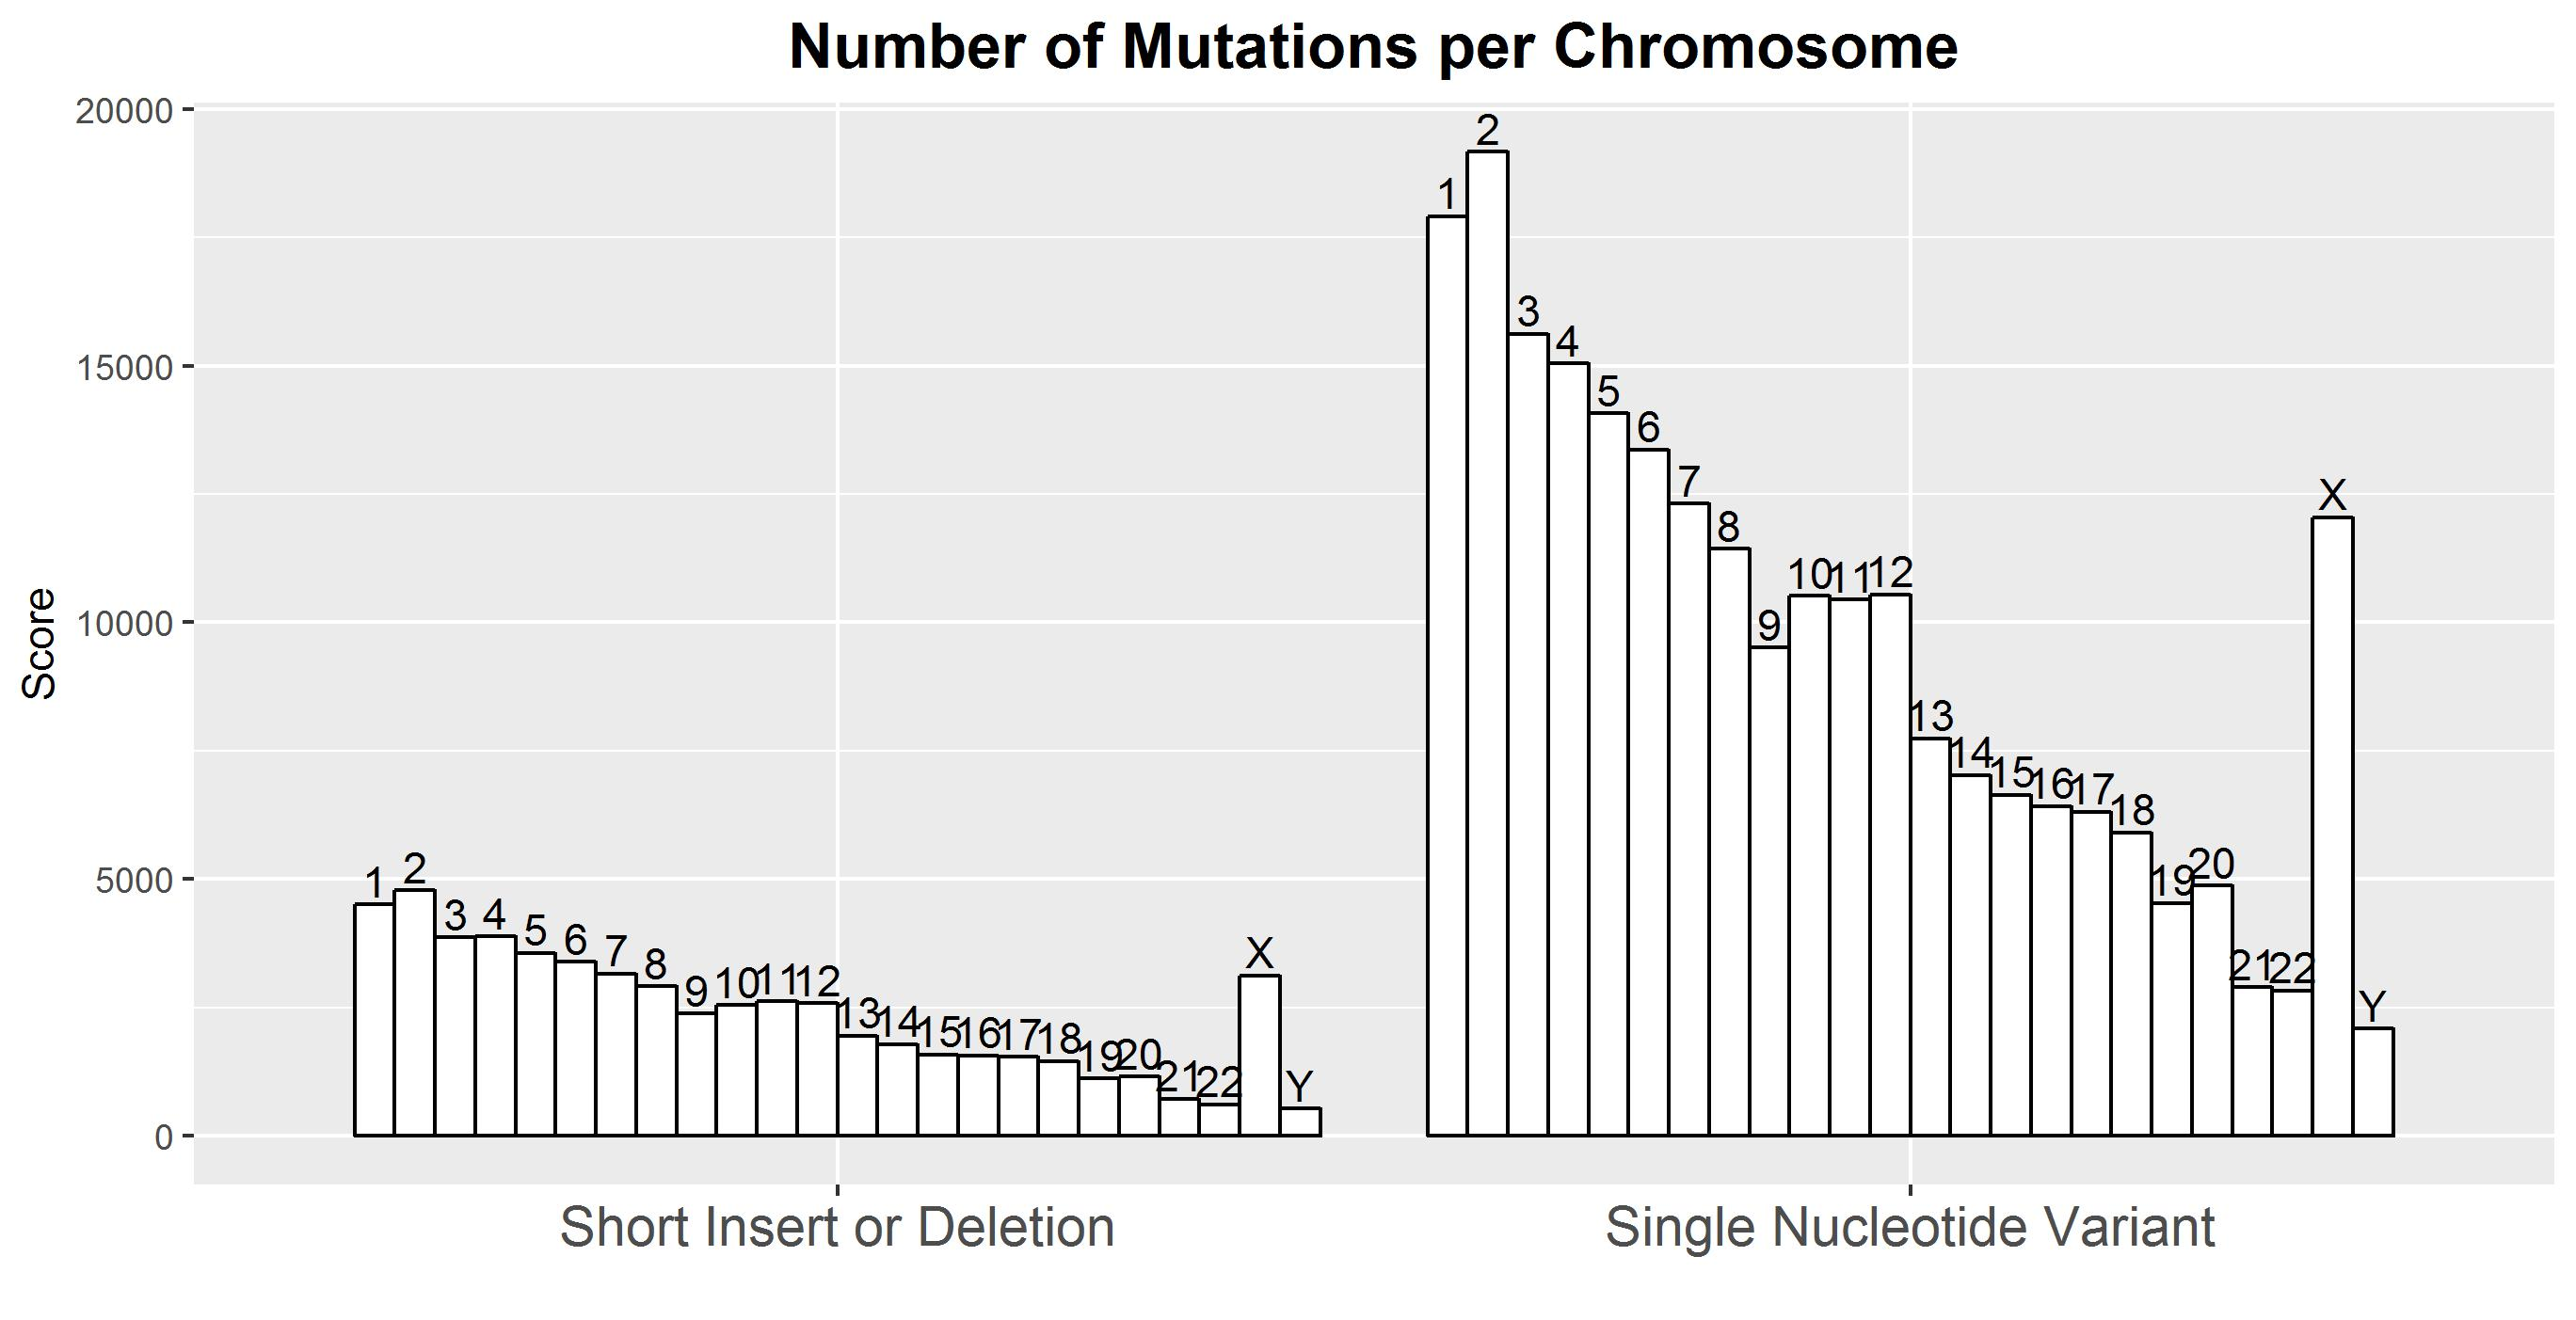
\includegraphics[width=\textwidth]{MutationInSimulatedGenome.jpg}
\caption{\textbf{Number of Ground Truth Mutations (Variants) Created in Each Chromosome}}
\end{figure}

\begin{figure}[H]
\centering
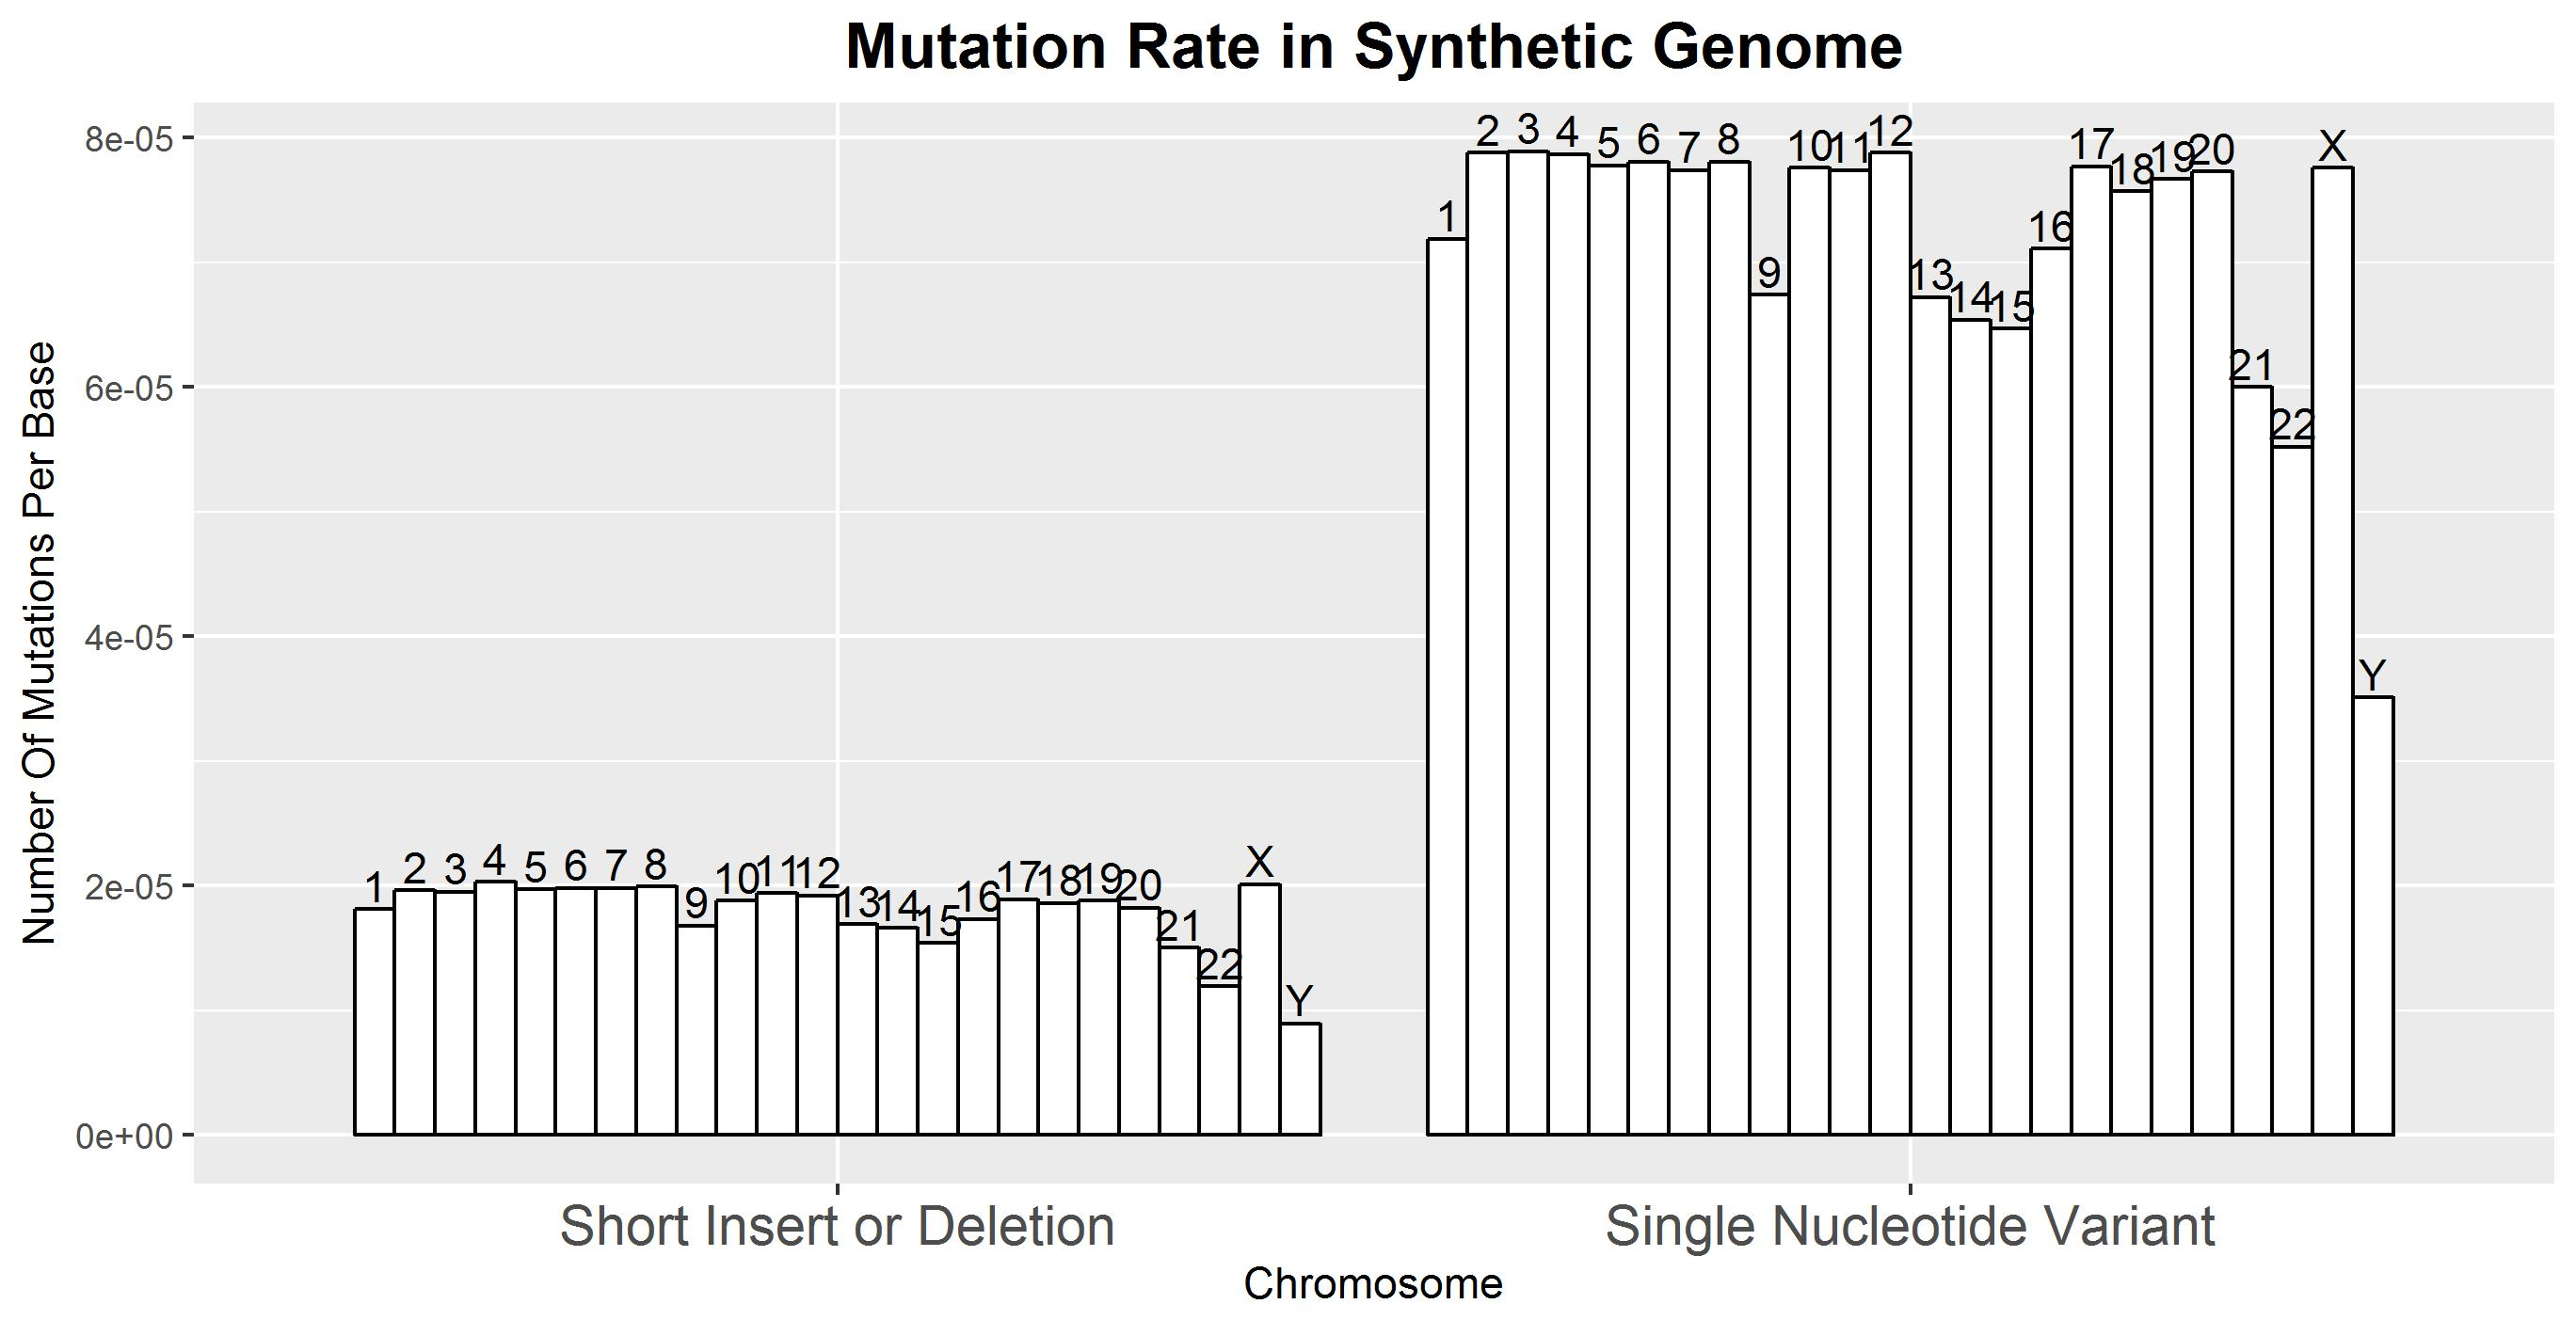
\includegraphics[width=\textwidth]{MutationRateInSimulatedGenome.jpg}
\caption{\textbf{Mutation Rate per Base in Each Chromosome}}
\end{figure}

\subsection{Feature Engineering}
Deep learning requires features to be vectorised and normalised to be used as input data. We assembled a set of 20 features, using data obtained from the variant callers themselves as well as engineering other features from the dataset. A summary of the features used in training can be found in Table 1, and a description of the full list of features can be found in Appendix 5.2.\\\\
Features were engineered based on obtaining information on the main aspects of variant calling, which includes the information contained in the sample bases (Base Quality, Entropy, Kullback–Leibler divergence, etc.), the confidence we have in the calling and alignment (Read Depth, Mapping Quality etc) and finally possible biases in the sequencing machine (Allele Balance, Allele Count, GC content).

\begin{table}[H]
\caption{\textbf{Key Features Engineered from each Caller.}}
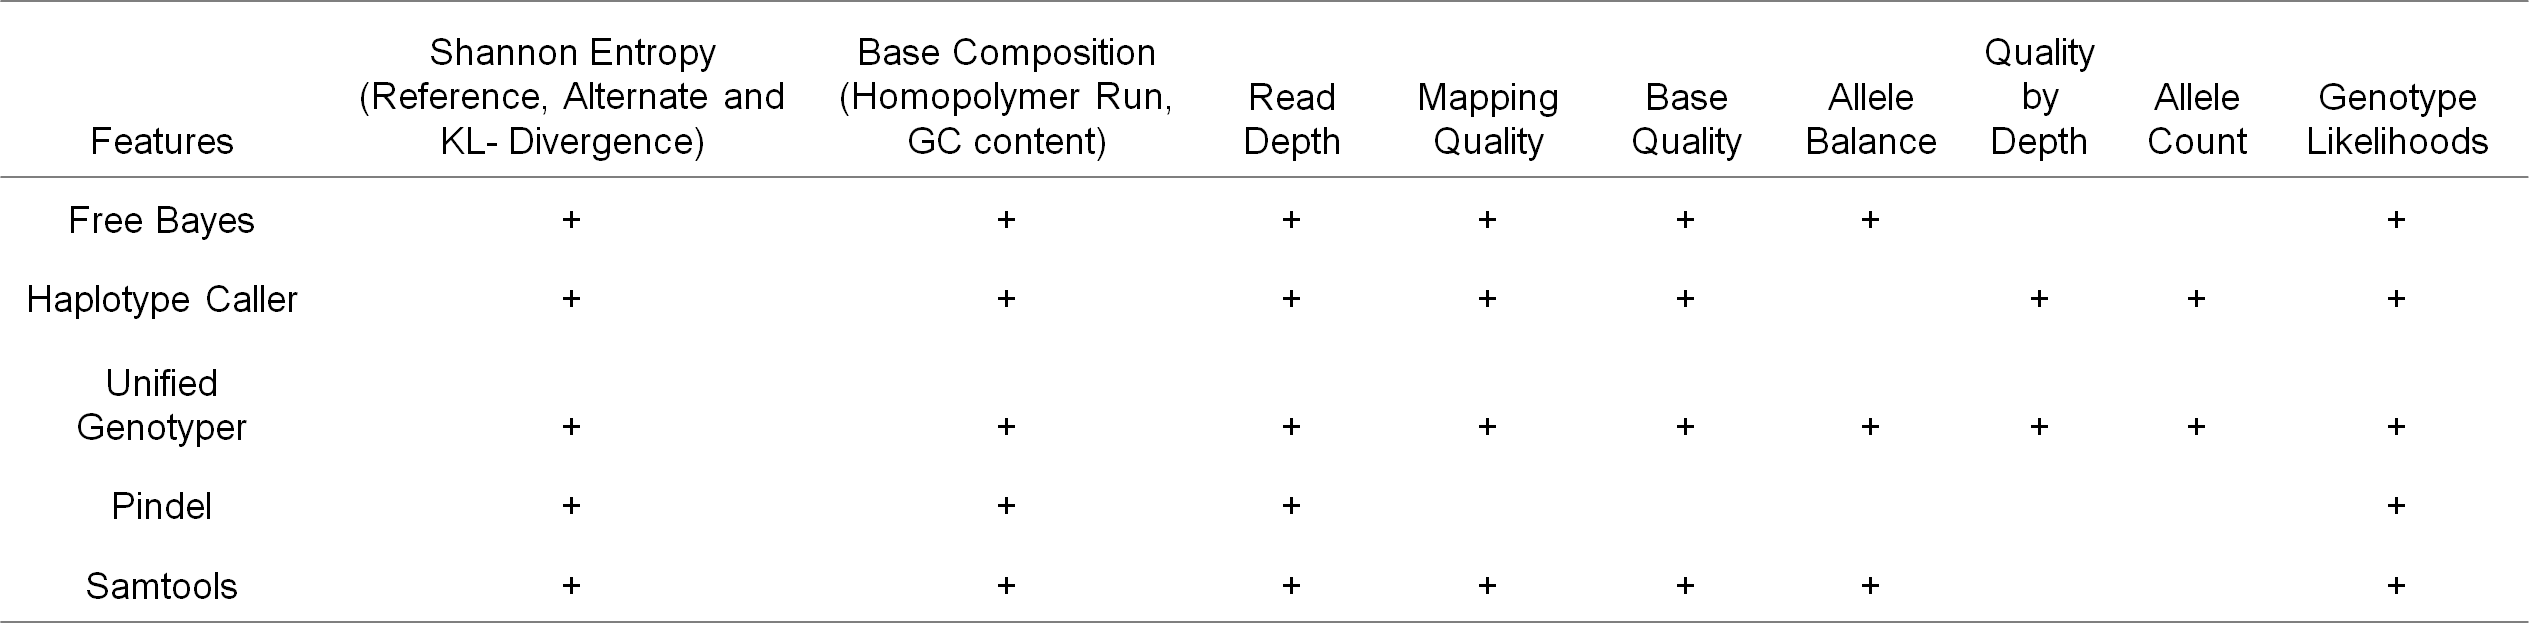
\includegraphics[width=\textwidth]{featureengineering.png}
\centering
\end{table}
\subsection{Variant Calling and Concordance}
For the training of the deep learning network, we used a mix of variant callers that use orthogonal calling and reference methodologies in order to maximise the information that the neural network can use for prediction (See Table 2).\\\\
We used two haplotype-based callers, FreeBayes (Garrison \& Marth, 2012) and GATK Haplotype Caller (McKenna et al. 2010, DePristo et al. 2011), two position based callers GATK Unified Genotyper and Samtools (Li H, et al., 2009) and finally Pindel, a pattern growth based caller (Ye et al., 2009). When we analysed the concordance rates of the callers on the synthetic dataset, we found a high number of calls were not concordant, with many calls only identified by a minority of variant callers (Figure 10).
\begin{figure}[H]
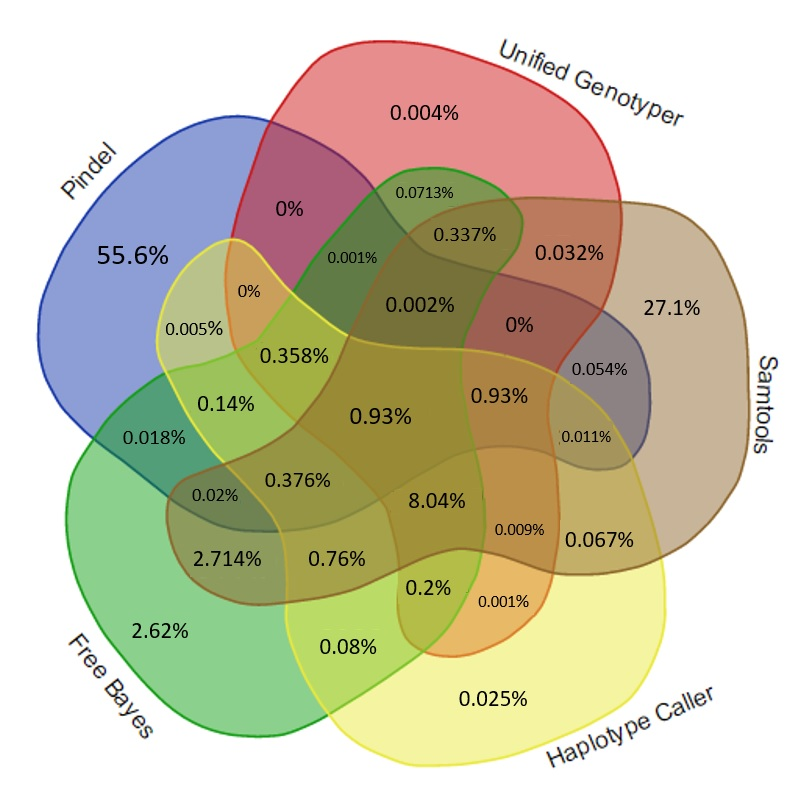
\includegraphics[width=\textwidth]{venndiagram.jpg}
\centering
\caption{\textbf{Concordance of Callers on Synthetic Dataset}}
\end{figure} 
We found that Pindel was the most discordant caller, with over 1.6 million\ (55.6\%) unique calls that are different from other calls. Samtools was also discordant, with over 800 thousand unique calls (27.1\%) that were unique from the other callers, followed by FreeBayes at 80,000 calls. These discordant calls are consistent with the different methodologies used by each variant (Table 2), leading to different calling profiles. Because of the high discordance of variant calls, identifying high-confidence calls by simple concordance is not likely to be optimal, but may be better handled by machine learning algorithms such as deep learning that can account for complex interrelationships.\\

\begin{table}[H]
\caption{\textbf{Comparison of Different Methods and Features of Variant Callers.}}
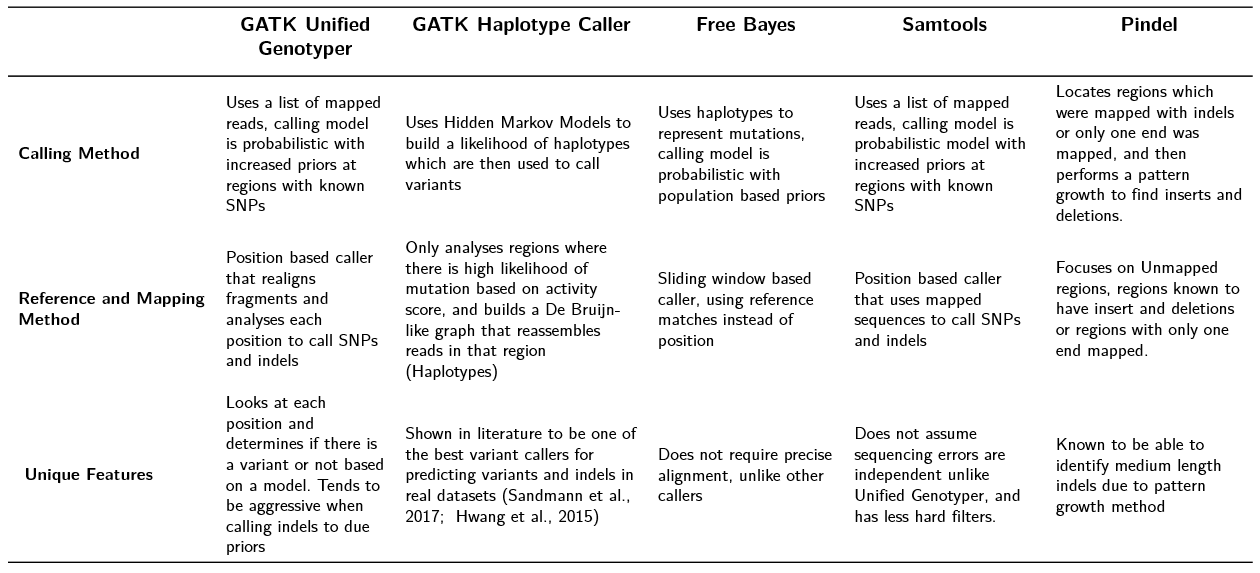
\includegraphics[width=\textwidth]{analysisofvariantcallers.png}
\centering
\end{table}

\subsection{Network Architecture}
The deep learning network can be designed using different structures that may differ in performance depending on the characteristics of the input data.  To do this, we tested out various neural network architectures to see which architecture would perform the best for our set of input features (Figure 10). In order to compare the performance of the different network architectures, we calculated the precision, recall and F1 score from the predicted variant calls in each network: (i) the precision score is defined as ratio of true positives over false positives and true positives; (ii) the recall score is the ratio of true positives over true positives and false negatives; and (iii) the F1 score is the harmonic mean of precision and recall. The derivations of the metrics can be found in Appendix 5.3.1.\\\\ 

\begin{figure}[H]
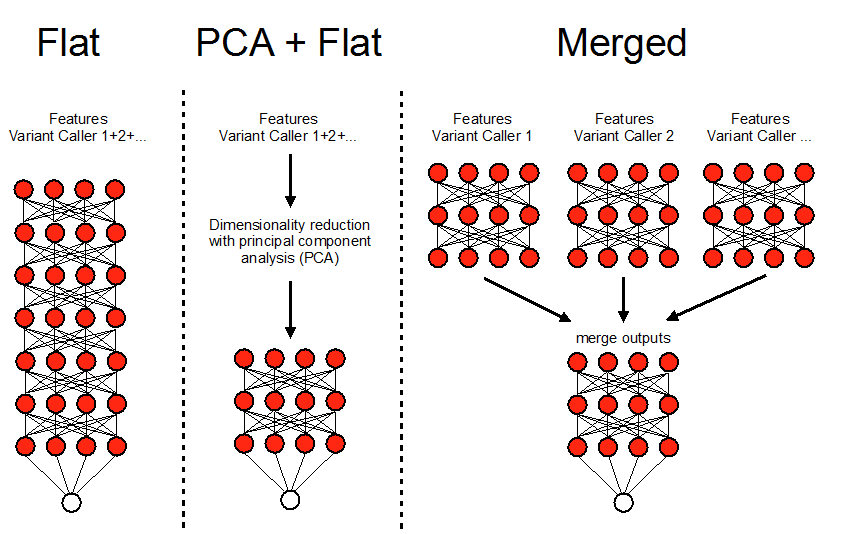
\includegraphics[width=\textwidth]{neuralnetworkstructure.png}
\centering
\caption{\textbf{Different Designs for Neural Network Architecture}}
\end{figure}

We first tested the commonly used flat architecture (Figure 10), which contains stacks of fully connected layers with multiple nodes, initially consisting of seven layers with 80 nodes per layer. In this architecture, all the features from the different variant caller were concatenated into a single vector and used as an input to train the neural network. We found that this architecture was not able to learn from the features, resulting in poor precision (0.0592) and F1 scores (0.111) (Figure 12), suggesting that the number of features might be too high for the flat architecture. 

To address this, we explored the use of principal components analysis as pre-processing step to reduce the number of dimensions prior to the input layer of the flat neural network architecture. Principal components analysis (PCA) is a dimensionality reduction technique that enables a compressed representation of data (Chen et al., 2014; Van Der Maaten, Postma \& Van den Herik, 2009). Each principal component is a linear summation of the original features ($X$) in the form 
\begin{align*}
&PC_1 = \beta_{1,1}*X_{1} + \beta_{2,1} X_{2} +... + \beta_{n,1} X_n \\
&... \\
&... \\
&PC_i = \beta_{1,i}*X_{1} + \beta_{2,i} X_{2} +... + \beta_{n,i} X_n
\end{align*}
which enables a few principal components to capture a high amount of variance in the dataset.

By performing this procedure, we reduced the features to 8 principal components that we used for the inputs to the neural network. However, this reduction in features did not result in appreciable learning in the network, as evidenced by the poor precision (0.0734) and F1 scores (0.136) (Figure 12).

We reasoned that the architecture was not able to learn because of the multimodal nature of the features from each variant caller. To accommodate the multimodal data, we used a merged network architecture consisting of smaller subnets (five layers, 24 nodes per layer) for each variant caller, before merging the outputs in a common network produces the final prediction of a high-confidence variant call (Figure 10). Merged networks have previously been shown to be able to successfully integrate information from multi-modal datasets (Eitel, 2015; Suk, Lee \& Shen, 2014). This architecture proved to be capable of integrating the various complex features, resulting in significantly higher precision (0.877) and F1 scores (0.929). 

\begin{figure}[H]
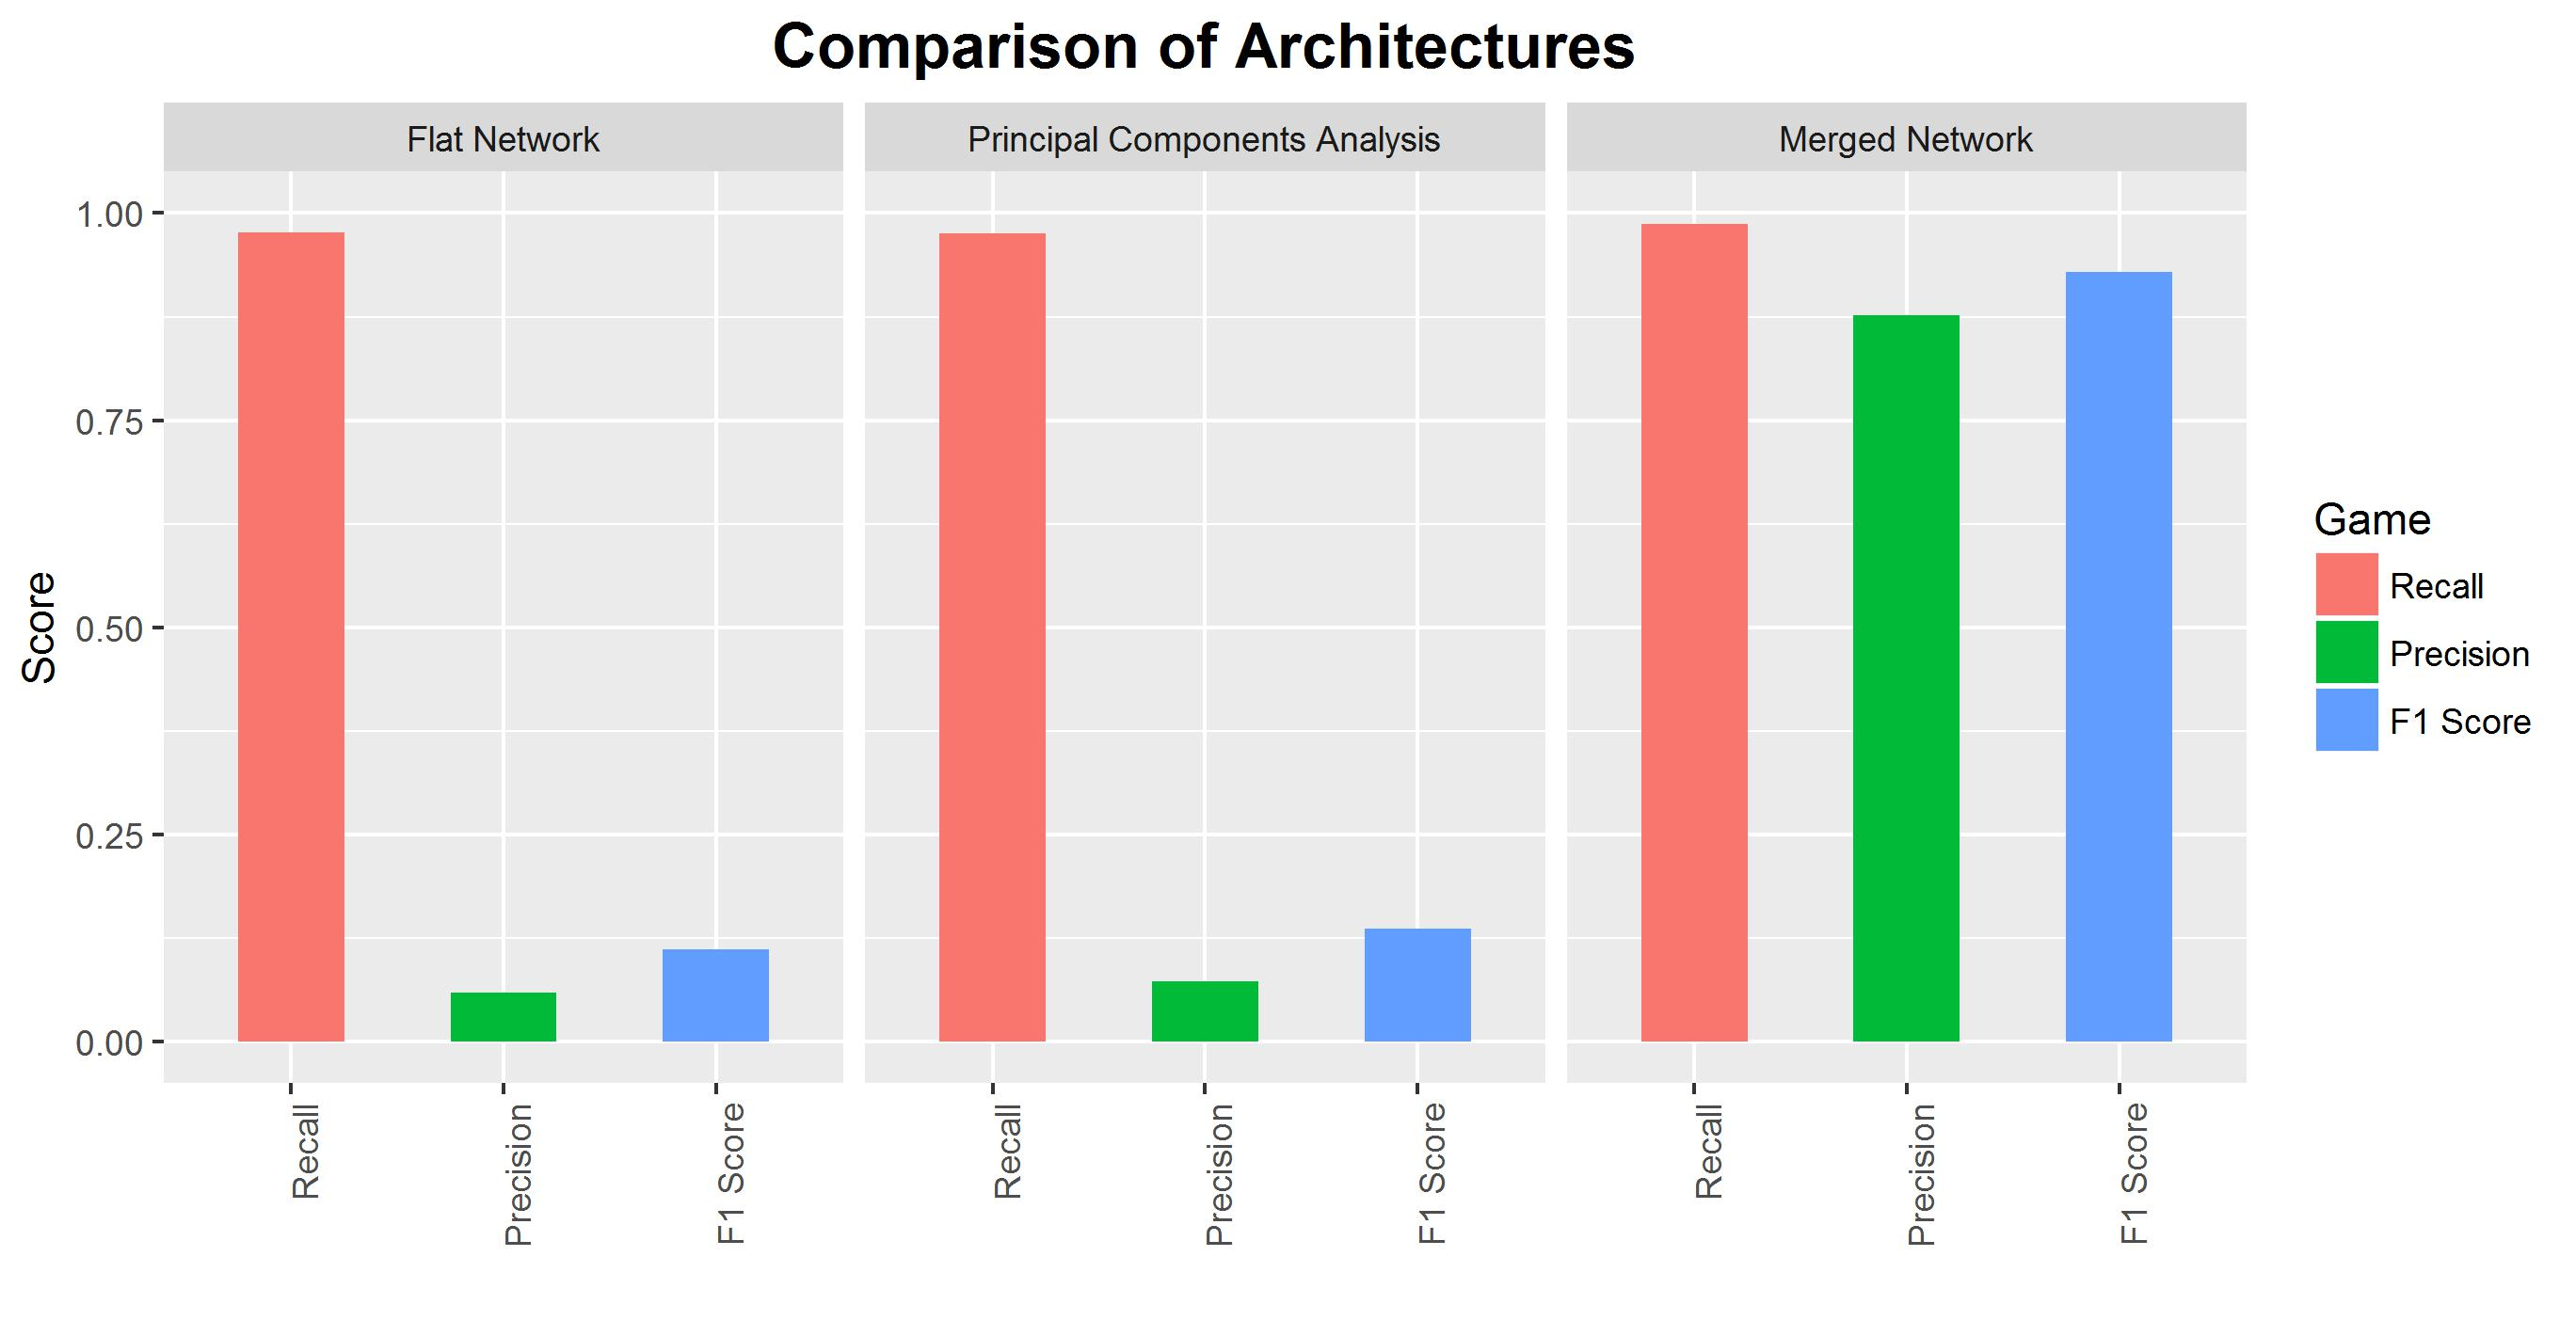
\includegraphics[width=\textwidth]{neuralnetworkstructureresults.jpg}
\centering
\caption{\textbf{Analysis of Different Neural Network Architecture}}
\end{figure}

In summary, we were able to identify a network architecture that could predict high-confidence variant calls from a synthetic dataset by addressing the multimodal nature of the data. The two other networks were not able to learn, resulting in poor precision and F1 scores. Interestingly, the recall scores for all three architectures were around the same ($\pm 0.01$), indicating the main difference for the merged network architecture was in its ability to remove false positive calls.

\subsection{Network Tuning and Optimisation}
Next, we systematically optimised and tuned the deep learning neural network to maximise its predictive ability. To do this we focused on 4 parameters that are known to be critical in deep learning networks (Ruder et al., 2016; LeCun, Bengio \& Hinton, 2015; Yan et al., 2015;  Sutskever et al., 2013), specifically the (i) number of layers; (ii) optimiser choice, (iii) learning rate and (iv) balancing of positive and negative training samples.\\\\
\subsubsection{Number of Layers}
Firstly, we evaluated how the number of layers affects the performance of the neural network, as the number of layers determines the representation of data that can be captured by the neural network. The number of layers can affect the network in two ways -- increasing the number of layers can enable complex data representation needed for learning, but excessive layers might result in the vanishing gradient problem (Sutskever et al., 2013; Bengio et al., 1994), where the signals are unable to propagate across too many layers.

Using our merged network architecture as a foundation (Figure 13), we varied the number of layers in the pre-merge networks that were specific for each caller and the common network after the merge layer.
\begin{figure}[H]
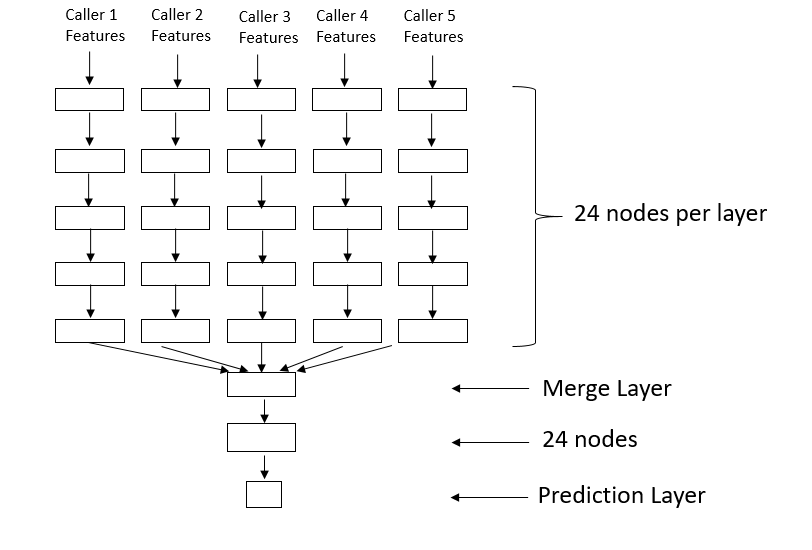
\includegraphics[width=\textwidth]{neuralnetworkarchitecturefinal.png}
\centering
\caption{\textbf{Basic Merge Network Structure.} Each individual pre-merge layer takes in an input feature vector from a single caller. The information is then integrated in a set of merge layers to give a prediction.}
\end{figure}
 We observed that changing the number of layers after the merge layer did not significantly vary the performance. Thus we focused on changing the number of layers before the merge layer. We compared six different neural network structures ( four layers to nine layers) using accuracy was used as the main metric, which is defined as the fraction of all samples that the neural network can correctly predict.
\begin{figure}[H]
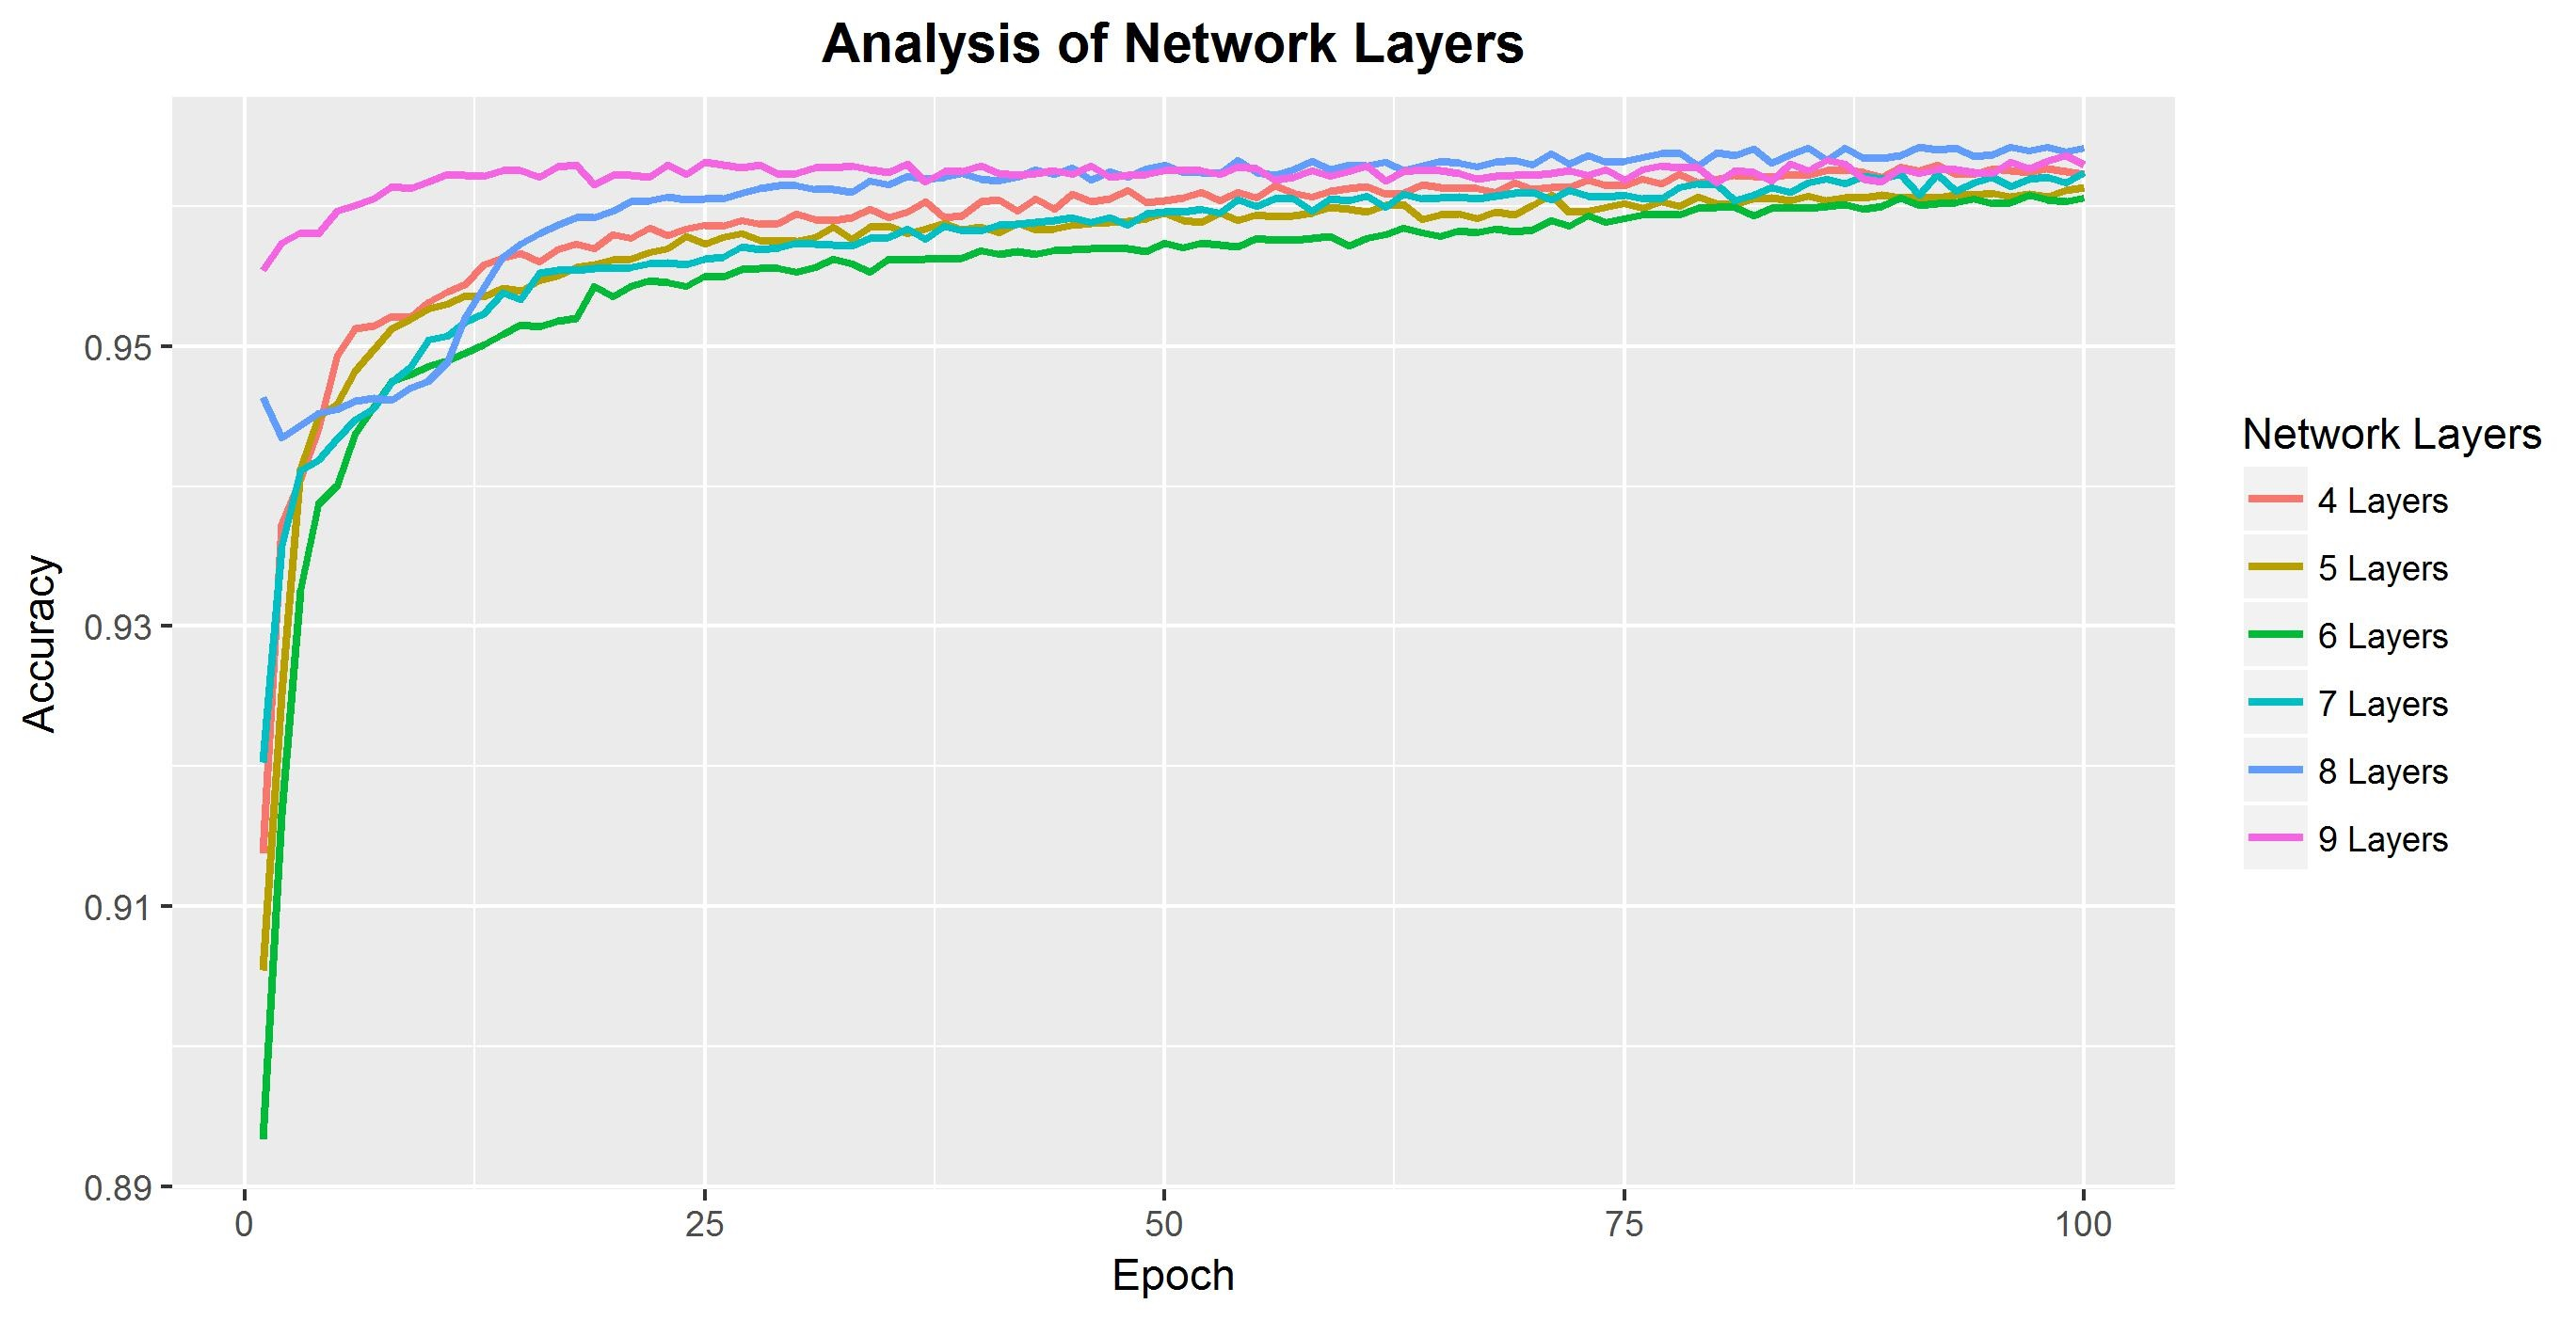
\includegraphics[width=\textwidth]{networkstructuredataset.jpg}
\centering
\caption{\textbf{Analysis of Different Number of Layers On Training Accuracy}}
\end{figure}
We found that all the different layered network were able to learn, but the eight layer neural network performed the best at learning from the input data, with a final accuracy of 0.964 approximately 0.001 higher than other layers.     
\subsubsection{Optimiser and Learning Rates}
Next, we sought to choose the best optimiser and learning rate for our eight-layer network. Both optimisers and learning rates have been shown to be important in neural network training (Ruder et al., 2016; Sutskever et al., 2013).\\\\
Optimiser choice is critical as the optimisers determine how the weights and gradients are updated in the network, thus playing an integral part in learning. We evaluated three standard optimisers for use in our network, ADAM, RMSprop and Stochastic Gradient Descent (SGD). ADAM is an adaptive learning rate optimiser that is known to be well suited in large dataset and parameter problems (Kingma \& Ba, 2014). RMSprop is another adaptive learning rate optimiser that has been shown to work well for real experimental datasets (Tieleman \& Hinton, 2012). SGD is the simplest learning model with no adaptive learning rate but is a useful model because it is the easiest to understand mathematically and has also been shown to solve deep learning problems (Kingma \& Ba, 2014).  Further information on the mathematical foundations of optimisation and backpropagation, can be found in Appendix 5.1. 
\begin{figure}[H]
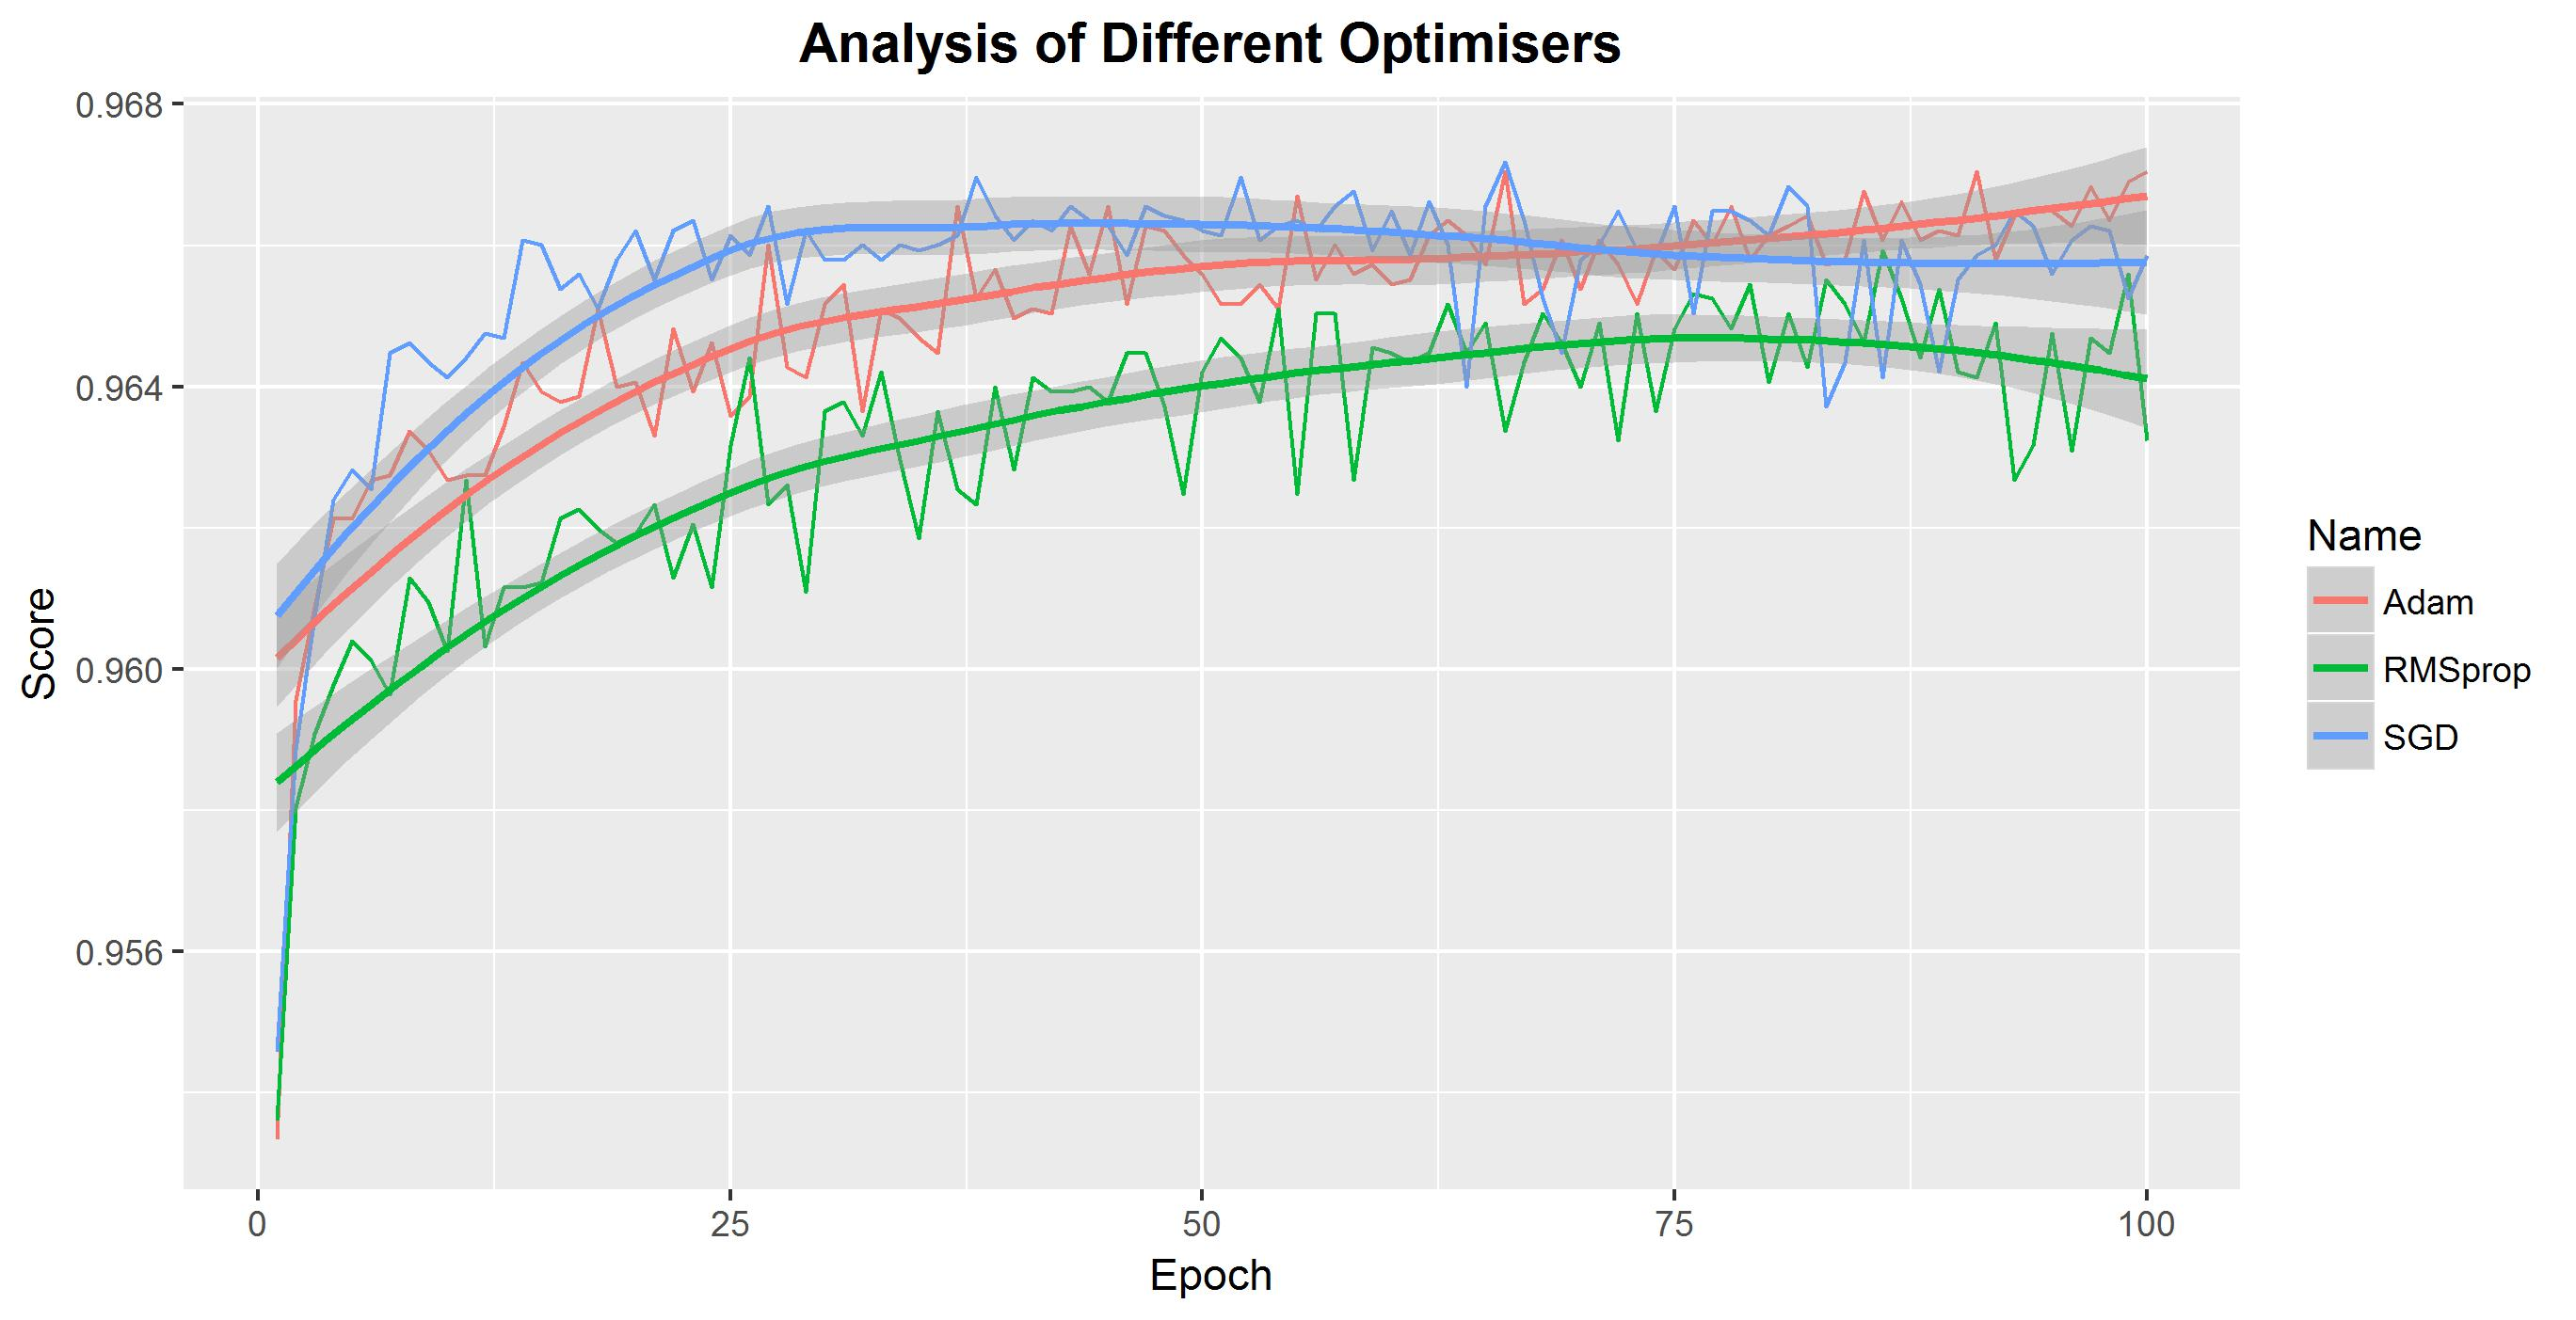
\includegraphics[width=\textwidth]{optimiserlearning.jpg}
\centering
\caption{\textbf{Optimiser Accuracies for Training at each Epoch.} Due to the accuracy noise, the overall momentum of the dataset, calculated as a sliding window average is shown. The 95\% confidence interval is also shown.}
\end{figure}

We evaluated the accuracy of the neural network running on each of the three optimisers (Figure 14). We found that Adam obtained the highest accuracy of 0.9670, while RMSprop and SGD reached maximum accuracies of 0.9660 and 0.9569 respectively. Interestingly, the adaptive rate optimisers seemed to have complex learning trajectories, while SGD has a very stable learning rate. This is consistent with that fact that adaptive learning rates allow greater gradient descents when the error is high while decreasing the learning rate when the error is low (Kingma and Ba, 2014; Zeiler, 2012). This adaptive capacity enables Adam and RMSprop to learn at variable rates based on the current gradients. In contrast, SGD requires more time to learn the true minima, but eventually still reaches about the same minima as RMSprop.\\\\
We chose Adam as our optimiser as (i) the final accuracy discovered by Adam was noted to be higher than RMSprop and SGD, and (ii) the  learning curve for Adam was stable, indicating it is able to learn and update the gradients in the neural network to learn from input data at all epochs.\\\\
Finally, we evaluated initial learning rates for the Adam optimizer (Figure 16). We found that the most stable learning trajectory was observed at a learning rate of $10^{-5}$. This initial learning rate is critical as it determines the first few gradient descents which enable stable adaptive learning throughout the epochs (Sutskever et al., 2013). At higher learning rates ($10^{-4}$ and below), a very high amount of noise was observed, indicating that the learning rate was too high resulting in a difficulty in finding the minima. At lower learning rates ($10^{-6}$ and above), the final accuracy after 100 epochs (0.9639 for $10^{-6}$) was lower than the learning rate at $10^{-5}$ (0.9672). Thus, we concluded that $10^{-5}$ was the optimal learning rate for our network.
\begin{figure}[H]
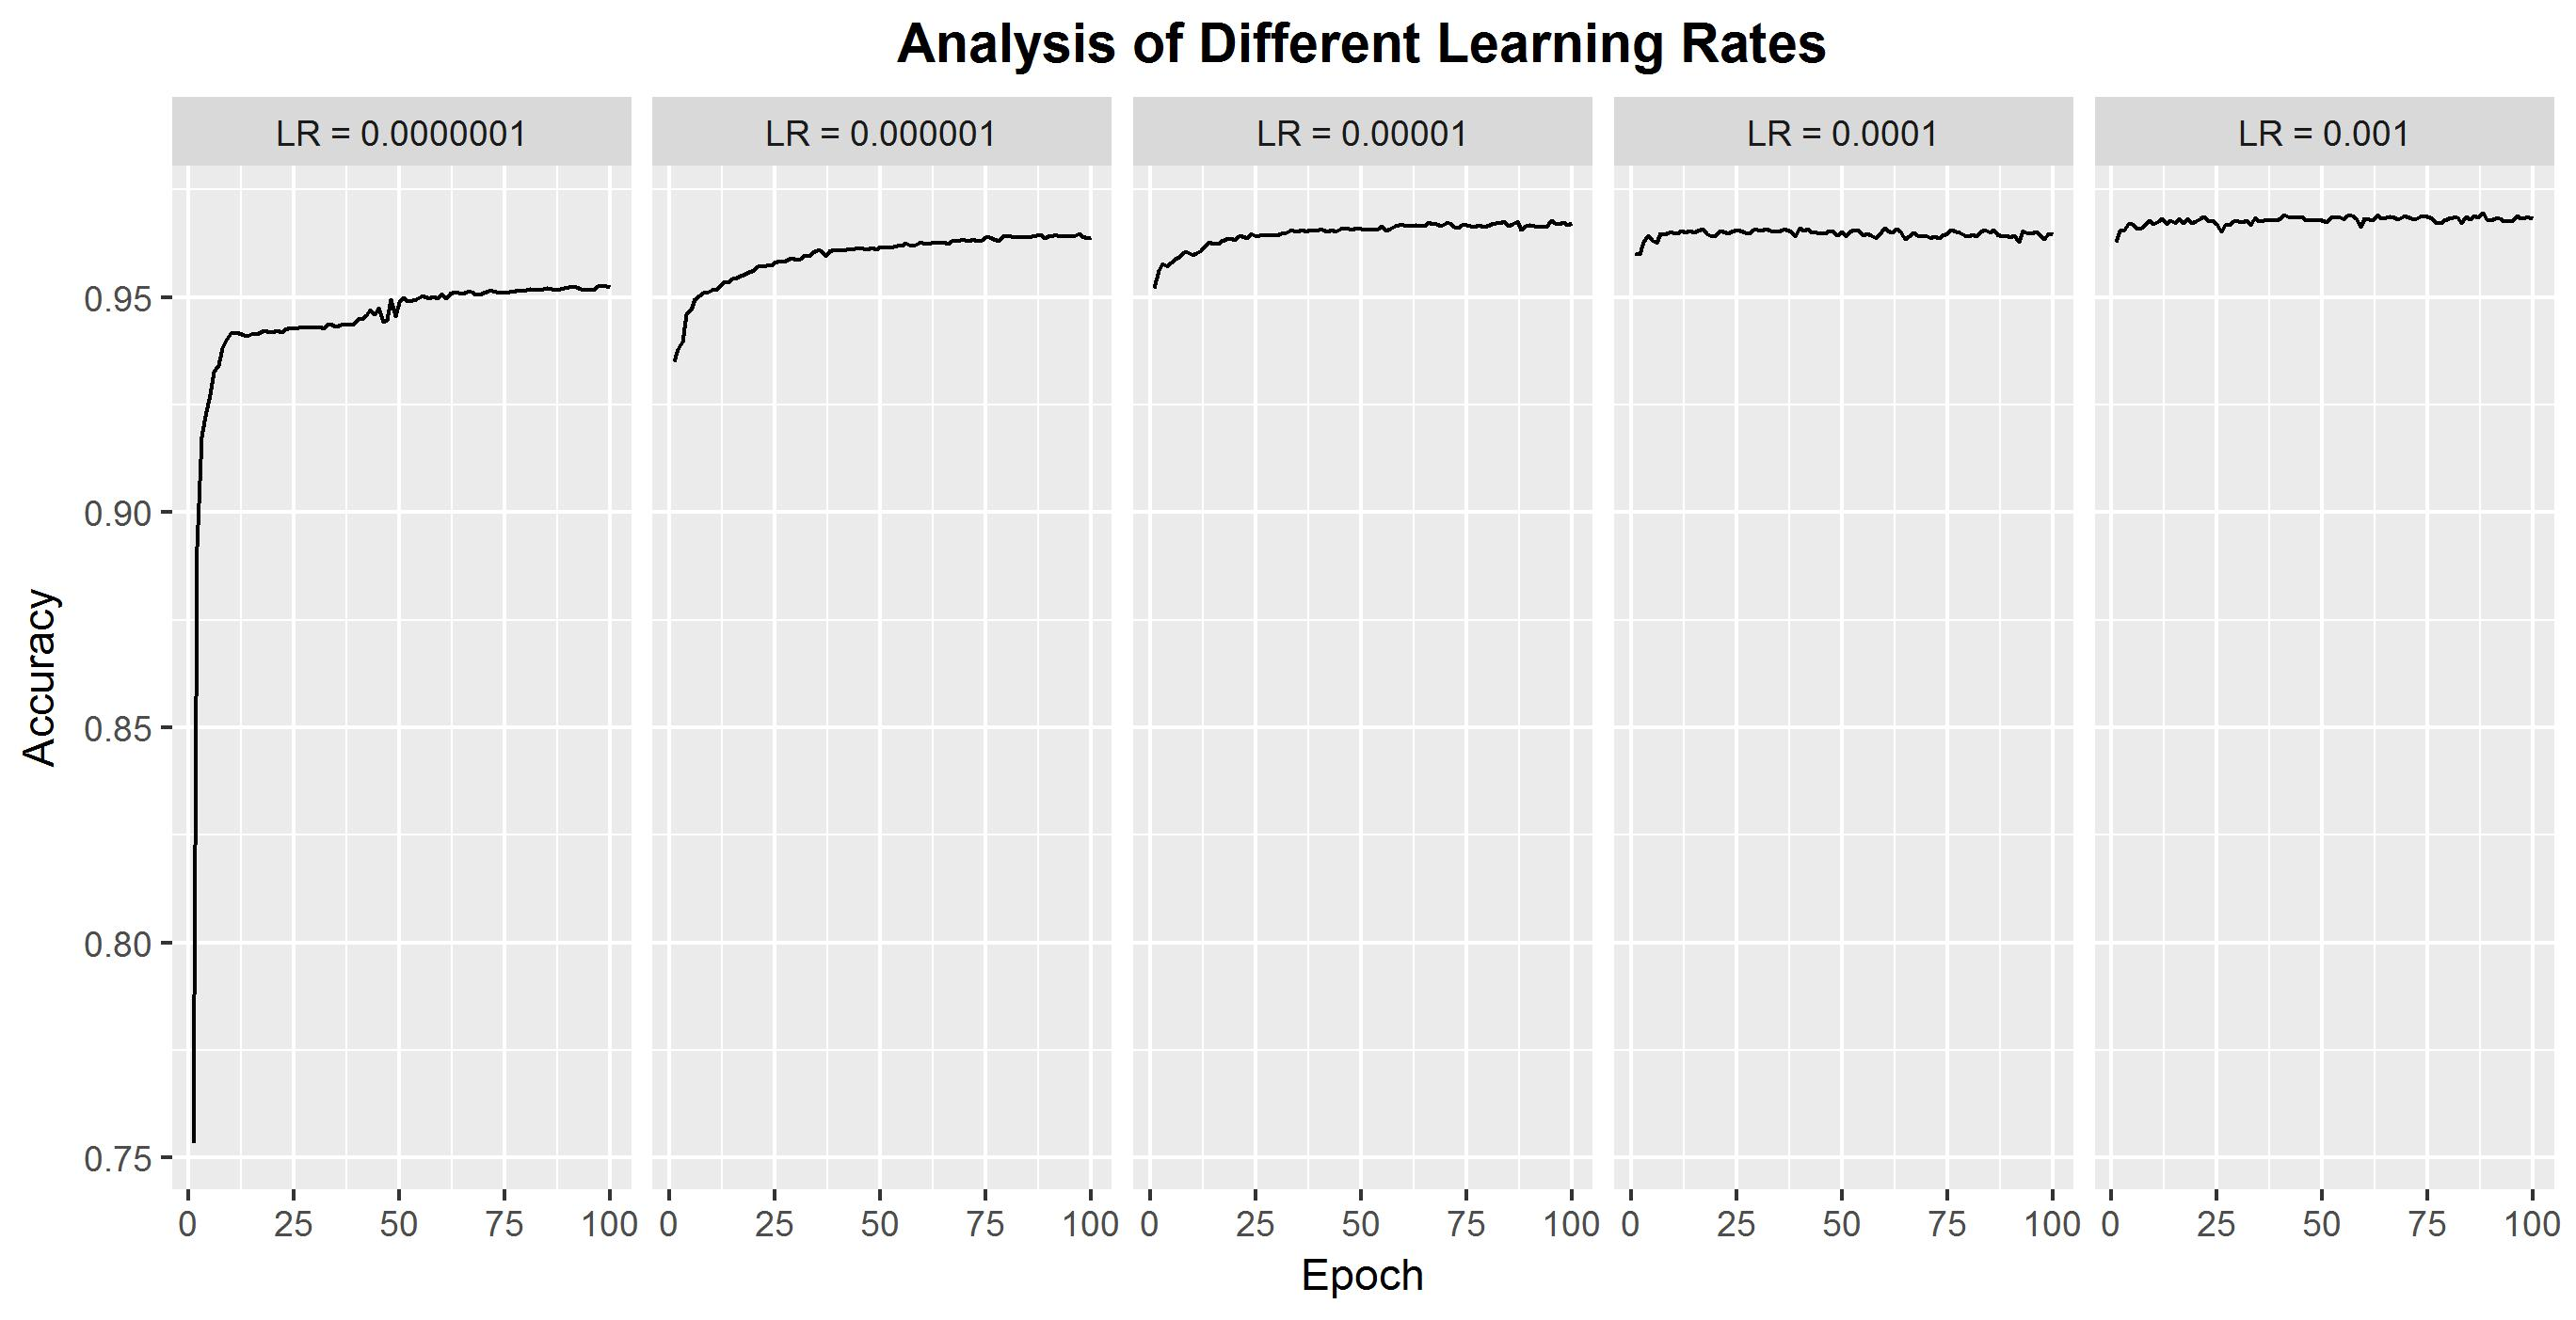
\includegraphics[width=\textwidth]{learningrates.jpg}
\centering
\caption{\textbf{Training Accuracies over Each Epoch for Different Learning Rates}}
\end{figure}
\subsubsection{Sample Balancing}
We considered whether the imbalance in samples would affect the performance of the network, given the synthetic dataset contained an abundance of positive training examples compared to negative training examples. In total, there were 286,510 positive training examples and 4,547,919 negative training examples (about a 15-fold difference). Sample imbalances in the training data have been known to affect learning adversely (Yan et al., 2015; López et al., 2012). Thus, we wanted to determine if correction of imbalances would improve network performance by using two different methods of sample balancing: undersampling and oversampling. In the undersampling approach, negative training examples were removed until the number of negative training examples was equal to the number of positive training examples. In oversampling approach, we used that Synthetic Minority Oversampling Technique(SMOTE) algorithm, which uses nearest neighbours to impute additional data points for the positive training example. In other words, SMOTE examines two nearby positive class examples and creates a new synthetic example in the middle of these two examples (see Appendix 5.3.3 for more details).
\begin{figure}[H]
\centering
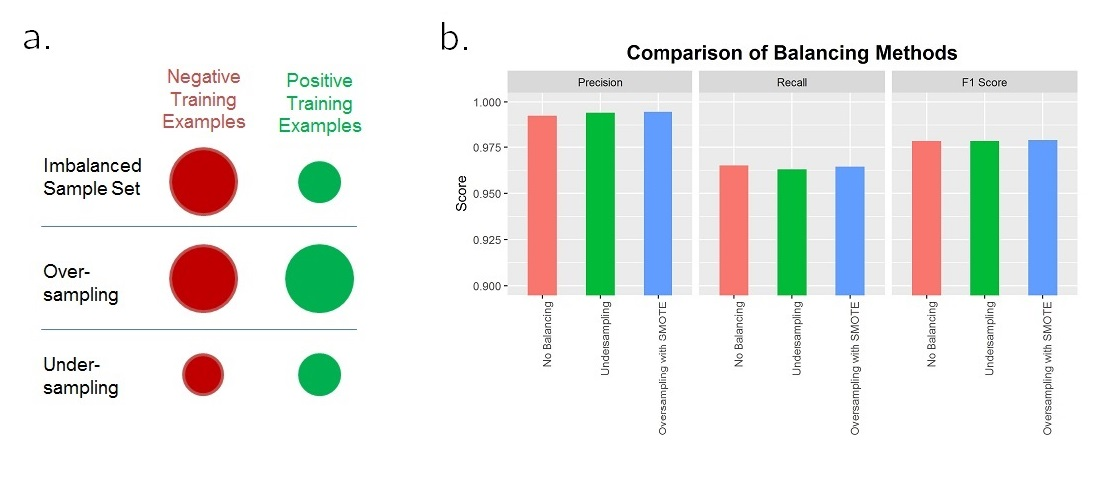
\includegraphics[width=\textwidth]{comparisonofbalancingmethods.jpg}
\caption{\textbf{a)} \textbf{Graphical Illustration of Sample Balancing.} \textbf{b) Effect of Sample Balancing Techniques on Prediction Ability.}}
\end{figure}
Interestingly, we note that overall, undersampling, oversampling and no sampling at all had very small effects on precision, recall and the final F1 score (Figure 17). Specifically, all three metrics were within a range of 0.003 for the different sampling techniques. We suspect that sample balancing did not significantly improve the performance because the synthetic dataset may have clearly separable positive and negative examples that would not benefit from any sampling.\\\\
However, we noted that oversampling techniques resulted in a marginally higher F1 score (0.001 higher than undersampling and no sampling), and because balanced datasets can minimise further bias in downstream analyses (Chawla, 2005), we used SMOTE oversampling to balance the training samples for all the network analysis.
\subsection{Benchmarking of Optimised Network with Mason Dataset}
Following optimisation steps, we finalised the network architecture as similar to that in Figure 9, but with eight layers before the merge layer. We chose the Adam optimizer with a learning rate of $10^{-5}$. With this network configuration, we benchmarked the neural network against the single variant callers, as well as concordance callers, which are an integration of the outputs of the five variant callers. Specifically, the n-concordance variant caller is defined as the set of calls that any n callers agree upon -- so 1-concordance includes all the calls made by all callers and 4-concordance includes all the calls made by any 4 callers.
\begin{figure}[H]
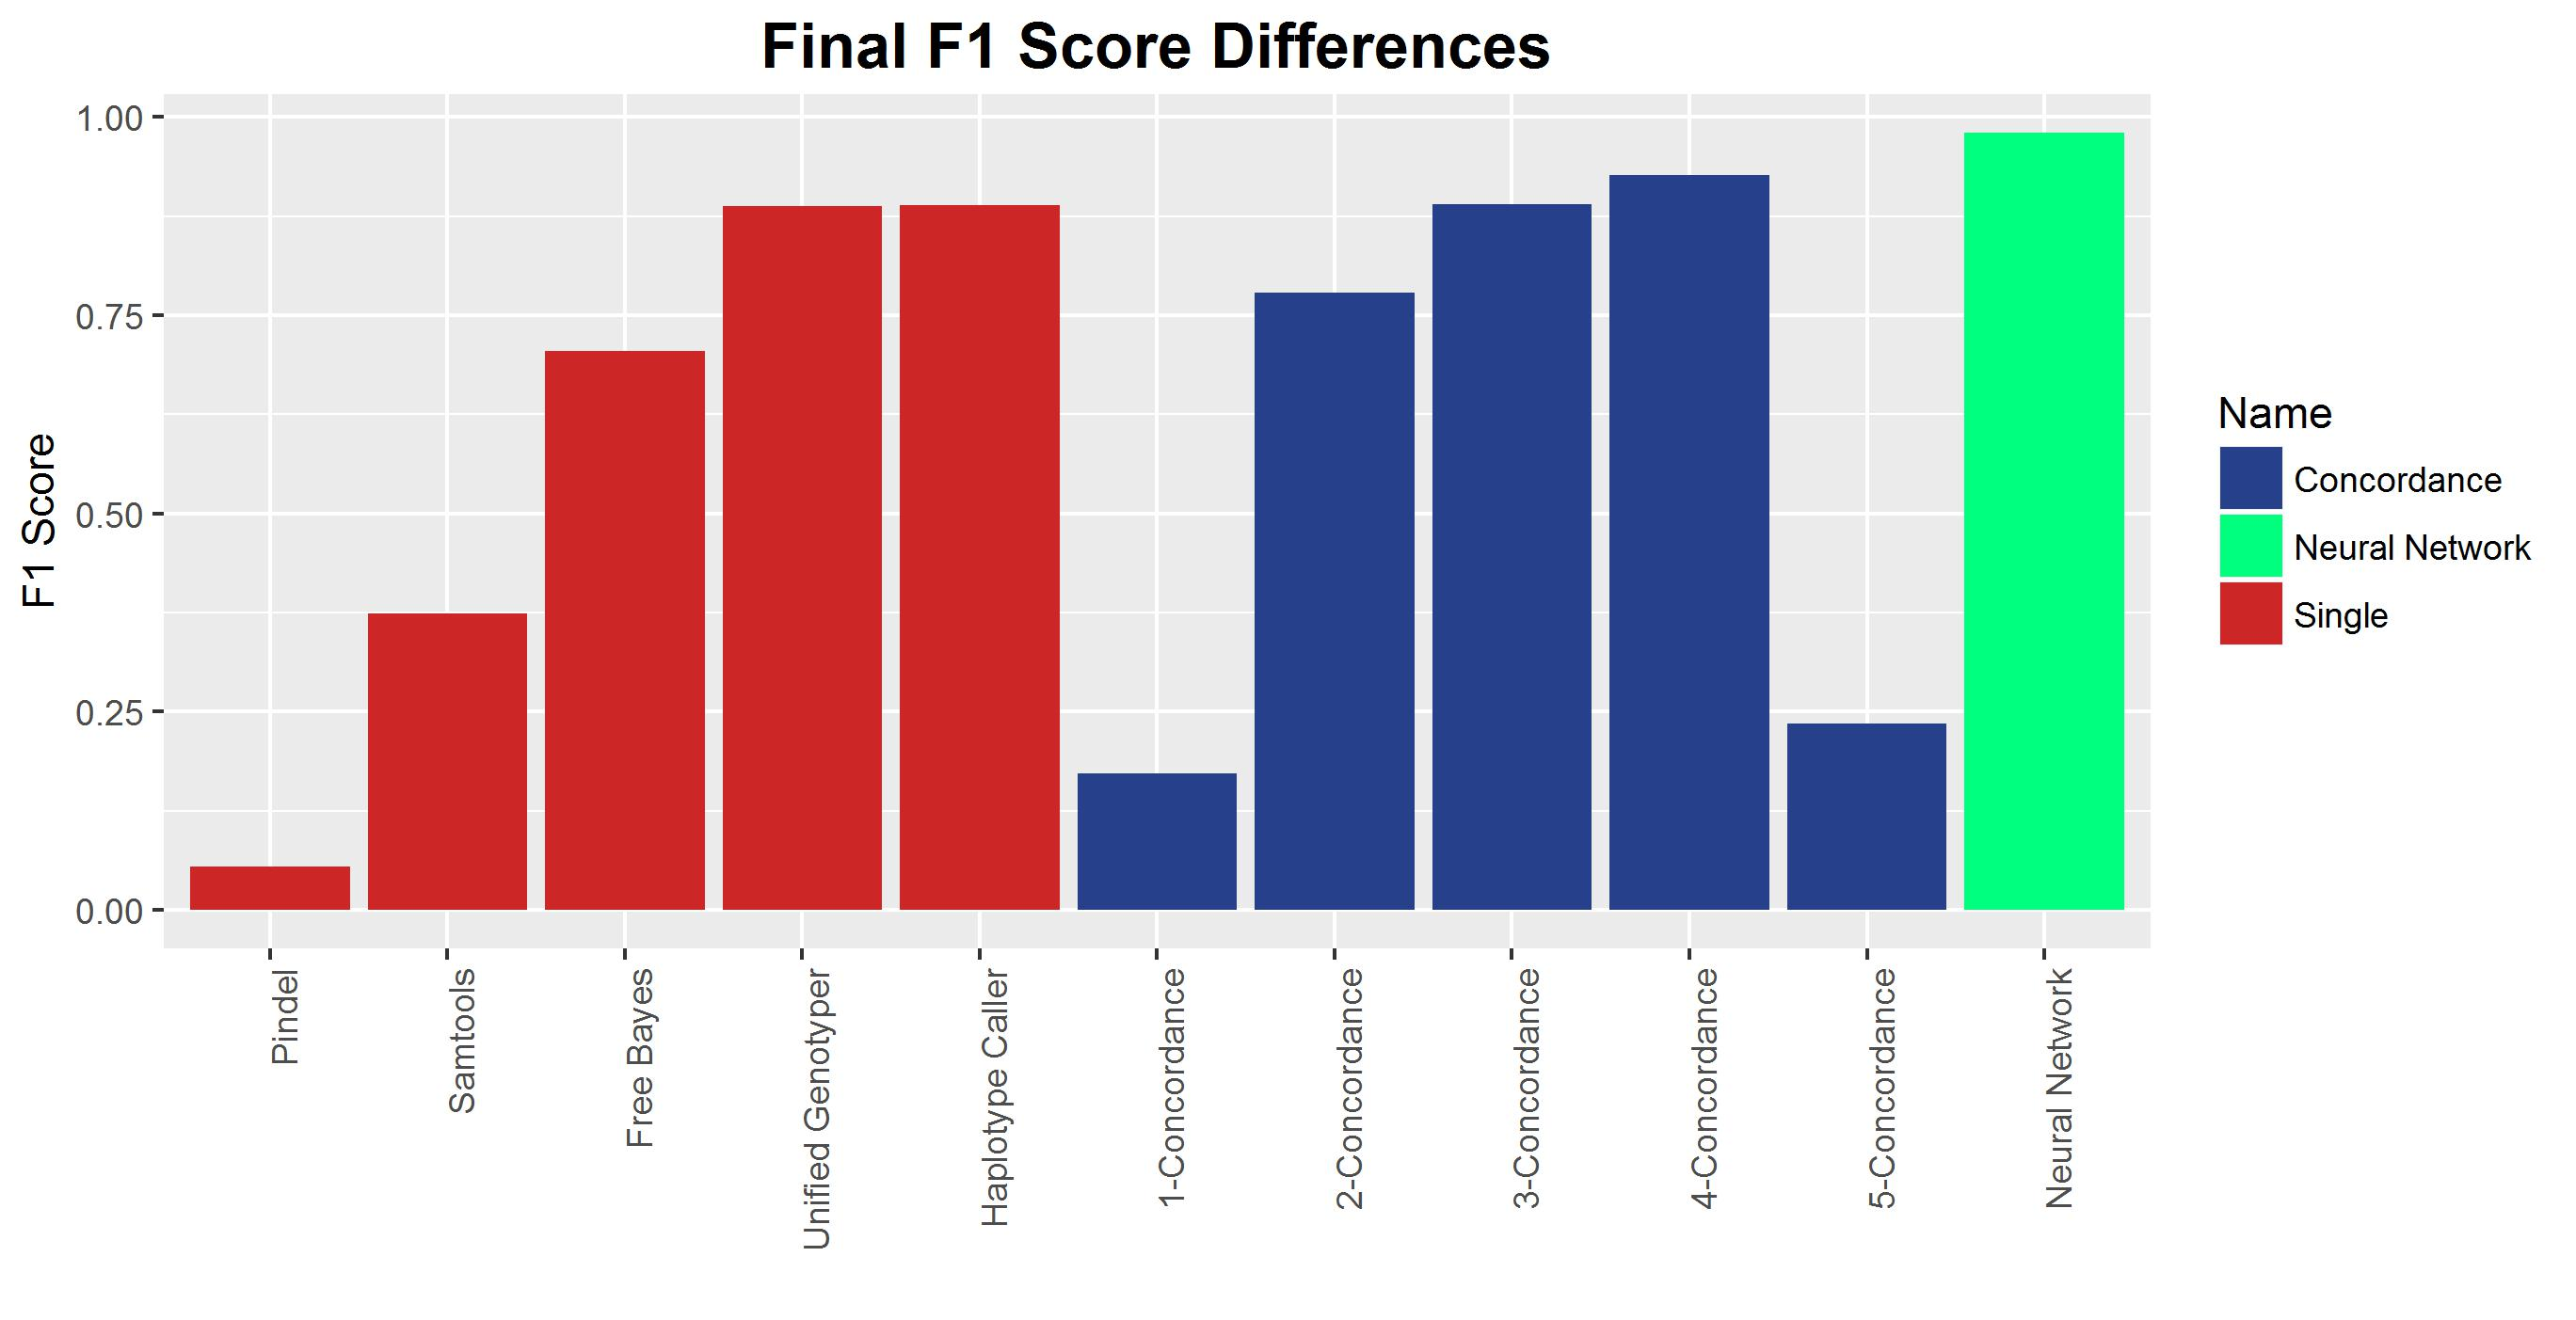
\includegraphics[width=\textwidth]{final_f1scores_results_all.jpg}
\caption{\textbf{Overall Comparison of Variant Callers}}
\centering
\end{figure}
Using the overall F1 score as the performance metric (Figure 18), we found that the neural network was able to outperform single and concordance-based callers. This provides strong evidence that the neural network can learn from the input features to identify high-confidence variant calls. The final F1 score obtained by the best single variant caller was the GATK Haplotype Caller at 0.888, and the best concordance caller had an F1 score of 0.927, while the neural network achieved the highest F1 score of 0.980. To gain insight into the improved accuracy, we examined the improvements in the precision and recall scores. We found that the gain in the F1 score is due to the increased precision of the neural network, while the recall scores for different calling strategies was similar (Figure 19). 

\begin{figure}[H]
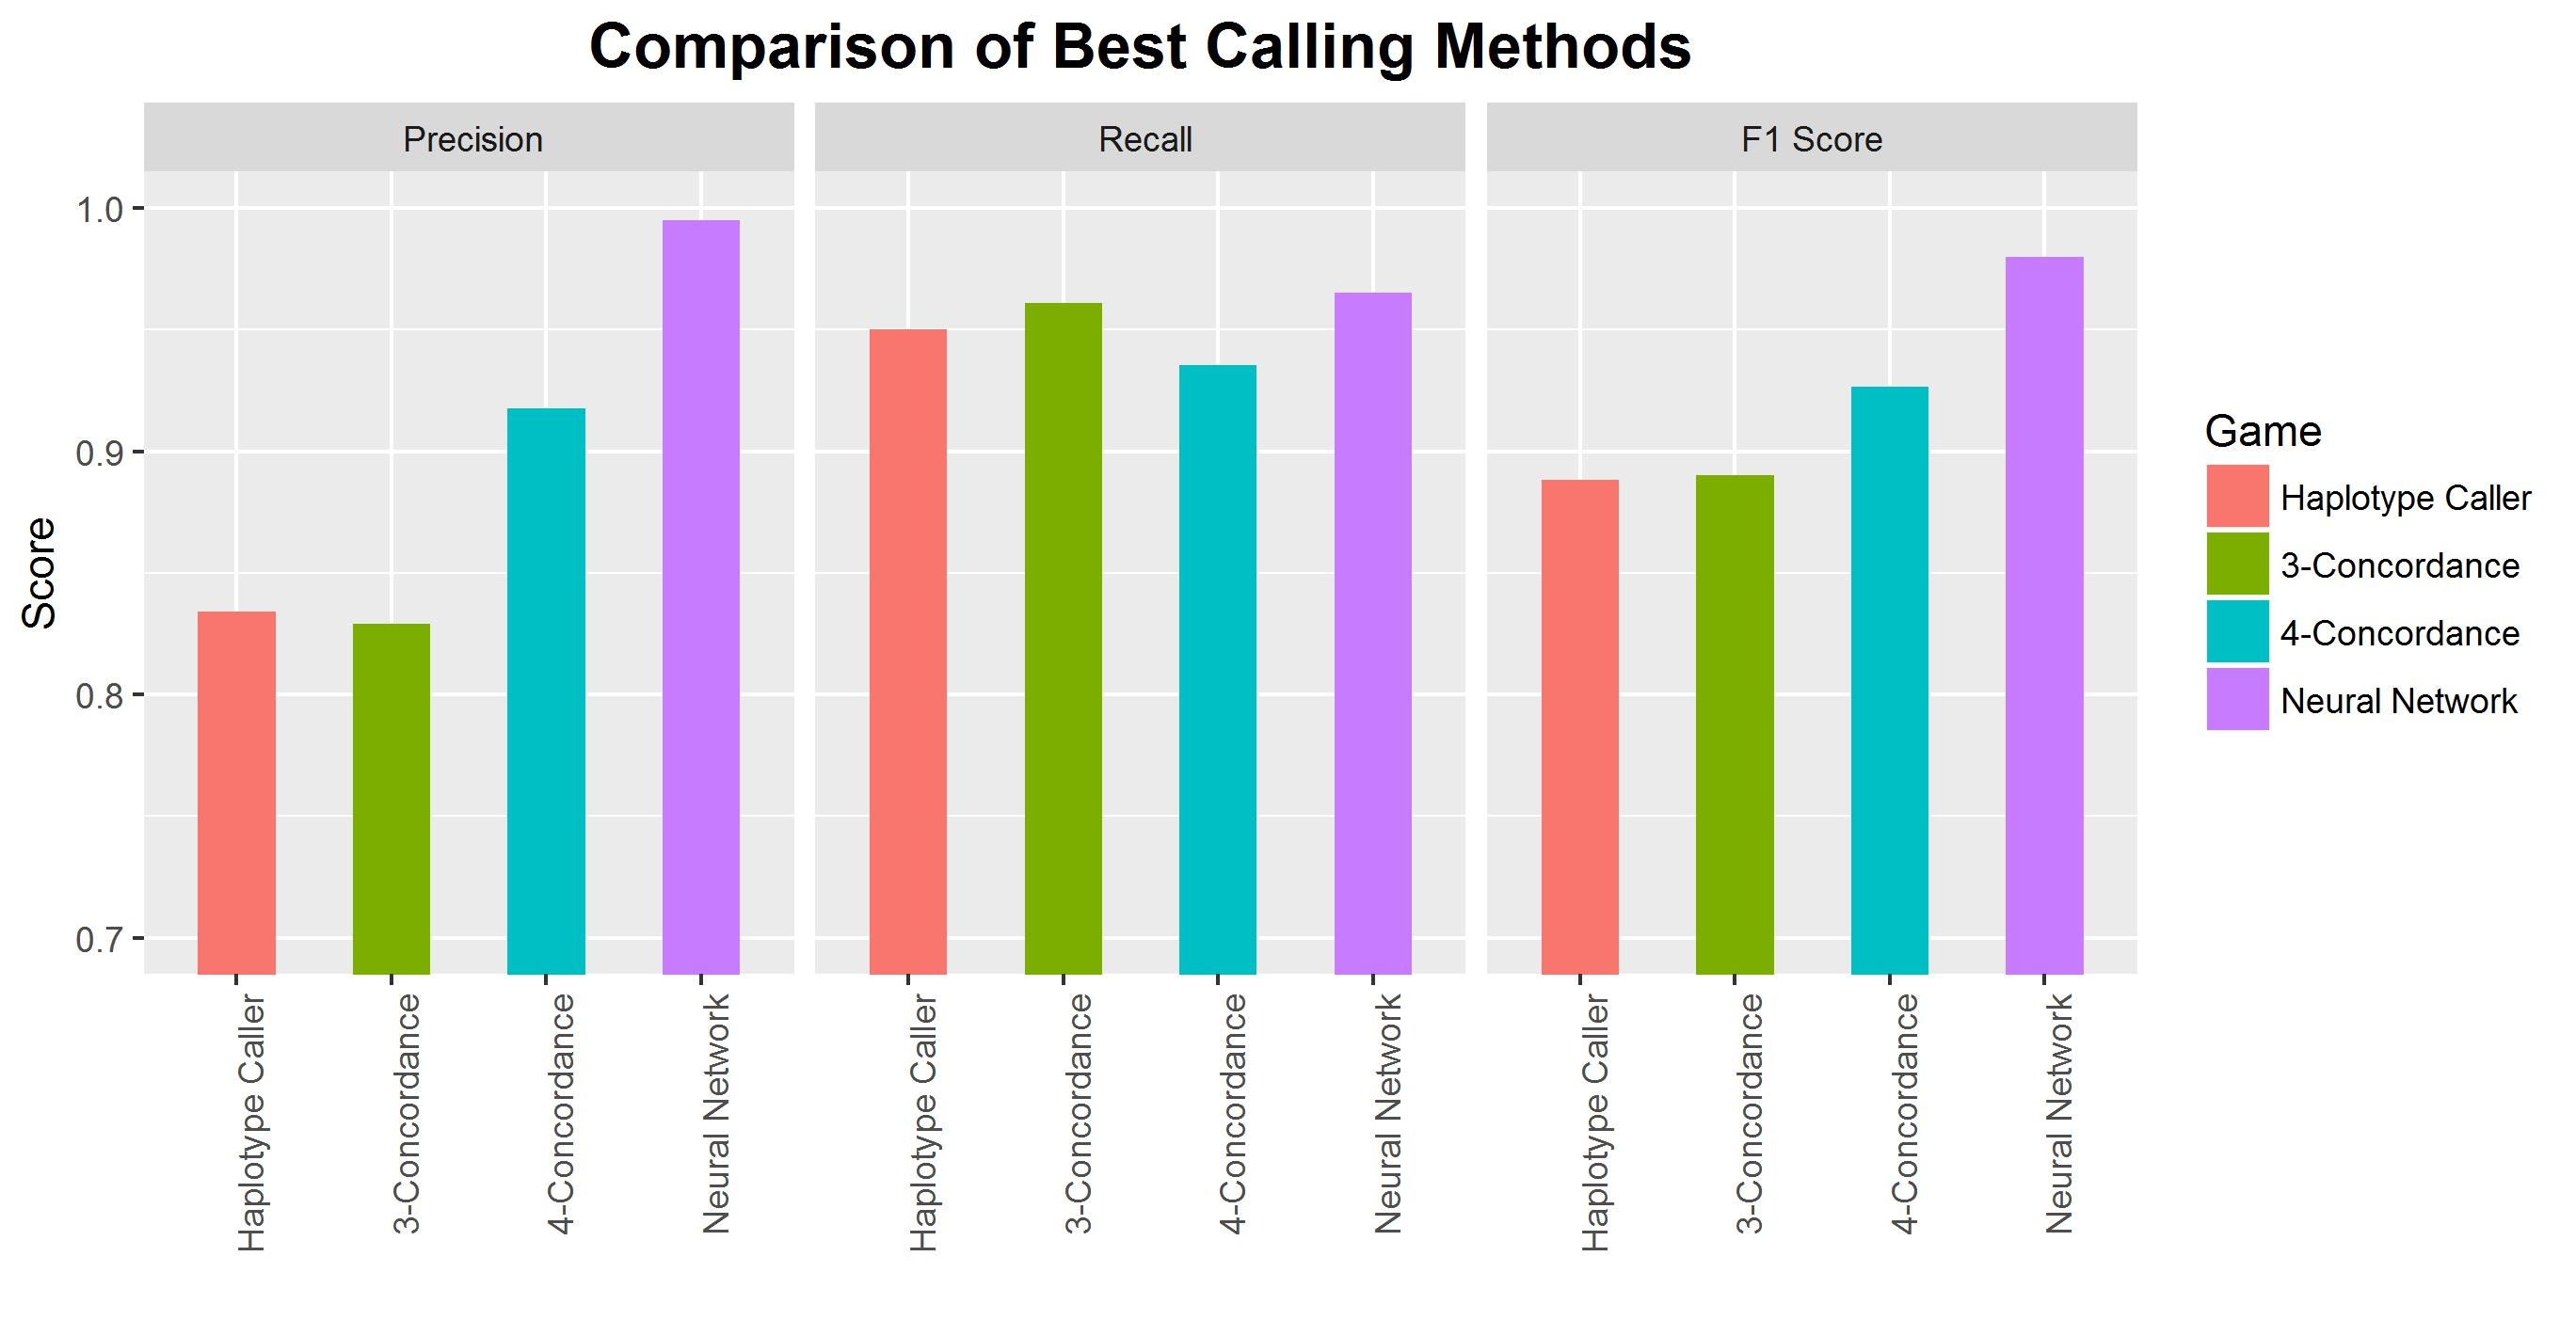
\includegraphics[width=\textwidth]{masonheadsupcomparison.jpg}
\caption{\textbf{Comparison of Best Variant Callers in terms of Precision, Recall and F1 Score}}
\centering
\end{figure}
Closer examination of the performance metrics revealed the neural network had the highest precision of 0.995 compared to only 0.917 for 4-concordance call. This represents a 20 fold decrease in the number of false positives or about 23,000 less false positive calls in the neural network compared to the 4 concordance network. Interestingly, the recall of all the callers was high in the range of 0.90 to 0.95, indicating that while all were able to pick out most of the truth variant calls, the majority of the errors came from a high number of false positives.\\\\ 
In summary, the neural network had an F1 score that was 11\% above the best single caller and 6\% above the best concordance caller. Thus, this provides strong evidence that the neural network can sieve out false positives within the dataset and stably predict whether a mutation is true.
\subsection{Benchmarking of Optimised Network with NA Dataset}
After validation of the optimised neural network on the synthetic dataset, we next tested the performance of the neural network on a real dataset. To do this, we used the NA12878 Genome In a Bottle dataset (Zook et al., 2014), which is a reference genome that has been used in other variant calling validation pipelines (Talwalkar et al., 2014; Linderman et al., 2014). This is a real genomic dataset that contains a set of high-confidence variant calls obtained from multiple iterations of sequencing with orthogonal platforms. These platforms include SOLiD, Illumina, Roche 454 and Ion Torrent sequencing technologies. Integrating the calls from multiple sequencing platforms minimises sequencing errors and generates a set of high-confidence calls that can be used for validation pipelines. \\\\ Subsequently, we used the NA12878 dataset and accompanying high-confidence variant calls to benchmark the performance of our neural network against the two best concordance callers and the best single variant caller, GATK's Haplotype Caller. 
\begin{figure}[H]
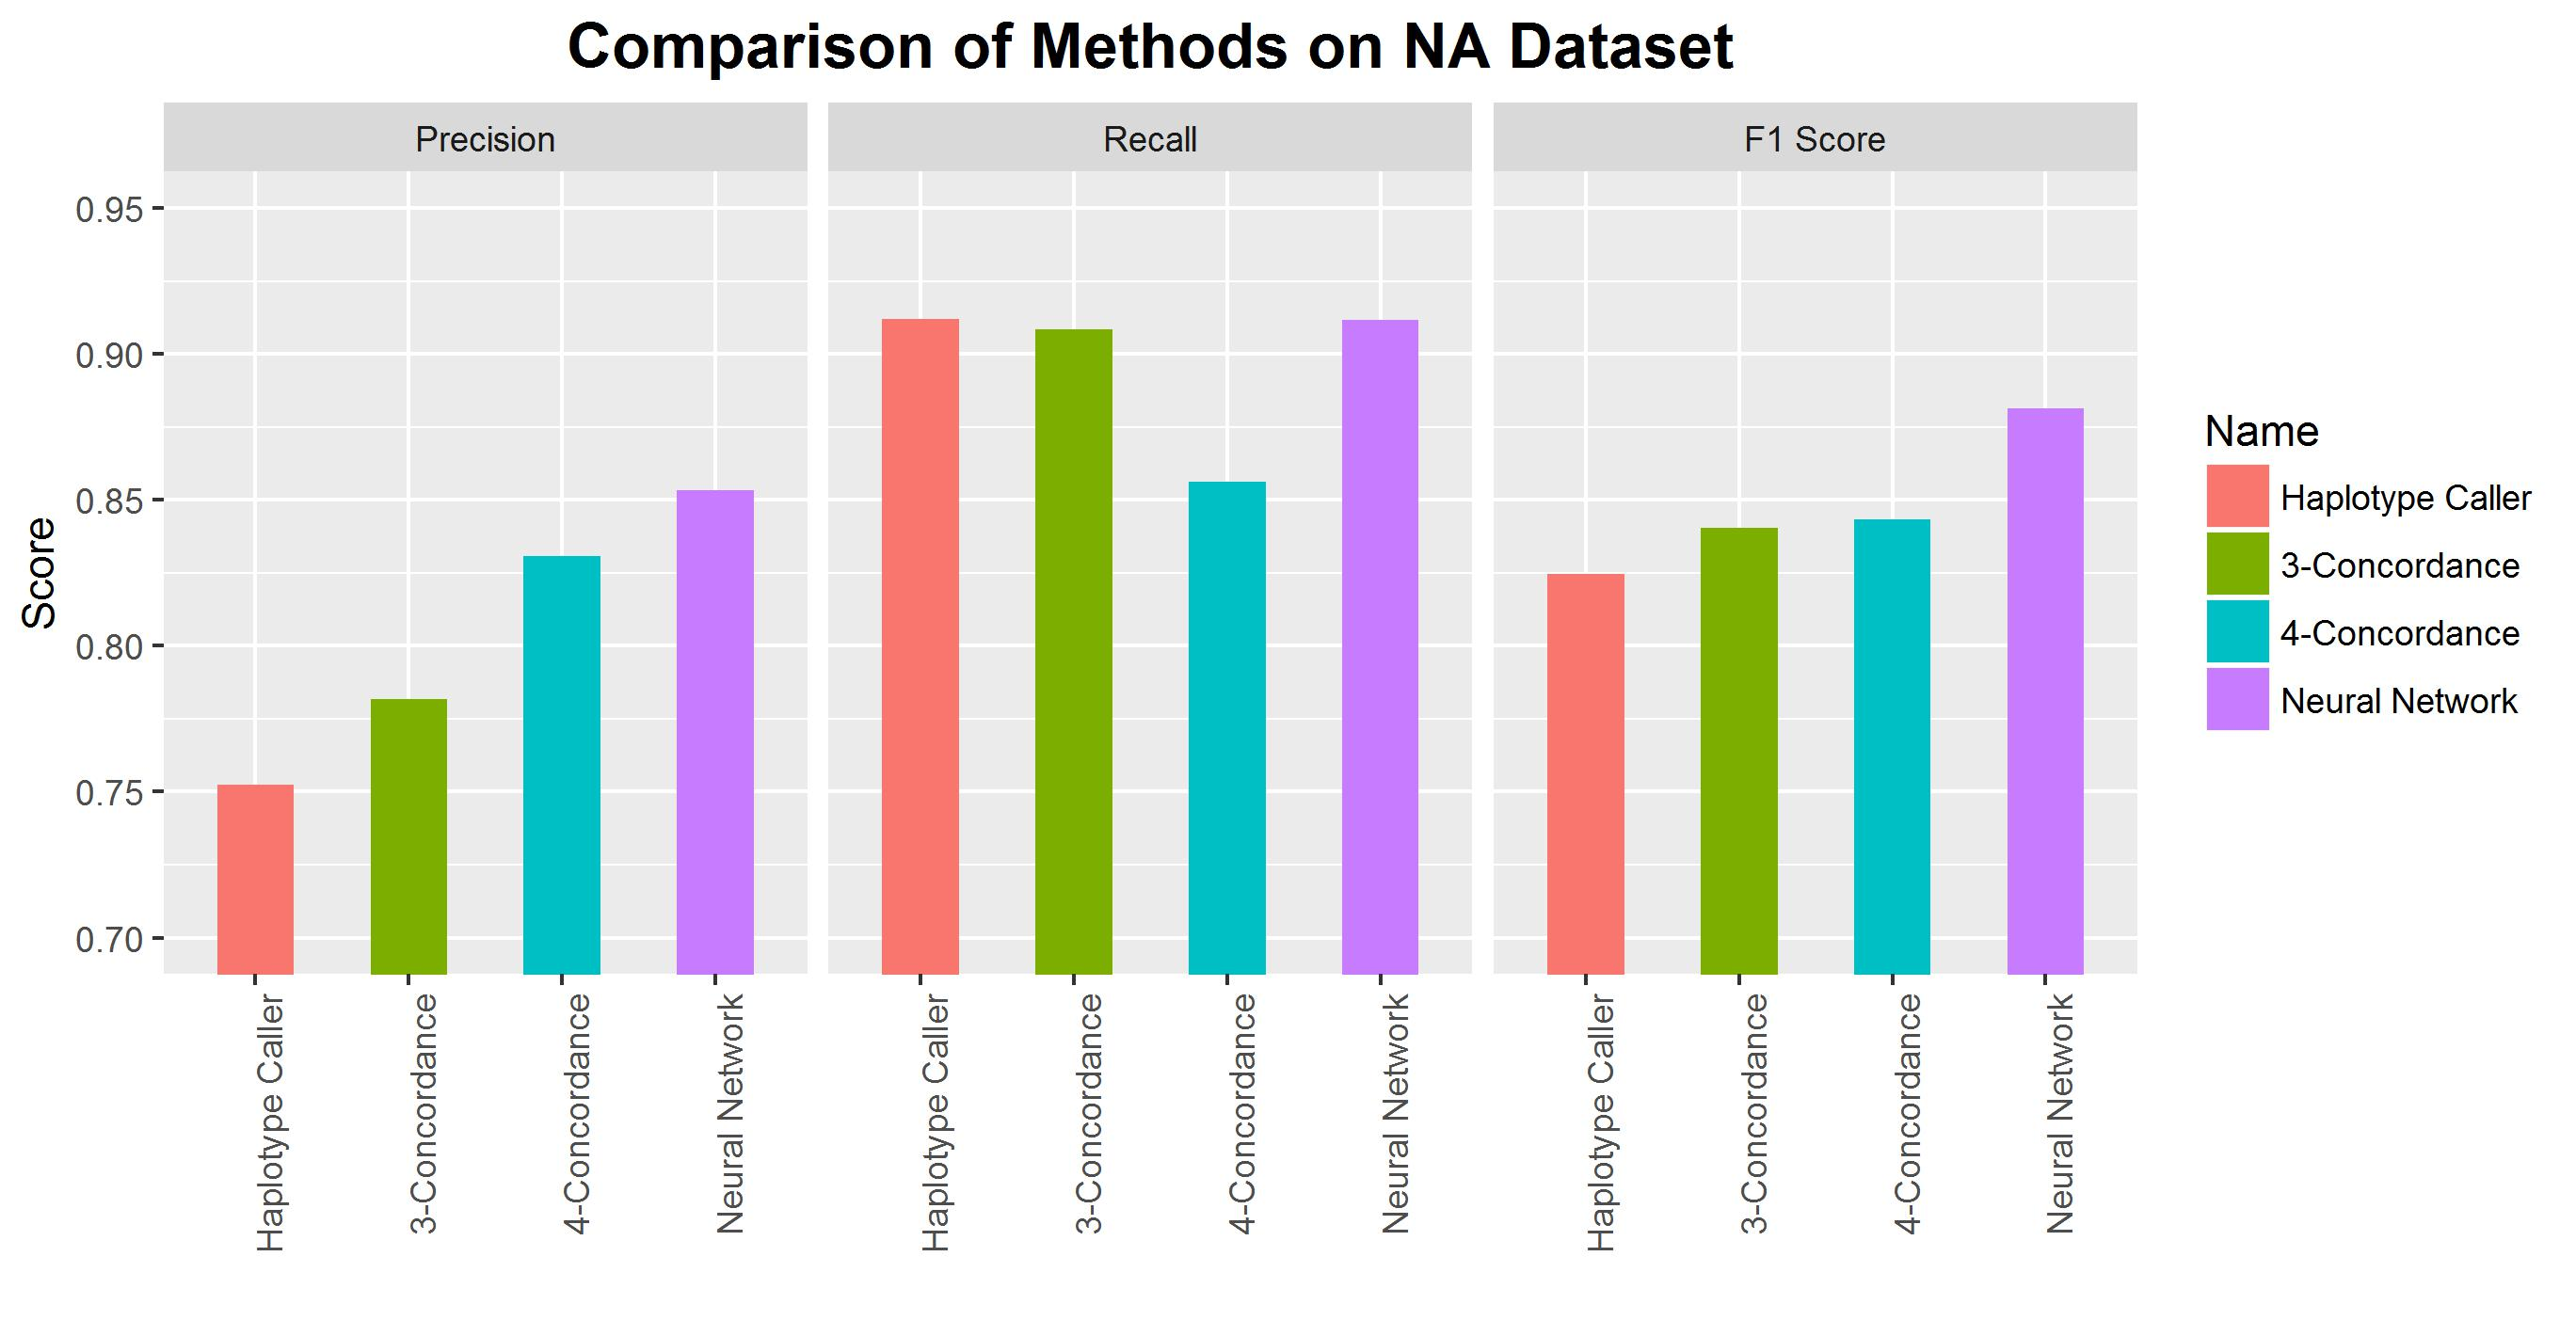
\includegraphics[width=\textwidth]{naheadsupcomparison.jpg}
\caption{\textbf{Comparison of Variant Callers}}
\centering
\end{figure}
In benchmarking with the NA12878 dataset, the neural network had the highest F1 score of (0.882), followed by 4-concordance (0.843) callers, 3-concordance (0.840) and GATK Haplotype Caller (0.825). This indicates that the neural network is also able to predict high-confidence variants in a real dataset. Interestingly, we note that the neural network was more precise and had a higher recall than the 4-concordance caller - it was able to call 2650 more true variants and still had 1228 less false positives. This suggests that the neural network can successfully predict high-confidence calls from discordant calls, thus providing evidence that deep learning is a better technique to integrate variant call information than concordance. 
\\\\
In summary, the neural network was able to outperform concordance variant callers by at least 4.5\% and single callers by 6\% in terms of F1 score. This validates our neural network approach in a real genomic dataset and indicates that network is to stably predict high-confidence variants from the input features.
\newpage
\subsection{Analysis of Variant Importance using Bayesian Ranking systems}
After validation of high confidence calls using a deep learning network, we proceeded on to design a Bayesian network for the clear and understandable ranking of variants. We first built a Bayesian network as follows (Figure 20). 
\begin{figure}[H]
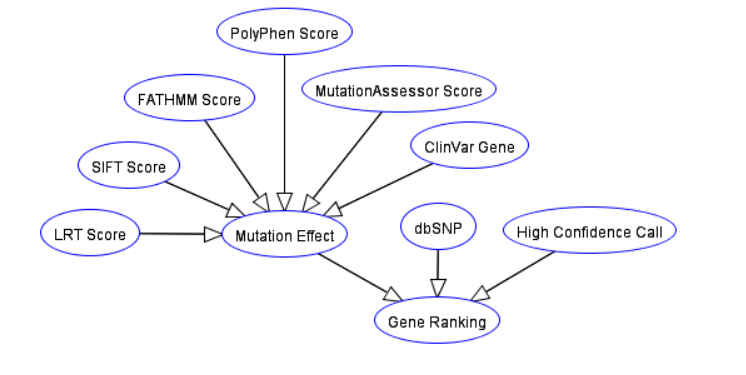
\includegraphics[width=\textwidth]{bayesiannetwork.png}
\caption{\textbf{Final Bayesian Network used in Analysis}}
\centering
\end{figure}
This network structure was chosen as we wanted to use three different sets of information to rank the importance of a variant, (i) the overall functional effect of the variant, (ii) the prevalence of the variant in the population and (iii) the confidence of the variant call.\\\\ Firstly, the functional effect of a variant should be key in determining its rank. This is important as the greater the functional effect, the more deleterious a variant will likely be. We used functional annotations from ANNOVAR (Wang, Li, \& Hakonarson, 2010) to predict the overall impact of variants via an ensemble of mutation effect predictors.  These predictors use different methods to predict the phenotypic effect of that variant, such as using position-specific substitution matrixes and Hidden Markov Models to predict the effect of an amino acid change on protein structure and function. Another functional annotation used was the ClinVar database, a curated repository of known human variants and their resulting phenotypes (Landrum et al., 2014). The output of these annotations are converted into probability scores and used to update the ranking of the variant (Table 3). 
\begin{table}[H]
\caption{\textbf{Functional Annotations obtained from ANNOVAR}}
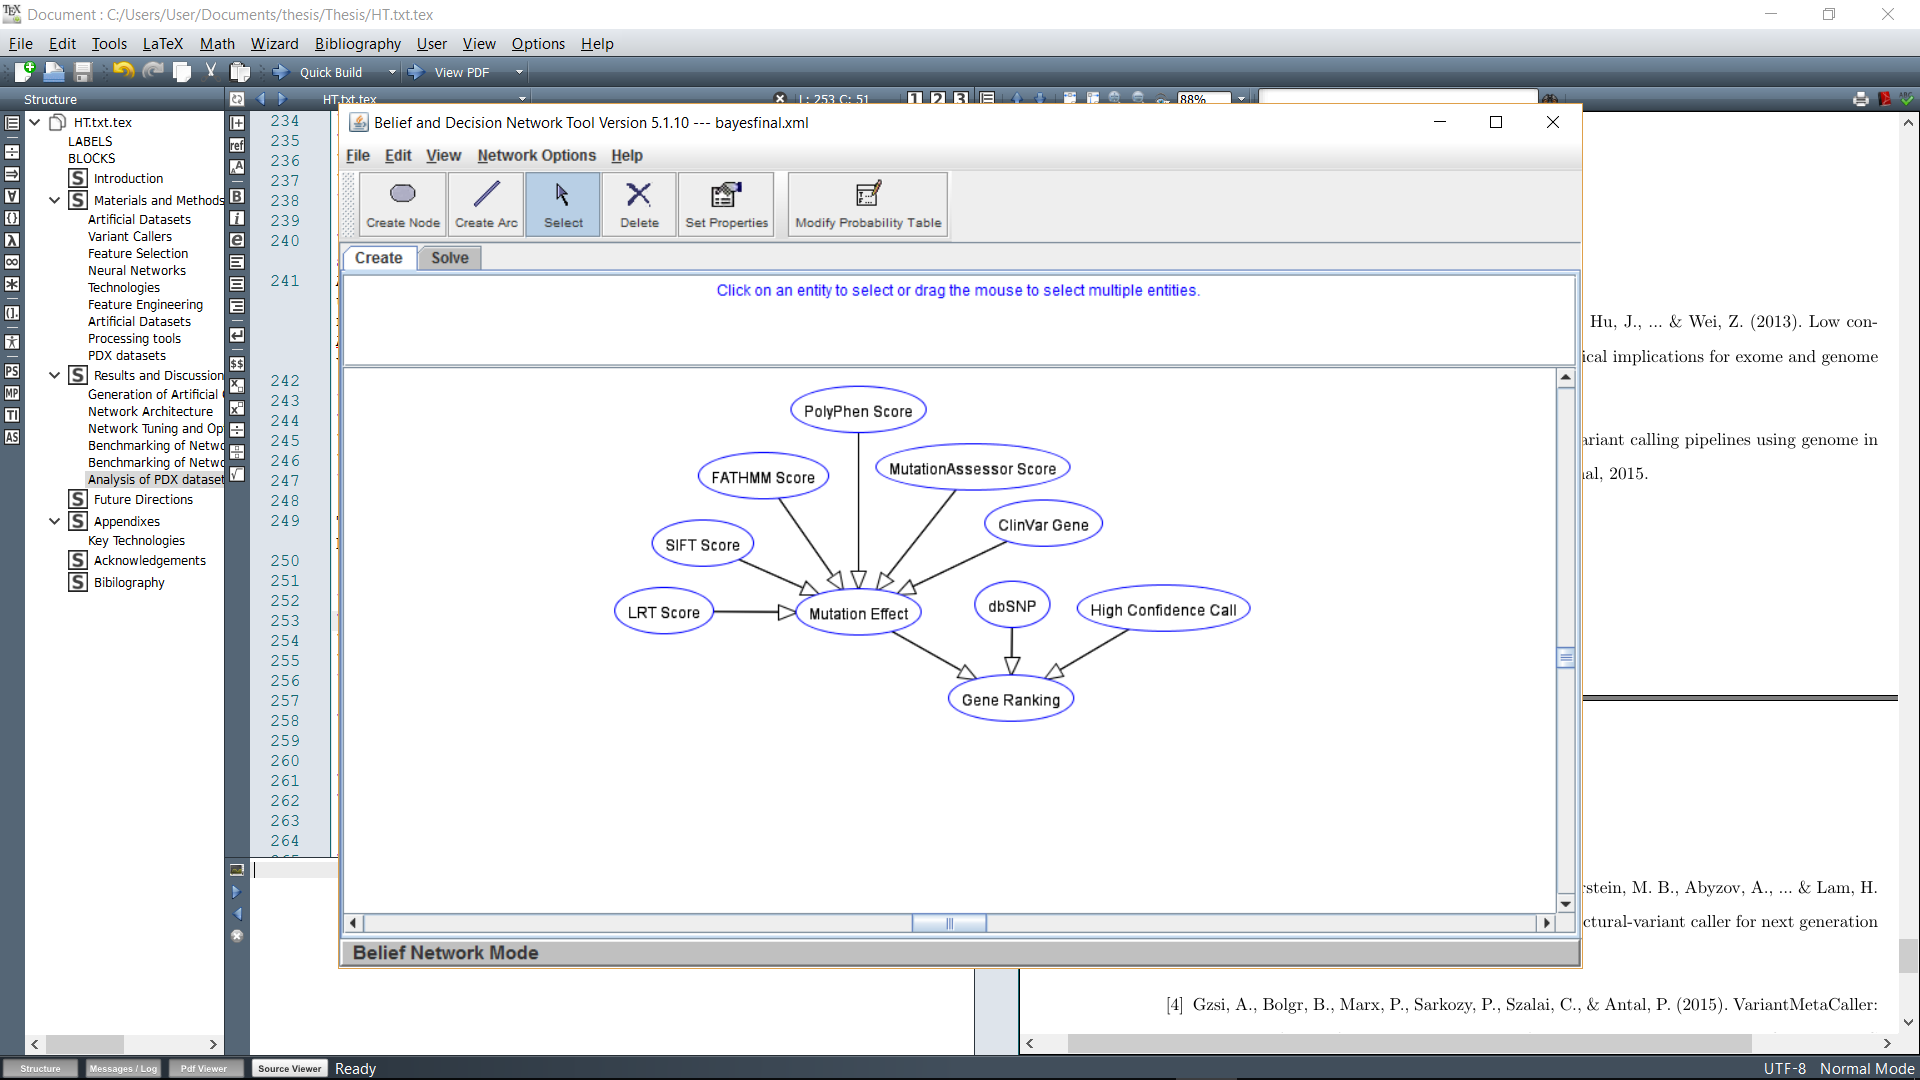
\includegraphics[width=\textwidth]{annovarfeatures.png}
\centering
\end{table}
Next, the prioritisation rank should also be determined by how common the variant is, which we can obtain by looking up known population single nucleotide polymorphisms (SNP). If the variant is labelled as an SNP, which is defined as a common polymorphism that is found in at least 1\% of the population, then its prioritisation should be lower. Evidence supporting this lower prioritisation for SNPs comes from population studies showing that common variants have lower odds ratios with diseases when compared to rare variants (Schork et al., 2009), and rare variants have been shown to be more important as drivers of disease than common variants (Cirulli \& Goldstein, 2010; Pritchard, 2001). Finally, the confidence of the variant call should factor into how important it is -- the more confidence we can have in a variant call, the more highly it should be prioritised. \\\\ Subsequently, we can use these probabilities to compute the final Bayesian probability ranking, which is shown in the equation below. Based on scores provided, we report the update the conditional probabilities using the probabilities chain rule -- for the first level; this is given as :\\
\begin{equation}
\begin{split}
P(Impt | (Func \ Eff  \ \cap \ Rare  \cap High\ Conf)) =  \frac{P(Impt \cap Func \ Eff  \ \cap \ Rare \cap High \ Conf )}{P(Func \ Eff  \cap Rare  \cap High \ Conf )}
\end{split}
\end{equation}
\tiny
\indent
P(Impt) refers to the probability of the gene being important,\\
\indent P(Func Eff) refers to the probability of the gene having a functional effect,\\ 
\indent P(Rare) refers to the probability of the gene being uncommon and\\  \indent P(High Conf) refers to the probability of the gene being a high confidence call.\\\\
\normalsize
\noindent
To compute the final probabilities, the software library Pomegranate was used. This simplifies the bayesian network drawing and probability computation of the final ranking scores (see Relevant Code -- Section 7.3).
\subsection{Validation of Bayesian Network Ranking on PDX dataset}
To study the effectiveness of our Bayesian network ranking system, we sequenced and analysed a patient-derived xenograft (PDX) tumour genome. This tumour genome was grafted onto a immunocompromised mouse from a patient with a known cancer subtype -- Diffuse Large B-Cell Lymphoma (DLBCL). We chose to test our Bayesian ranking system on DLBCL as it is a well-characterised disease model (Knudson et al., 2001; Alizadeh et al., 2000). After sequencing the DLBCL tumour genome, we identified high-confidence variants using the deep learning neural network, and then ranked these variants using the Bayesian network ranking method. Figure 22 shows the genes associated with top 30 variants ranked by probability of importance. 

\begin{figure}[H]
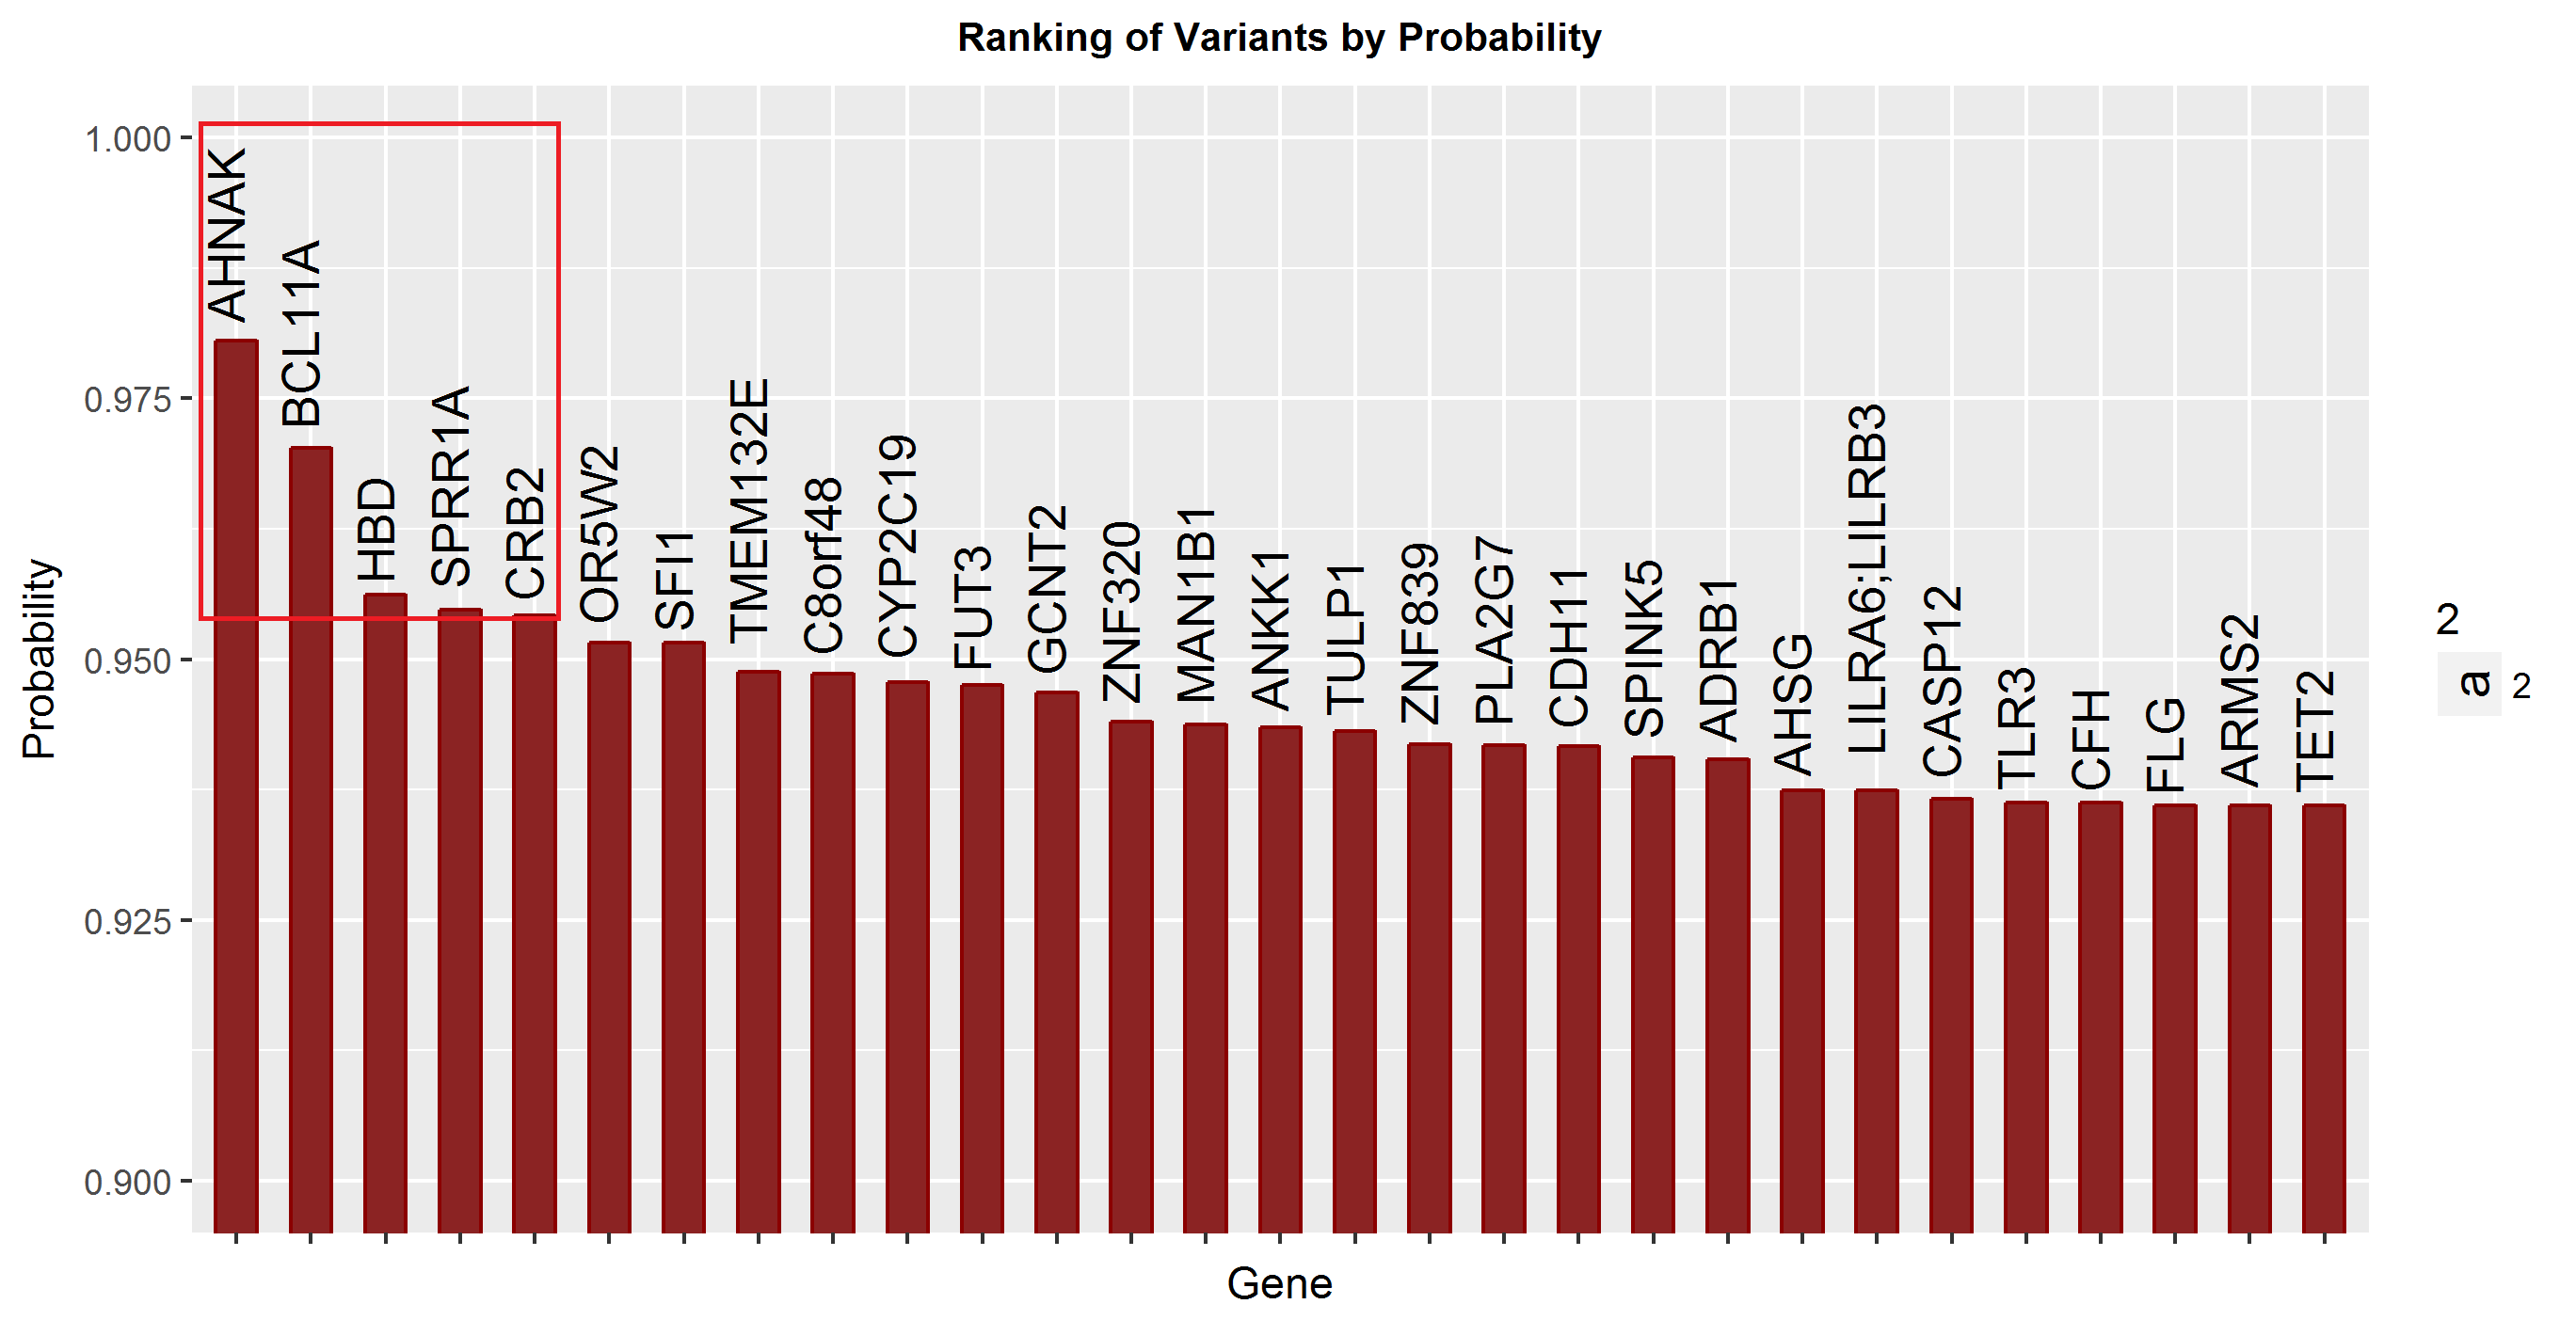
\includegraphics[width=\textwidth]{bayesianranks.png}
\caption{\textbf{Associated genes of top 30 Variants Ranked by Probability from Bayesian Ranking method}}
\centering
\end{figure}

Studying the top 5 genes, we found that four of these five genes have been implicated in lymphomas or other cancers (Table 4), which are AHNAK (Rank 1), BCL11A (Rank 2), SPRR1A (Rank 4) and CRB2 (Rank 5). \\\\  AHNAK is a known tumour suppressor and has been known to be downregulated in lines of Burkitt Lymphoma (Lee et al., 2014; Amagai et al., 2004; Shtivelman et al., 1992). BCL11A is a known proto-oncogene in DLBCL and has been found to be overexpressed in 75\% of primary mediastinal B-cell Lymphomas, a subset of DLBCL (Weniger et al., 2006; Satterwhite et al., 2001). SPRR1A, the fourth gene ranked in terms of importance, has been shown to be expressed in DLBCL (Zhang et al., 2014) and its expression has been shown to strongly correlate with 5-year survival rate (Figure 23). Finally, development of B-Cell lymphoma has been noted in CRB2 related syndrome, which is a bi-allelic mutation of CRB2 (Slavotinek, 2016; Lamont et al., 2016). Interestingly, the last highly ranked gene was the delta subunit of Hemoglobin (HBD). While there is no strong evidence for the role of Haemoglobin in DLBCL, it has been shown to be expressed in aggressive glioblastomas lines, which suggests a possible uncharacterised role for HBD in cancer (Emara et al., 2014). \\\\ In summary, the ability for the Bayesian network to prioritise four genes that are related to DLBCL and lymphomas gives us high confidence that the Bayesian ranking method can pick up important and relevant mutations. Without such a ranking system, we would have to look through over a multitude of genes, without a way to systematically compare their likelihood of importance. 
 
\begin{table}[H]
\caption{\textbf{Top Ranked Genes from Bayesian Ranking}}
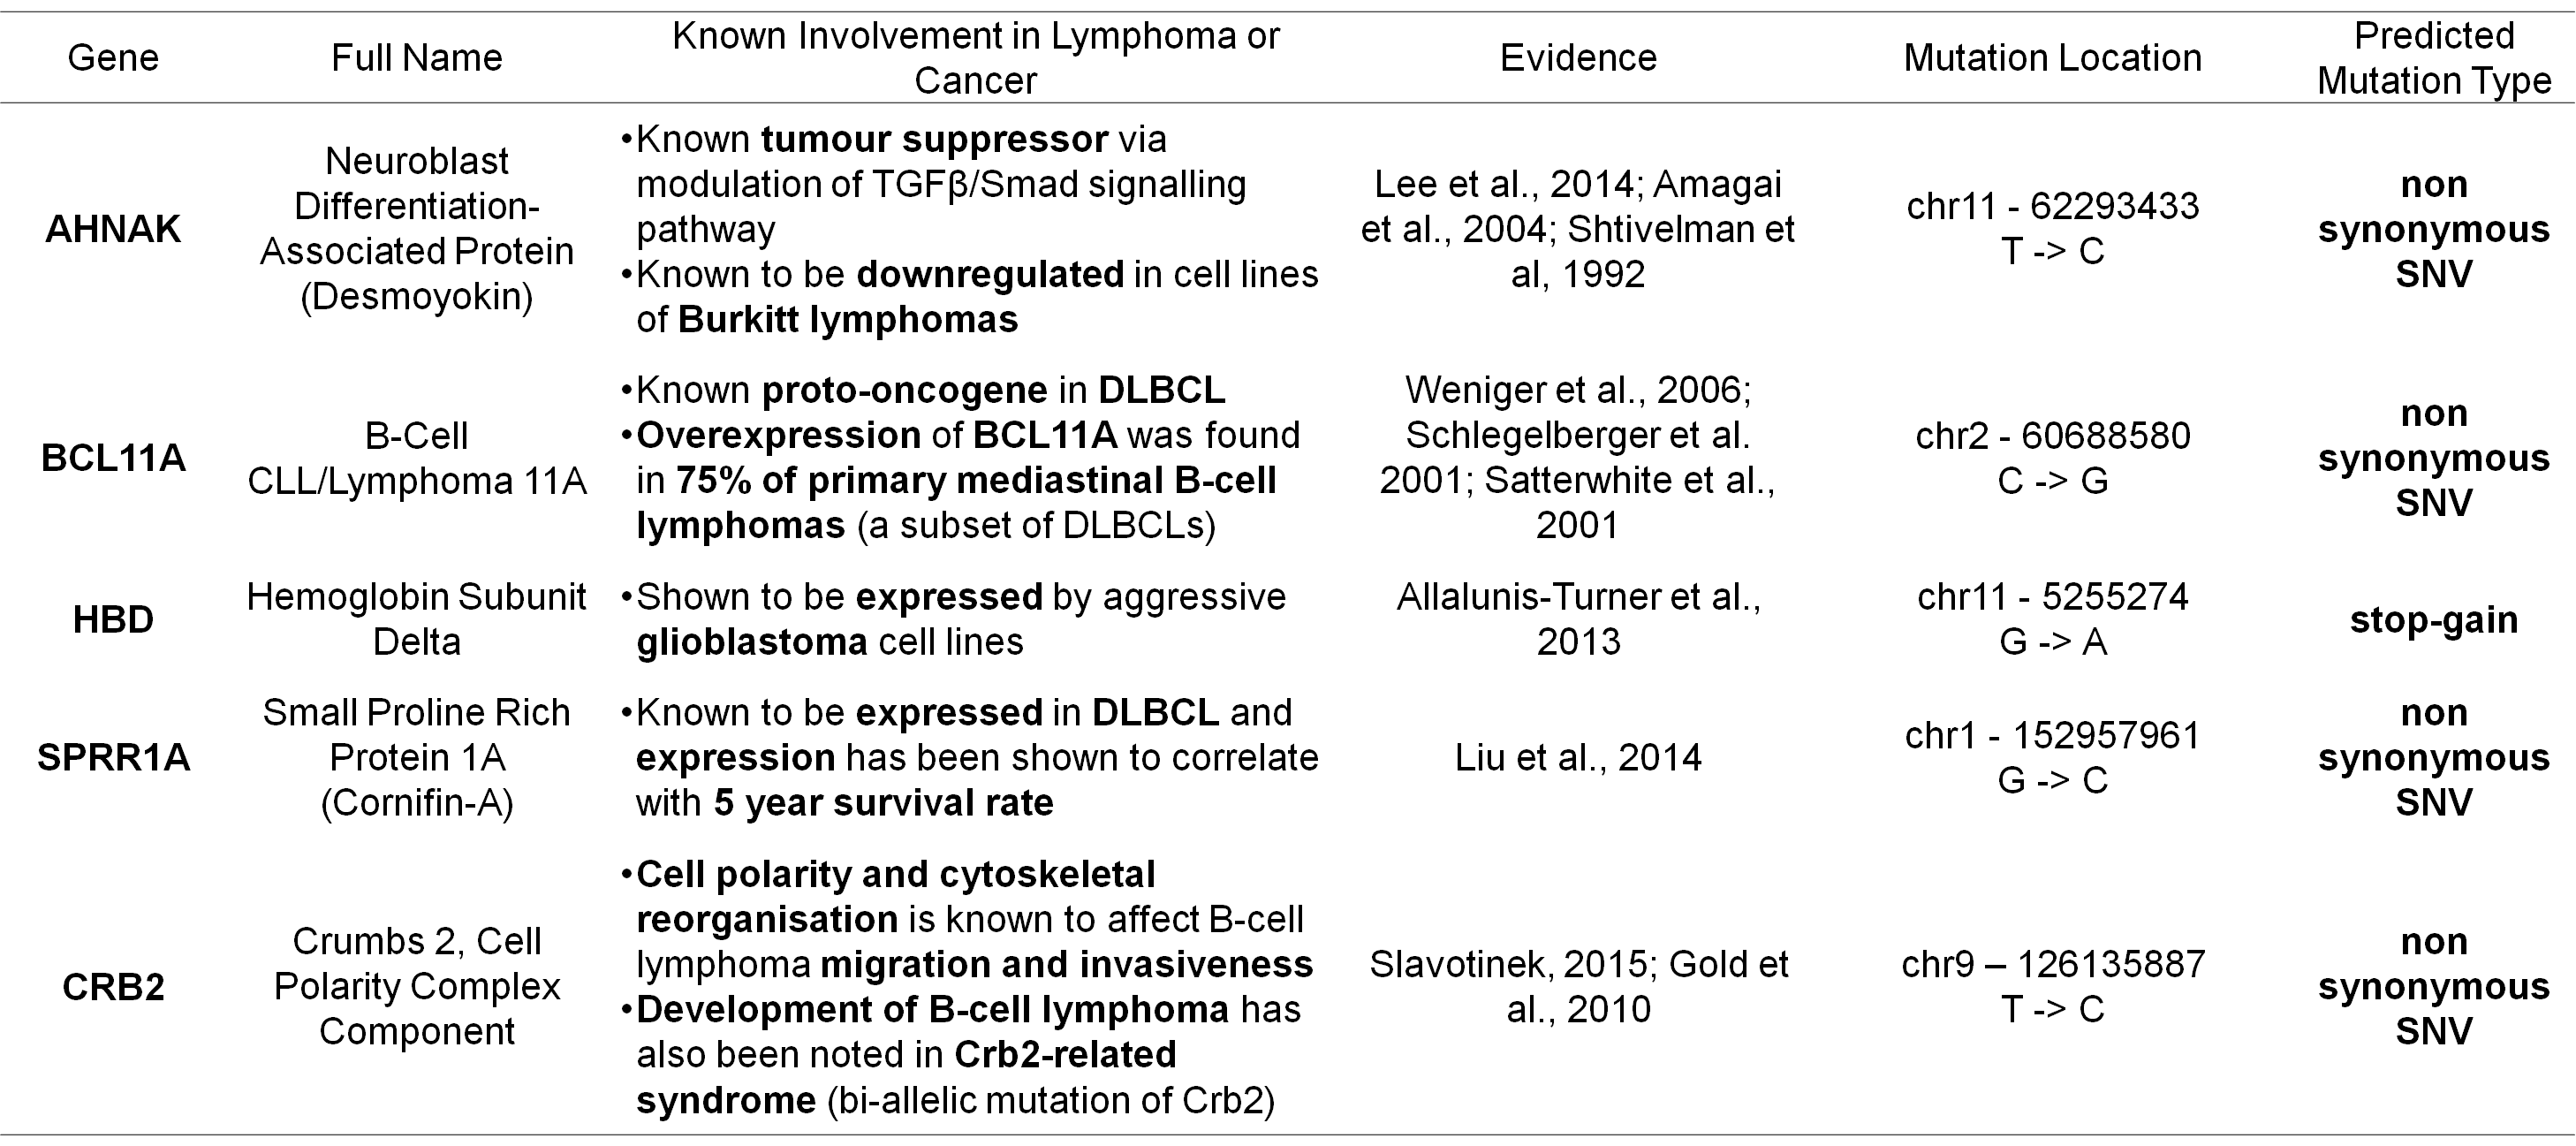
\includegraphics[width=\textwidth]{top5importantgenes.png}
\centering
\end{table}

\begin{figure}[H]
\centering
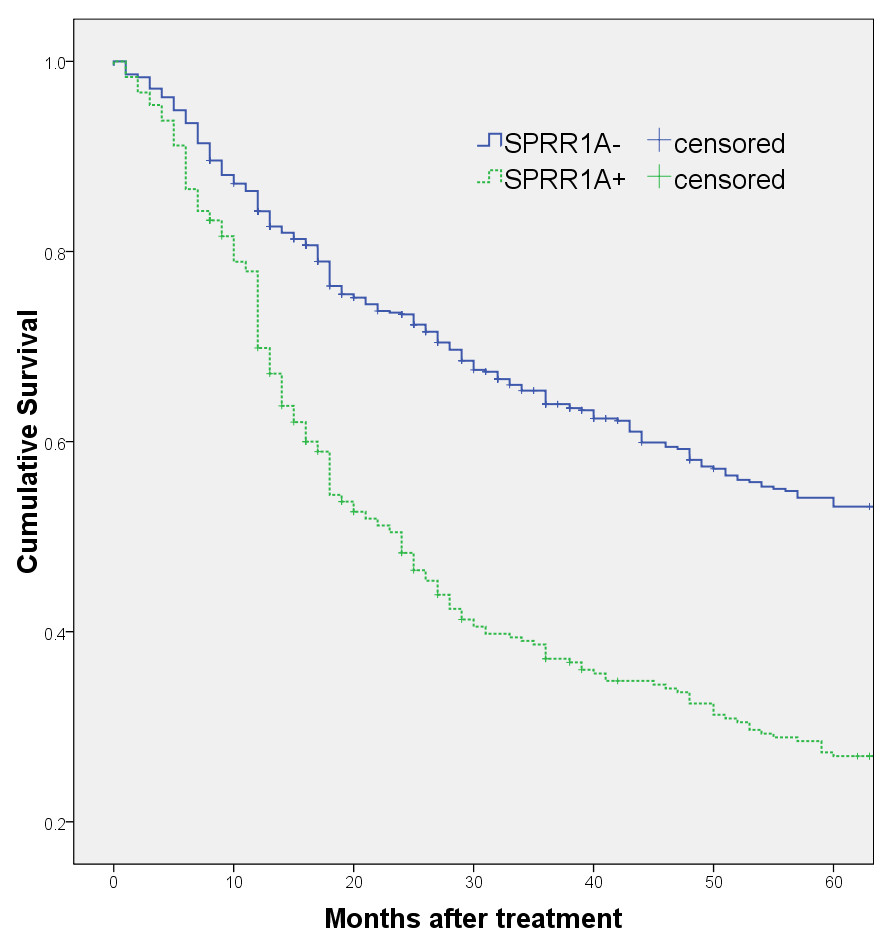
\includegraphics[width=0.5\textwidth]{sprr1adataset.jpg}
\caption{ \textbf{5 Year Survival Curve of Patients with SPRR1A positive and SPRR1A negative DLBCL.} Patients that were SPRR1A positive were noted to have a significantly lower 5 year survival rate than patients that were SPRR1A negative. Source : Zhang et al. (2014), Figure 2.}
\end{figure}


To aggregate the data from our Bayesian Ranking system, we designed a Circos plot to visualise the characteristics of the top 300 genes picked up by our gene ranking system (Figure 24).

\begin{figure}[H]
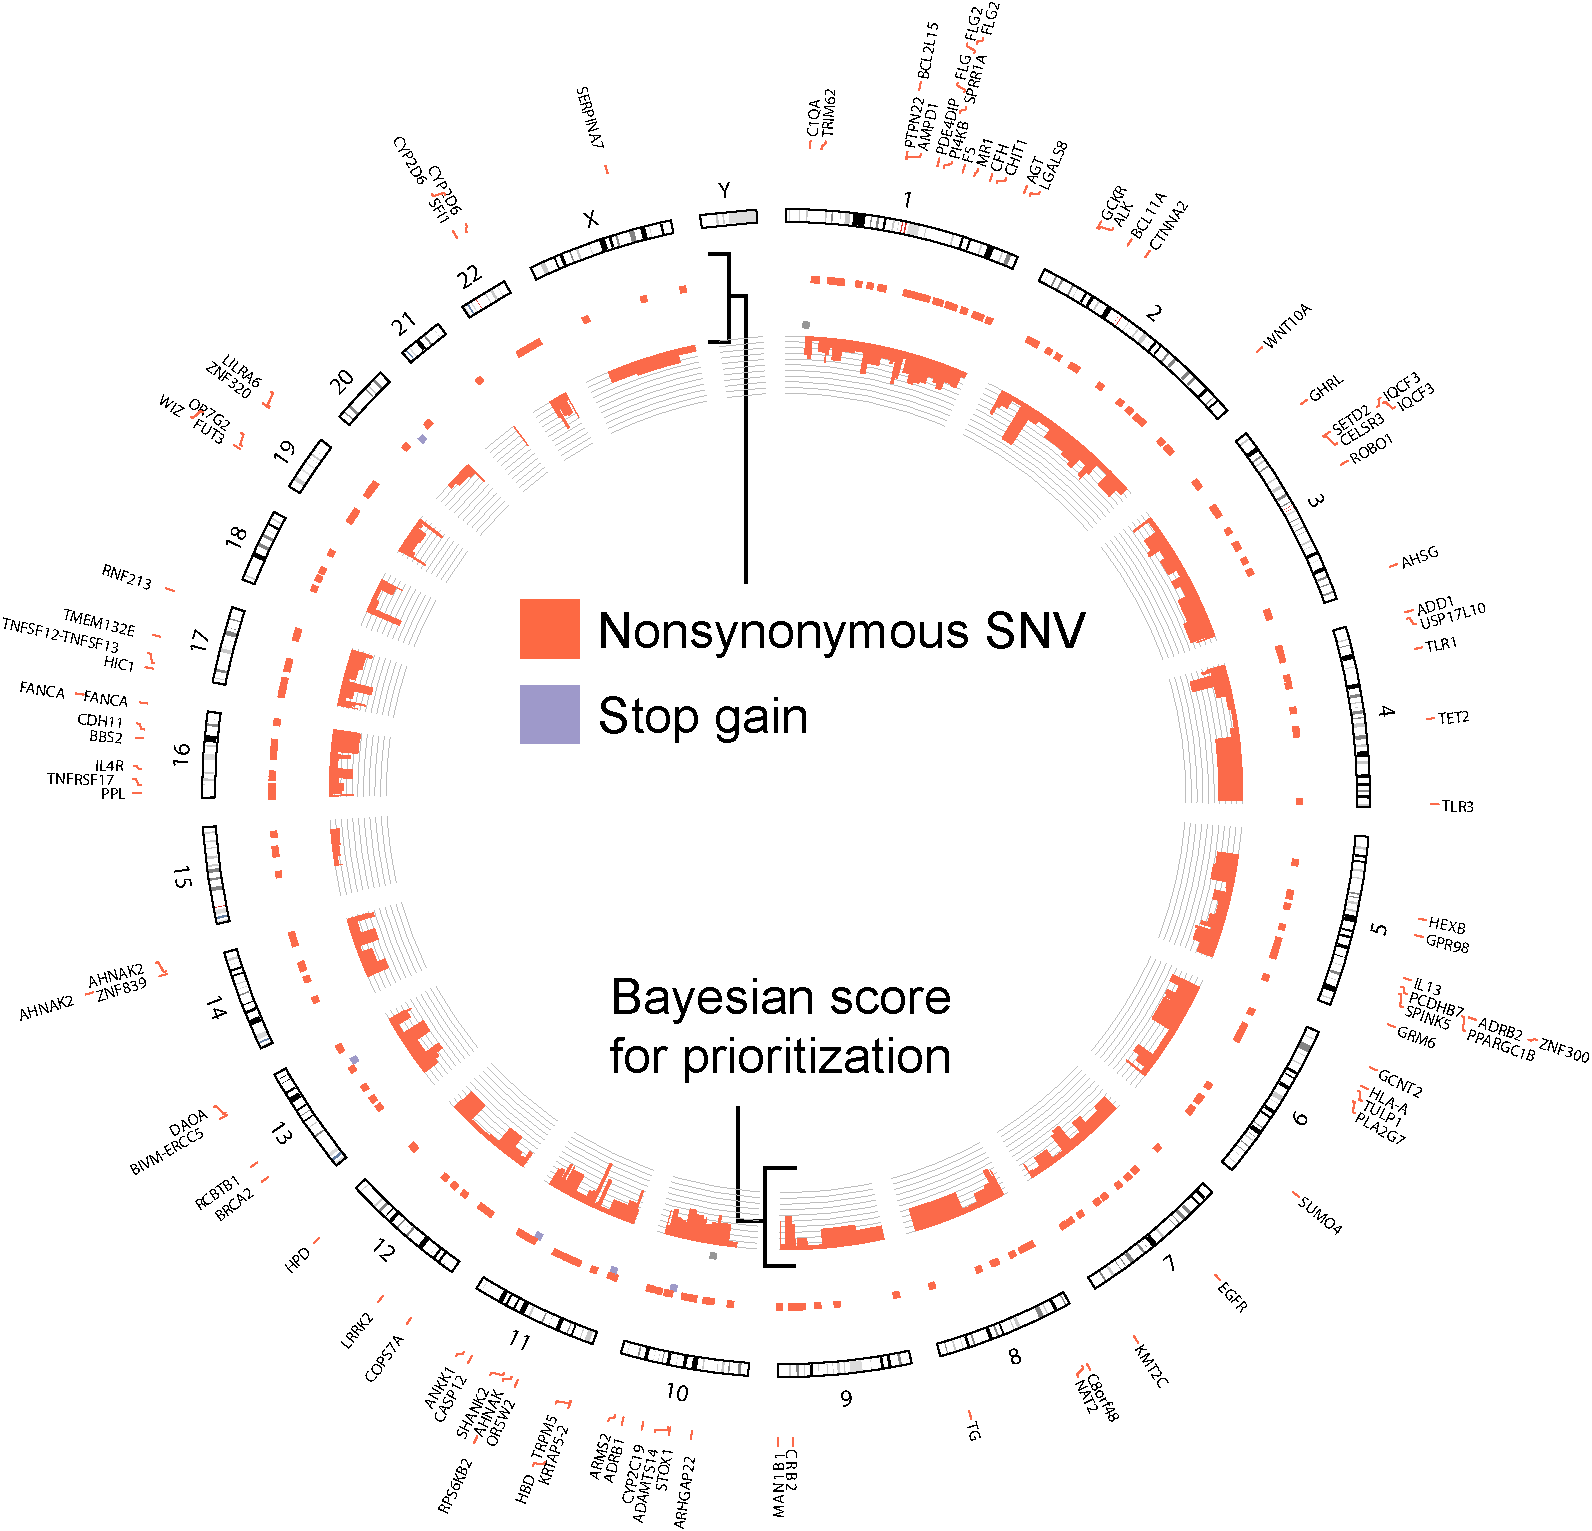
\includegraphics[width=\textwidth]{circosplot.pdf}
\caption{\textbf{Circos Plot of Top 300 Ranked Genes from Bayesian Network Ranking.} In this Circos plot, the outer track indicates the top ranked genes and their positions on the chromosome. The inner track describes the type of mutation that was observed -- most mutations were non-synonymous SNVs, with a few stop-gain mutations. The innermost track shows the relative probabilities of each ranked gene.}
\centering
\end{figure}

From the Circos Plot (Figure 24), we find several interesting gene families that might be relevant in DLBCL. These include two Toll-like receptors(TLRs), TLR3 and TLR1 (Chromosome 4), as well as two interleukin receptors, IL4R and IL1$\beta$ (Chromsome 2 and 16). TLRs are of significant interest in DLBCL because to their interaction with MYD88 (Yu, Wang \& Chen, 2012), which is a well-characterised oncogene in DLBCL (Kraan et al., 2013; Ngo et al., 2010). Interleukin receptors are also important in DLBCL due to their importance in mediating inflammation and immune response (Balkwill \& Mantovani, 2001), which is known to be affected in DLBCL (Monti et al., 2005). Thus, we show that our Bayesian network can be used by clinicians to quickly interrogate the information from functional annotations and database lookups to report important genes.

\newpage
\section{Discussion}
In this study, we sought to address the two major problems that limit the use of next generation sequencing in clinical genomics: (i) the identification of high-confidence variant calls; and (ii) the ranking of functionally important genes.\\\\
We demonstrate the validation of high-confidence variant calls using an optimised deep learning neural network on both real and simulated datasets, and we also show that a Bayesian network can rank and prioritise genes in a systematic way so as to obtain functionally important genes. Consistent with the validity of our approach, we show that four of the top five genes had published findings that linked them with B-cell lymphoma. Of the top 300 genes ranked, we also found families of genes that are known to be involved in lymphoma progression, including the Toll-like receptor and interleukin receptor families. 







\subsection{Adapting Deep Learning for Improving Variant Calling Accuracy}

Deep learning networks have been used successfully to solve complex non-linear problems (Sun et al., 2014; Lusci et al., 2013). In this study, we demonstrate that a deep learning architecture can be used to integrate complex features from an ensemble of variant callers to improve variant calling accuracy. We found that not all network architectures were suitable for processing the complex features. When a typical flat network architecture was used, the network was unable to converge and learn, suggesting that the number of features was too high for optimal learning. Interestingly, when the number of features was compressed using PCA, a commonly used dimensionality reduction algorithm, the flat network was still unable to learn, indicating that compression of features did not play a major role for the performance of flat networks.\\\\
Because the straightforward application of flat networks did not work well, we reasoned that the complex features represented multimodal data that could not be represented properly in the flat input layer (Eitel, 2015; Suk, Lee \& Shen, 2014). Consistent with this hypothesis, we developed a merged network architecture that comprised of subnets for features of each variant caller that were subsequently merged into a common network for variant call prediction.\\\\
When the merged architecture network was further optimized by varying the network layers, gradient descent optimizers and sample balancing, we did not observe any significant improvements in the variant calling performance, suggesting that the merged architecture for multimodal data was the most significant contributor to the ability of the network to learn from an ensemble of variant callers.\\\\
Using our optimised merged network architecture, we were able to call variants more accurately than single or concordant variant callers, with F1 score improvements of 6\% in simulated datasets and 4.5\% in the NA12878 dataset. Although several ensemble methods have been proposed such as VariantMetaCaller and BAYSIC (Gézsi et al., 2015; Cantarel et al., 2014), the performance metrics reported were not directly comparable to the F1 scores used in this study. It would be of interest to implement a pipeline with all the ensemble methods in a common framework to enable proper comparisons of the variant calling performance.

\subsection{Improving Performance of Deep Learning Approach}

Although the deep learning network was able to improve the accuracy of variant calling, there are several areas worth looking into that would likely improve their performance. This includes increasing the number of input features, as well as generating real-world datasets with established ground truth variant calls.\\\\
Firstly, deep learning networks, like any machine learning algorithm, are highly dependent on the features used in the input layers for pattern identification and prediction. In our study, we chose five variant callers that are commonly used and correspondingly the features are limited by the outputs provided by each variant calling algorithm. The inclusion of other orthogonal features from alternative variant callers and alignment tools may provide additional data that can improve prediction accuracy.\\\\
Secondly, the accuracy of the deep learning network is also highly dependent on the training datasets. In this study, we trained the optimised network using the NA12878 dataset which includes a set of high confidence calls from the integration of calls from several orthogonal sequencing technologies. However, as the ground truth calls in the NA12878 are also subjected to noise and biases from sequencing, it is likely that some ground truth calls may have been misclassified, leading to false positive and false negative calls. Indeed, Zook et al.(2014) estimate a possible false negative or positive for every 30 million bases in the NA12878 dataset. To address this problem, several ongoing efforts are focused on obtaining verified truth variants by Sanger sequencing, which remains the gold standard for identifying prevalent mutations (Tsiatis et al., 2014). The establishing of verified variants would provide a training set that would be a major step in improving the accuracy performance of a deep learning network.
\subsection{Improvements to Bayesian Network}
In this study, we used a Bayesian model to rank important genes from a DLBCL sample. Encouragingly, we found that four of the five top ranked mutations were linked to B-Cell lymphoma, indicating that the validity of a Bayesian network approach to identify functionally important genes. Furthermore, we were able to find important receptor families linked in DLBCL, such as Toll-like receptor and interleukin receptors in the highly ranked genes, providing further evidence for the use of a Bayesian network in gene prioritisation. \\\\
However, our Bayesian network is limited by the lack of a gold standard to benchmark the methods. In deep learning, we could validate our results using simulated datasets where the ground truth variants are known and the NA12878 dataset where high confidence variants is known. However, for the Bayesian network, we can only infer the validity of such a system by looking at the top ranked genes and confirming their importance. To obtain such a gold standard, in-depth functional analysis into the gene, mRNA and protein expression profiles would have to be done. \\\\
A second key limitation in such a Bayesian network is the setting of prior probabilities and conditional probabilities for discrete variables. While the usual strategy is to study the datasets to obtain prior conditional probabilities, we cannot obtain the ground truth of how important a gene is functionally, and thus we have to make assumptions so as to define the probabilities.\\\\
One last limitation is that in our current network structure, the effect of a mutation (functional effect), the prevalence of the SNV and the confidence of a variant call are equally ranked. However, with this network structure, a high confidence mutation that is not functionally relevant could be prioritised over a lower probability but more functionally relevant mutation. Since we are chiefly concerned in the functionally important genes, the network structure might not be the most suitable for predicting the most important genes. One potential improvement is to study how the hierarchy can be altered - specifically to see if the high-confidence node could be used as a prior probability to all the other nodes, which reduces its overall importance in the probabilistic model.
\subsection{Clinical Usage of Bayesian Networks in Gene Prioritisation}
We specifically chose the Bayesian Network structure as it presents a clear and understandable predictive models that clinicians are able to use, along with other tools like gene panels (Olek and Berlin, 2002) or simply doing literature reviews. 
While gene panels work well in a clinical setting, Bayesian Networks have the added advantage of not being limited to a specific set of genes. This allows doctors to find other similar proteins or interacting agents that might be related to the known deleterious genes and use that information in their treatment and diagnosis (Meldrum et al., 2011).\\\\
However, one limitation in implementing such a Bayesian network is that all the information that goes into it has to be manually curated. Because it taps upon previously curated databases, it is limited in scope to the pre-processed information it already contains. One possible alternative to solve this problem is to develop a data miner to mine the literature for possible relationships between genes and diseases, thus creating a self-updating database. However, this is currently difficult to implement because a machine would have to learn the complex conceptual relationships between genes and phenotype, and this is currently an unsolved problem (Cambria \& White, 2014). Furthermore, such a system would require still human intervention to verify the data being mined is valid and appropriate. Ultimately, this should still be a useful tool as it allows for an interface for clinicians and researchers to easily share and obtain information, and a single clinician to tap upon the expertise and data from many different research institutions without having to manually sieve through the literature. 

\subsection{Future Directions}
There are several avenues that the integrated deep learning and Bayesian network analysis could be extended to improve the performance and utility.
\begin{enumerate}
	\item To improve the performance of the deep learning network, additional features from other variant caller could be included in the pipeline to provide more orthogonal data for prediction accuracy. In addition, the network could be trained on additional real datasets with ground truth variant calls so that the network is able to generalize and predict high confidence variant calls on a wide range of datasets.
	\item The Bayesian network could be extended to integrate information about druggable gene and variants using a drug-gene interaction database such as DGldb (Griffith et al., 2013). This would enable the prioritisation of mutations which have possible candidate drug targets. 
\end{enumerate}
\subsection{Conclusion}
In this study, we have shown the use of deep learning neural networks to validate variants in both real and simulated datasets successfully. We also show that using a Bayesian network can identify important genes within a lymphoma disease sample. Ultimately, we hope to be able to put these networks to use in a clinical setting to augment treatment and diagnosis of diseases.


\newpage
\section{Appendixes}

\subsection{Neural Network Learning}
Machine learning with deep neural networks is underpinned by two key phases, the feed-forward phase and the backpropagation phase. 
\subsubsection{Feedforward Phase}
The feedforward phase describes the computation of a prediction, and during this phase, the input features are used to compute the final output prediction. For a simple network below:
\begin{figure}[H]
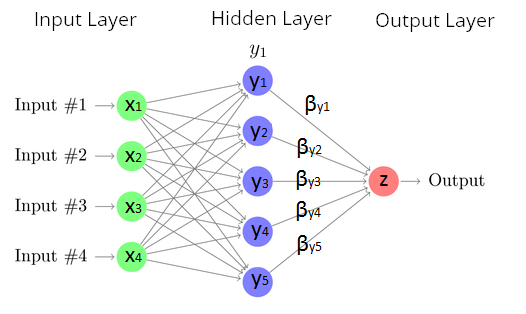
\includegraphics{neuralnetworksample.png}
\caption{\textbf{Sample Neural Networks with Labelled Nodes and Weights.}}
\centering
\end{figure}
The final prediction, z is computed with the equation:
\begin{equation}
z = \beta_{y1} * y_1 + \beta_{y2} * y_2 + \beta_{y3} * y_3 + \beta_{y_4} * y_4 + \beta_{y_5} * y_5
\end{equation}
Where $\beta$ indicates, the weights linking each output to the input of z and each of the $y_i$ terms are computed in the same manner from the $x_i$ layer. At each node (x,y,z), there is also the existence of an activation function that modifies the input of the node to compute an output. Commonly used activation functions include the rectified linear unit (ReLU), sigmoid functions like hyperbolic tangent and logistic function,$ S(T)=\frac{1}{1+e^{-t}}$.Thus, the final prediction can be seen as a summation of all weights multiplied by the activation output of each node. In theory, we can expand each of the $y_i$ terms in equation (2) to include the $y_i$ layer activation function as well as rewrite the $y_i$ layer inputs in terms of the sum of outputs and weights from the $x_i$ layers. This complex integration of terms allows for the neural network to form complex continuous decision boundaries as the neural networks can compute sophisticated non-linear prediction functions despite being a fundamentally linear model.
\subsubsection{Backpropagation Phase}
After a prediction is made, we then have to check whether it is correct and change our weights if an erroneous prediction was made (Figure 26).
\begin{figure}[H]
\centering
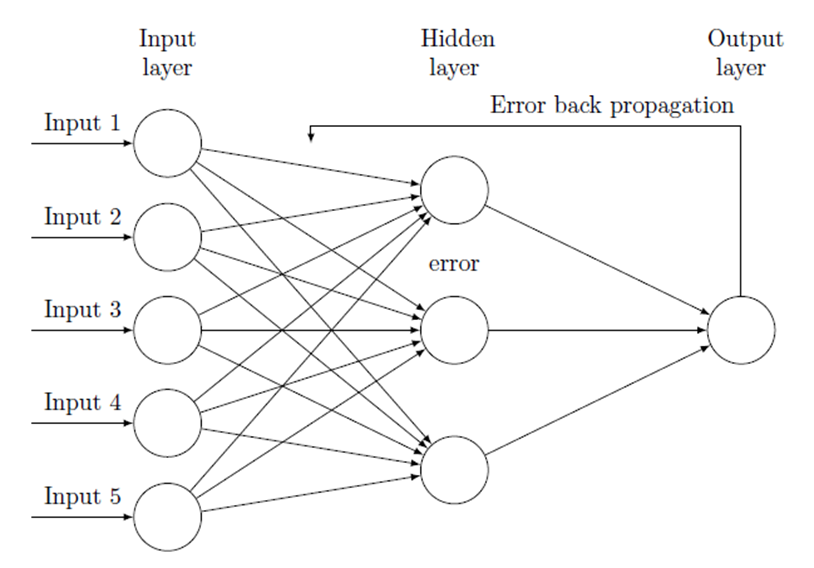
\includegraphics[width=0.8\textwidth]{backpropagation.png}
\caption{\textbf{Backpropagation of Error Terms}}
\end{figure}
This is the backpropagation step, which involves backpropagating the error terms from the output layers to the input layer and updating the weights at each node based on the differential relationship between the error and each specific gradient. Specifically, this is governed by the optimiser functions which have been mentioned earlier -- one example of such a function is the Stochastic Gradient Descent function, which is 
\begin{equation}
\beta^n_{yi} = \beta^{n-1}_{yi} - \alpha \frac{\partial{E_n}(\beta)}{\partial{\beta_i}}
\end{equation}
Here, each $\beta$ term indicates a gradient, $\alpha$ is a constant for the learning rate and $\frac{\partial{E_n}(\beta)}{\partial{\beta_i}}$ is the term used to modify the weight of the gradient based on the cost function ${E_n}(\beta)$. The idea used in all backpropagation functions is gradient descent, where the contribution of the gradient term to the error is computed, and the gradient is changed by an amount in order to reduce the future contribution of the gradient to that error. 
\subsubsection{Cost Function in Gradient Descent}
Here it is useful to consider what the cost function ${E_n}(\beta)$ is. It is essentially the error rate when a set of gradients is used to perform predictions, as it measures how many accurate predictions were made and how many wrong predictions were made. For a binary class predictor (which is what we are using, only true and false), this is given by the equation
\begin{equation}
E(\beta) = - \frac{1}{n}\sum_{i=1}^{n}{\sum_{j=1}^{2}y_{ij}log(p_{ij})}
\end{equation} 
where $y_{ij}$ indicates the empirically observed probabilities of each class label while $log(p_{ij}$ is the theoretical probabilities of each class label. This is also known as binary cross-entropy, which is derived from Shannon's entropy (See Appendix 5.2.1). From this term, we see that if the neural network predicts something with a high probability ($y_{ij}$ is high) and it is false ($p_{ij}$ is low) so then $log(p_{ij})$ is a big negative number, and so the cost function will very high. On the other hand, if $y_{ij}$ and $p_{ij}$ is high then the entropy will be close to zero, indicating a correct prediction. Since each of the prediction terms can be rewritten in terms of the gradient(rewrite z in terms $\beta y_i $ and so on), we can theoretically compute the contribution of each gradient to the cost function to see how the cost function changes as the gradient changes. Thus, this is what gradient descent does -- it tries to see how the cost function changes as each gradient changes, then attempts to move the gradient in the direction that minimises the error term.

\begin{figure}[H]
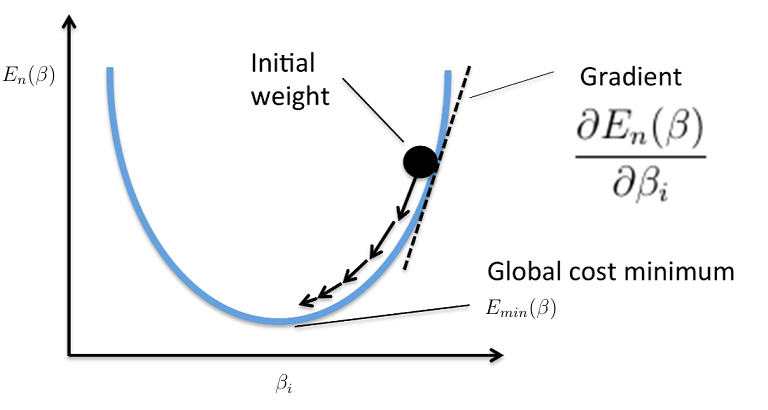
\includegraphics[width=\textwidth]{gradientdescent.png}
\caption{\textbf{Graphical Illustration of Gradient Descent.} Gradient descent attempts to find the gradient at which the cost function is minimised (since the cost function depends on the gradient).}
\centering
\end{figure}
 This is best seen in Figure 27 above, where the gradient or specifically the partial differentiation of the cost function with regards to each gradient is used to move the gradient to a new position so as to minimise the error term. Thus, machine learning is, in essence, a minimisation problem -- we want to find a set of weights that minimises the cost function. Because the cost function describes how many predictions we made correctly, gradient descent essentially trains our network to accurately predict outputs from inputs.

\newpage
\subsection{Feature Engineering}
We subset our features into three broad sets, which are base-specific information, sequencing error and bias information features, and calling and mapping quality. \underline{Base information} tells us base specific properties, including information contained in the base as well as the quality of sequenced bases in the samples. \underline{Sequencing error and bias} features attempt to tease out potential biases in sequencing, including features such as GC content, longest homopolymer run and as well as allele balances and counts. Finally, \underline{calling and mapping quality} provides information on the mapping and calling confidence of the variant callers, and includes features such as genotype confidence and mapping quality. In all, these sets of information provide information on the key aspects of variant calling -- specifically the properties of the bases in the samples, the characteristics of the sequencing process and finally the variant calling and mapping algorithms.\\\\
\subsubsection{Base Information}
\underline{Shannon Entropy}\\
Shannon Entropy captures the amount of information contained in the allele sequences. It is calculated using the equation:
\begin{equation}
H(X) = -\sum_{i=1}^{n}P(x_i)\log_{2}P(x_i)
\end{equation}
where $P(x_i)$ is the probability of finding each base at each position. Thus, we calculate the entropy by summing up the probabilities/log(probabilities) at each position. This prior probability is calculated in two ways, and both are used as features -- firstly, the overall genome base probabilities are calculated over the entire genome, and thus the entropy is related to the probability of finding a base at any position in the genome. The second way prior probability is calculated is to take a region of space around the allele (10 bases plus the length of the allele in our calculations) and use those probabilities to calculate the entropy of the allelic sequence. Intuitively, it attempts to find out the amount of information contained within the allelic sequence, and hopefully, the neural network can use the information to determine the validity of a mutation.\\\\
\underline{Kullback Leibler Divergence}\\*
The Kullback-Leibler Divergence feature is similar to Shannon entropy, but instead, we use this to measure the informational change converting from the reference to the allele sequence. The Kullback-Leibler Divergence is calculated as follows:
\begin{equation}
D_{KL}(P||Q) = -\sum_{i=1}^{n}P(x_i)\log_{2}{\frac{P(x_i)}{Q(x_i)}}
\end{equation}
where $Q(x_i)$ is the prior probability of finding each base at each position based on the genomic region around the allele, while $P(X_i)$ is the posterior probability of finding a specific base inside the allelic sequence. Thus, the KL divergence describes the informational gain when the probabilities from Q is used to describe P. Intuitively, since we know the base probabilities of the region, we can then study the probabilities observed in the reference allelic sequence and see how well $Q(X_i)$ probabilities can approximate $P(X_i)$ probabilities.\\\\
\underline{Base Quality}\\
Base quality refers to the Phred score probability that the called allele is wrong. It is given by the equation:
\[ \scalebox{1.2}{$P=10^{\frac{-Q}{10}}$} \]
Where P is the Base Quality, and Q is the probability that the allele called is wrong. This is a number computed by the sequencing machine based on the quality of the base samples provided, and tells us how much confidence the sequencing machine has in calling that base.\\\\
\subsubsection{Sequencing Biases and Errors}
\underline{GC content}\\
This feature computes the calculated GC content of reference genome, which may affect sequencing results and accuracy as regions with a GC content are known to be more difficult to sequence. This is because of the greater strength of GC bonds, resulting in errors and biases in sequencing (Benjamini \& Speed, 2012).\\\\ 
\underline{Longest homozygous run}\\*
Homopolymer runs (AAAAAAAA) are known to cause sequencer errors (Quail et al.,2012), and might be a factor in determining whether a variant is true. This because long homopolymers provide the same type of signal to the sequencing machine, resulting in a difficult in estimating the magnitude of the signal or rather how many bases are in that homopolymer, resulting in errors and wrongly called variants. The reference sequence region including the allele was checked for homopolymer runs. \\\\
\underline{Allele Count}\\
Allele count gives the total number of alleles in called phenotypes. This feature provides information of possible biases in the sequencing machine.\\\\
\underline{Allele Balance}\\
Allele Balance describes the ratio of final allele called over all other alleles called(reference allele for heterozygous calls, or other alleles for homozygous calls). This feature give us information of possible biases in the sequencing machine. \\\\
\underline{Allele Frequency}\\
Allele Frequency describes the ratio of final allele called over all other alleles called(reference allele for heterozygous calls, or other alleles for homozygous calls). This feature give us information of possible biases in the sequencing machine. \\\\
\subsubsection{Calling and Mapping Qualities}
\underline{Genotype Likelihood}\\
The genotype likelihood provides the Phred-scaled likelihood scores of how confident the caller is in determining that it is a homozygous or heterozygous call, and for the homozygous calls whether it is a more likely to be a bi-allelic mutation or no mutation at all. This feature thus gives us the confidence of the caller in determining if one or two alleles have mutated. \\\\ 
\underline{Read Depth}\\
Mapped read depth refers to the number of bases sequenced and aligned at a given reference base position. The read depth tells us how many reads contributed to a specific call, and thus provides information on how much evidence there is for the variant call\\\\
\underline{Read Depth, 4 Variables}\\
This feature is a refinement of Read Depth, and provides 4 variables for the number of forward reference alleles, the number of reverse reference alleles, the number of  forward non-ref alleles and finally the number of reverse non-reference alleles.\\\\
\underline{Allele Depth}\\
This feature is a refinement of Read Depth, and describes the number of alleles supporting the variant call.\\\\
\underline{Quality by Depth}\\*
Quality by Depth is computed by dividing the quality score against allele depth, to obtain an average score of allele quality. This composite feature provides information on the information provided by each read supporting the call\\\\
\underline{Mapping Quality}\\
Mapping quality is originally a score provided by the alignment method and gives the probability that a read is placed accurately. The variant callers compute an overall mapping quality of the reads that provide evidence for a variant call which is given in this feature. A low mapping quality means that there are multiple positions where the reads contributing to this variant call could have gone, and thus providing evidence that this might not be an accurate call due to poor mapping.\\\\
\underline{Mapping Quality of Observed Reference Alleles}\\
This feature is a refinement of Mapping Quality, and describes the mapping quality of observed reference alleles.\\\\
\underline{Mapping Quality of Observed Alternate Alleles}\\
This feature is a refinement of Mapping Quality, and describes the mapping quality of observed alternate alleles.\\\\
\newpage
\subsection{Mathematical and Statistical Tools}
\subsubsection{Derivation of F1 Score}
The F1 score is a useful measure as it can measure both the precision as well as the recall of a predictor. For a binary predictor with a binary truth class(Figure 28), we can obtain four types of results -- true positives, true negatives, false positives and false negatives. 
\begin{figure}[H]
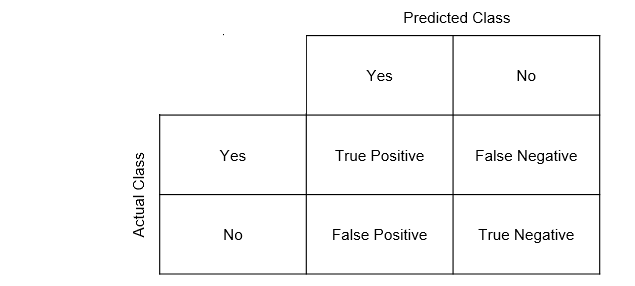
\includegraphics[width=0.8\textwidth]{confusionmatrix.png}
\caption{\textbf{Confusion Matrix for a Binary Class Predictor.}}
\centering
\end{figure}
True positives are positive predictions that are made that are positive class labels, while false positives are positive predictions that are made that have negative class labels. Similarly, true negatives are negative predictions that have negative class labels, while false negatives are negative predictions that are positive class labels. From this, we can define two equations, precision and recall. Precision is defined as (8) while recall is defined as (9). 
\begin{equation}
Precision = \frac{True \ Positive}{True\  Positive + False \ Positive} 
\end{equation}
\begin{equation}
Recall\ \ \ \ = \frac{True\ Positive}{True \ Positive + False \ Negative} 
\end{equation}
Precision tells us how likely a positive prediction made will be true, while recall tells us how much of the truth class positive predictions the predictor can classify successfully . Thus, a predictor can have a high precision but low recall (makes few predictions but are very accurate) or a high recall and low precision(makes many predictions that capture all truth variables, but have a lot of false positives as well). In genomics, both types of errors are not desired -- we would want all the predictions to be true (precision), while not losing out on any important mutations (recall). Thus, we use the composite metric, the F1 score, that looks at the overall precision and recall of a predictor. It is defined as follows:
\begin{equation}
{F1} \ Score \ \ \  \ \ = \frac{2*Precision*Recall}{Precision + Recall} 
\end{equation}
\\
\subsubsection{Principal Components Analysis (PCA)}
Principal Components Analysis (PCA) is a commonly used tool for dimensionality reduction. It was first proposed by Pearson in 1901 (Pearson, 1901) and has been commonplace in many data analytics and signal processing methodologies (Jolliffe, 2002). PCA works by attempting to discover orthogonal principal components (PCs) that are able to represent the original data. Specifically, this means that the PCs can capture variance in the datasets. This is done by finding the Eigenvalues and Eigenvectors of the dataset, with the eigenvectors representing a linear combination of all input variables and the eigenvalues representing the amount of variance that that eigenvector can represent. Ultimately, we select n eigenvectors that can represent a percentage of variance in our dataset. Because each eigenvector is orthogonal, they can capture the variance in the dataset.\\\\ For our analysis, we decided to use eight principal components -- we took the limit as the last principal component that was able to represent at least 0.5\% of the variance in the dataset (Figure 29).
 
\begin{figure}[H]
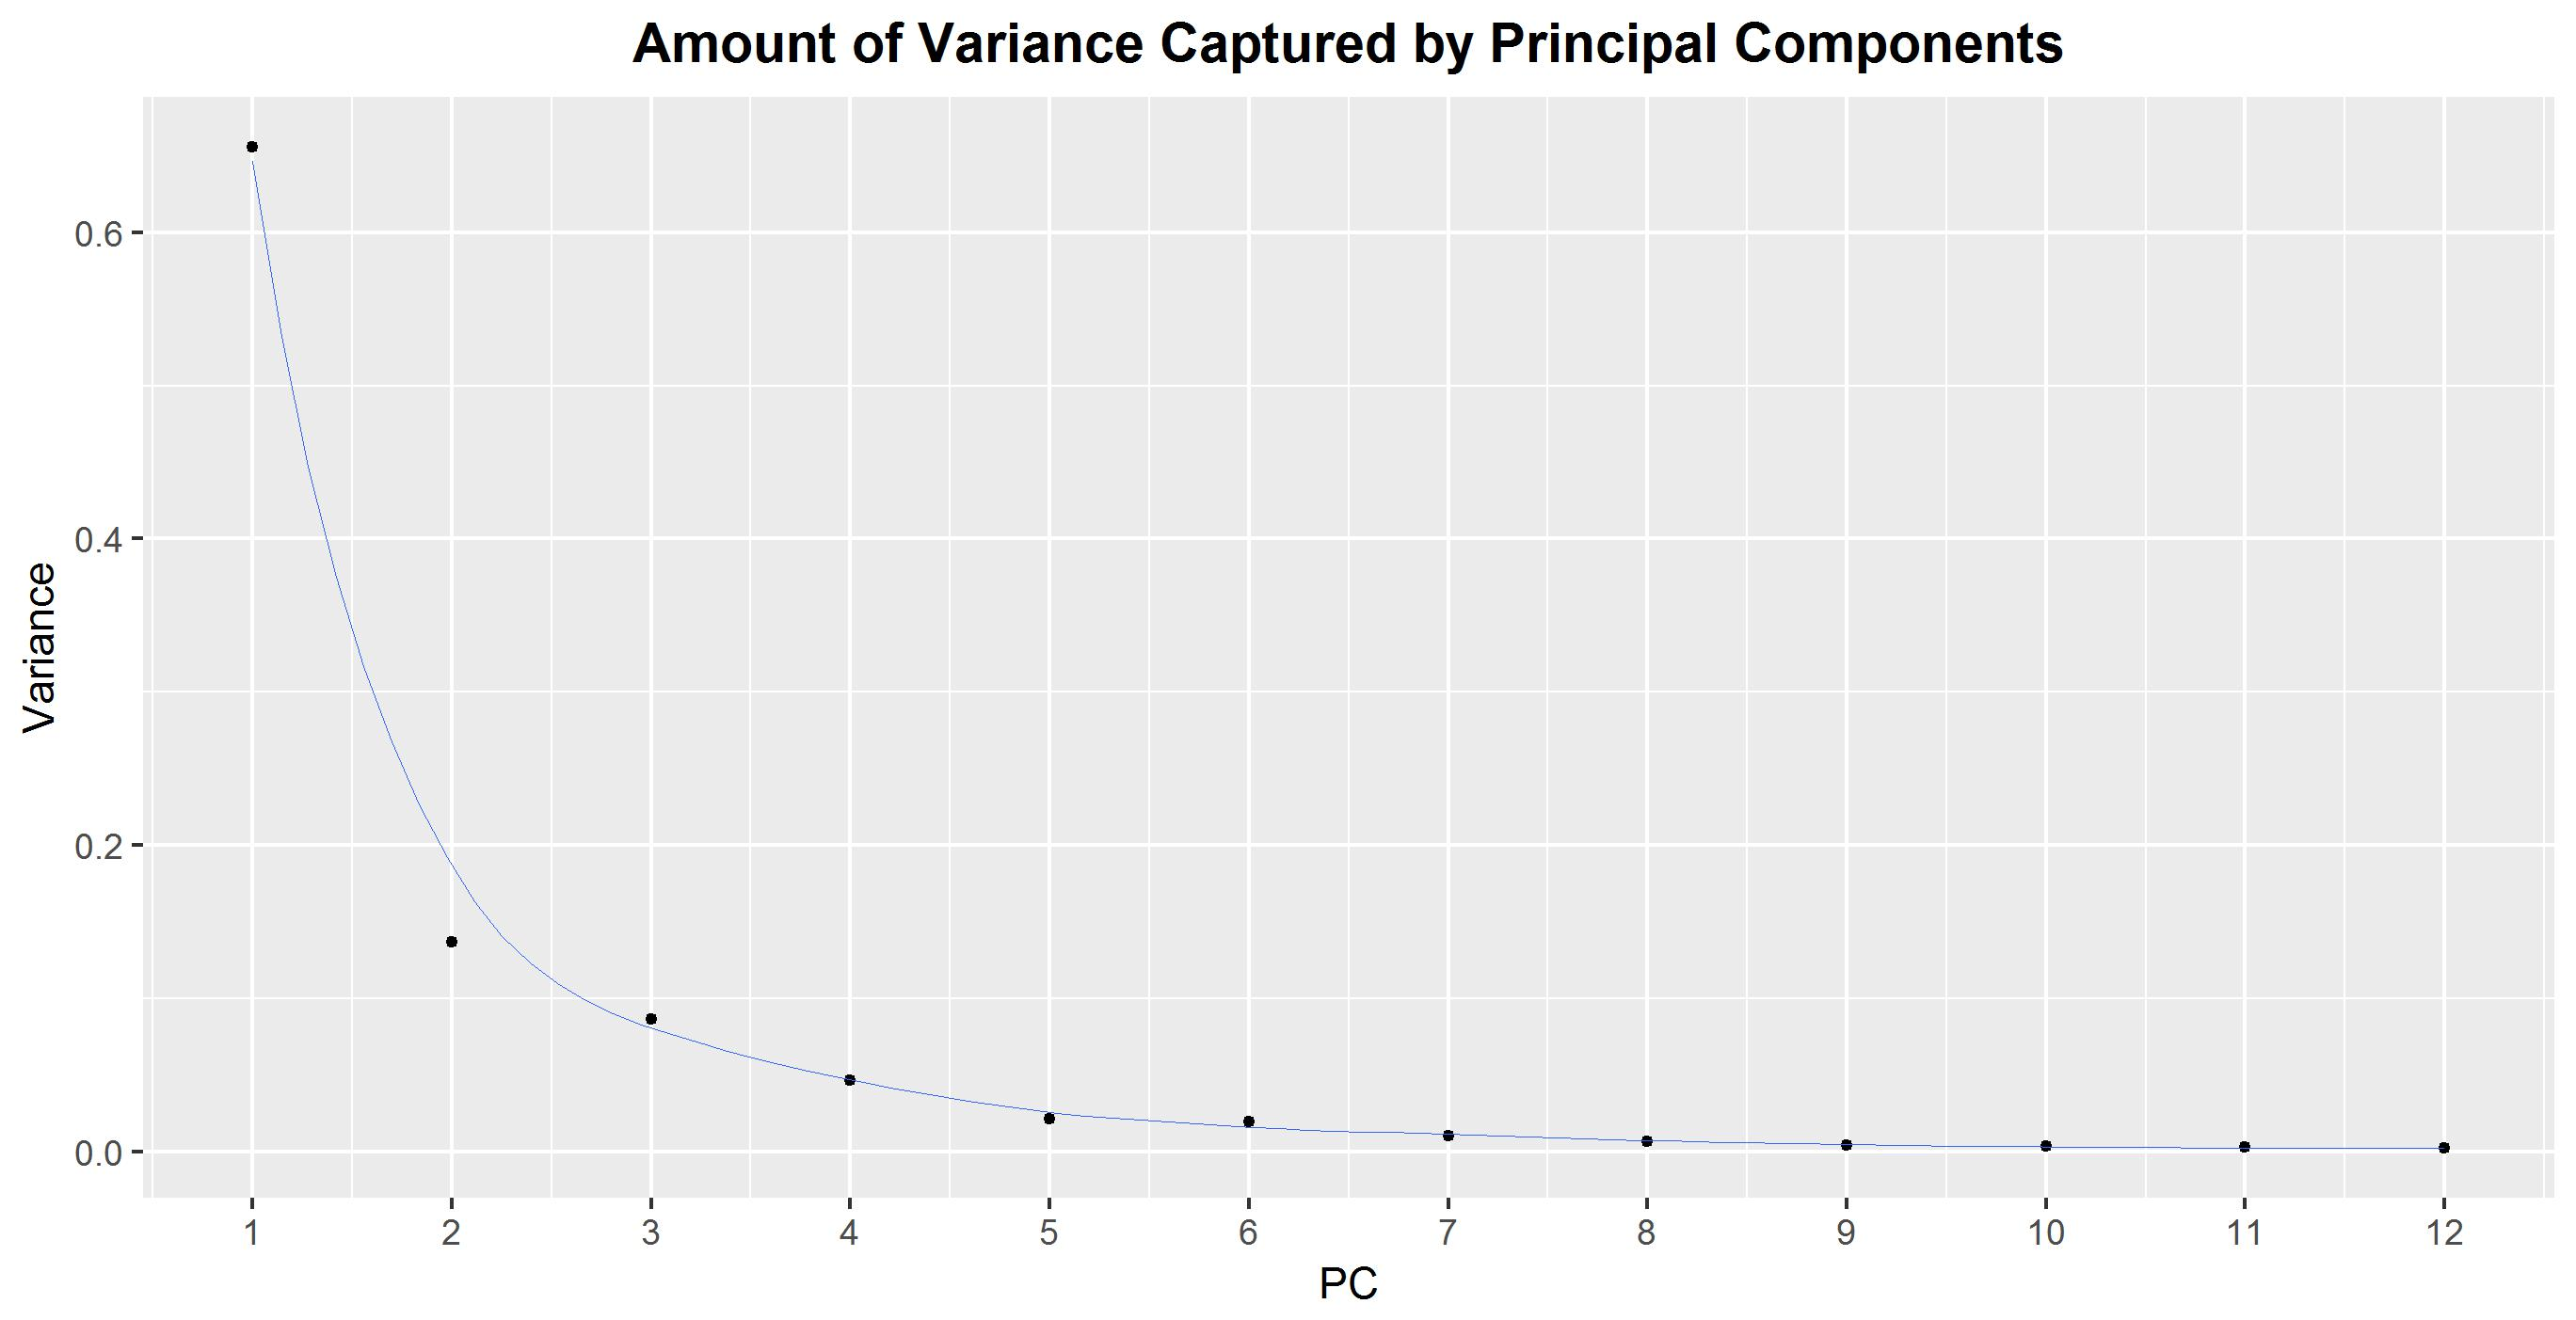
\includegraphics[width=\textwidth]{variancecapturedbypc.jpg}
\caption{\textbf{Variance Captured by First 12 Principal Components}}
\centering
\end{figure}

To carry out PCA, we used the preprocessing step SciPy to normalise all the input vectors to mean 0 and standard deviation 1. Subsequently, we perform principal components decomposition to obtain the eigenvector transformed representation of the dataset and their corresponding eigenvalues. We then fit 8 of the principal components that explained the largest amount of variance into the neural network to study if it can learn from the compressed representation of the input features. 
\subsubsection{Synthetic Minority Overrepresentation Technique (SMOTE)}
SMOTE is a statistical technique described in by Chawla et al. (2002) to overcome problems with imbalanced datasets that are common in machine learning. SMOTE oversamples the training class with fewer variables in a way that tries not to replicate data points (that makes certain data points over-represented) without creating new invalid training examples. It does this by taking the intersection of two nearest data points of the same training class. This can be seen in Figure 30. 

\begin{figure}[H]
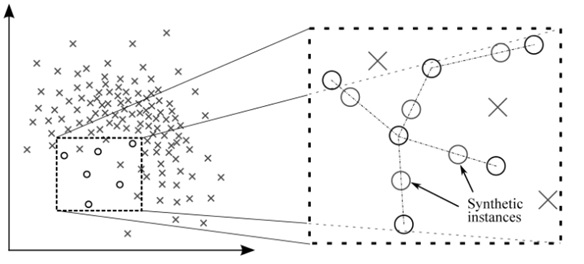
\includegraphics[width=\textwidth]{smoteoversampling.jpg}
\caption{\textbf{Illustration of SMOTE Oversampling Algorithm.} Note the use of 2 nearest neighbours to create a new synthetic example. Figure from Chawla et al., 2002}
\centering
\end{figure}

In doing so, it creates a more generalised representation of the sample class with less training examples, without replicating certain datapoints and without creating invalid data. This enables intelligent oversampling of the dataset to balance out the positive and negative feature classes. SMOTE has been shown to be valid for other datasets including sentence boundary detection (Liu et al., 2006) and data mining (Chawla, 2005).
\newpage
\section{Bibilography}

\begin{list}{}{%
\setlength{\topsep}{0pt}%
\setlength{\leftmargin}{0.5in}%
\setlength{\listparindent}{-0.5in}%
\setlength{\itemindent}{-0.5in}%
\setlength{\parsep}{\parskip}%
}%
\item[]\item[] Amagai, M. (2004). A mystery of AHNAK/desmoyokin still goes on. Journal of investigative dermatology 123, xiv.\\\item[] Abyzov, A., Li, S., Kim, D., Mohiyuddin, M., Stütz, A., Parrish, N., Mu, X., Clark, W., Chen, K., and Hurles, M. et al. (2015). Analysis of deletion breakpoints from 1,092 humans reveals details of mutation mechanisms. Nature Communications 6, 7256.\\\item[] Alizadeh, A., Eisen, M., Davis, E., Ma, C., Lossos, I., Rosenwald, A., Boldrick, J., Sabet, H., Tran, T., and Yu, X. (2017). Distinct types of diffuse large B-cell lymphoma identified by gene expression profiling. Nature 403, 503-511.\\\item[] Angrist, M. (2016). Personal genomics: Where are we now?. Applied \& translational genomics 8, 1.\\\item[] Anthimopoulos, M., Christodoulidis, S., Ebner, L., Christe, A., \& Mougiakakou, S. (2016). Lung pattern classification for interstitial lung diseases using a deep convolutional neural network. IEEE transactions on medical imaging 35, 1207-1216.\\\item[] Balkwill, F., \& Mantovani, A. (2001). Inflammation and cancer: back to Virchow?. The Lancet 357, 539-545.\\\item[] Bengio, Y., Simard, P., \& Frasconi, P. (1994). Learning long-term dependencies with gradient descent is difficult. IEEE transactions on neural networks 5, 157-166.\\\item[] Benjamini, Y., \& Speed, T. P. (2012). Summarizing and correcting the GC content bias in high-throughput sequencing. Nucleic acids research 40.\\\item[] Cantarel, B. L., Weaver, D., McNeill, N., Zhang, J., Mackey, A. J., \& Reese, J. (2014). BAYSIC: a Bayesian method for combining sets of genome variants with improved specificity and sensitivity. BMC bioinformatics 15, 104.\\\item[] Chawla, N. V. (2005). Data mining for imbalanced datasets: An overview. In Data mining and knowledge discovery handbook (pp. 853-867). Springer US.\\\item[] Chawla, N. V., Bowyer, K. W., Hall, L. O., \& Kegelmeyer, W. P. (2002). SMOTE: synthetic minority over-sampling technique. Journal of Artificial Intelligence Research 16, 321-357.\\\item[] Chen, Y., Lin, Z., Zhao, X., Wang, G., \& Gu, Y. (2014). Deep learning-based classification of hyperspectral data. IEEE Journal of Selected topics in applied earth observations and remote sensing 7, 2094-2107. \\\item[] CLC bio. (2011). Genomics Workbench User Manual 4.8. Finlandsgade 10-12 DK- 8200 Aarhus N, Denmark\\\item[] Cornish, A., and Guda, C. (2015). A Comparison of Variant Calling Pipelines Using Genome in a Bottle as a Reference. Biomed Research International 2015, 1-11.\\\item[] Danecek, P., Auton, A., Abecasis, G., Albers, C., Banks, E., DePristo, M., Handsaker, R., Lunter, G., Marth, G., and Sherry, S. et al. (2011). The variant call format and VCFtools. Bioinformatics 27, 2156-2158.\\\item[] DePristo, M., Banks, E., Poplin, R., Garimella, K., Maguire, J., Hartl, C., Philippakis, A., del Angel, G., Rivas, M., and Hanna, M. et al. (2011). A framework for variation discovery and genotyping using next-generation DNA sequencing data. Nature Genetics 43, 491-498.\\\item[] Di Tommaso, P., Chatzou, M., Baraja, P. P., \& Notredame, C. (2014). A novel tool for highly scalable computational pipelines.\\\item[] Egan, J. P. (1975). Signal detection theory and ROC analysis.\\\item[] Emara, M., Turner, A. R., \& Allalunis-Turner, J. (2014). Adult, embryonic and fetal hemoglobin are expressed in human glioblastoma cells. International Journal of Oncology 44, 514-520.\\\item[] Escalona, M., Rocha, S., \& Posada, D. (2016). A comparison of tools for the simulation of genomic next-generation sequencing data. Nature Reviews Genetics 17, 459-469.\\\item[] Fawcett, T. (2006). An introduction to ROC analysis. Pattern recognition letters 27, 861-874.\\\item[] Garrison, E., \& Marth, G. (2012). Haplotype-based variant detection from short-read sequencing. arXiv preprint arXiv:1207.3907.\\\item[] Gézsi, A., Bolgár, B., Marx, P., Sarkozy, P., Szalai, C., \& Antal, P. (2015). VariantMetaCaller: automated fusion of variant calling pipelines for quantitative, precision-based filtering. BMC genomics 16, 1.\\\item[] Griffith, M., Griffith, O., Coffman, A., Weible, J., McMichael, J., Spies, N., Koval, J., Das, I., Callaway, M., and Eldred, J. et al. (2013). DGIdb: mining the druggable genome. Nature Methods 10, 1209-1210.\\\item[] Huval, B., Wang, T., Tandon, S., Kiske, J., Song, W., Pazhayampallil, J., Andriluka, M., Rajpurkar, P., Migimatsu, T., and Cheng-Yue, R. et al. (2017). An Empirical Evaluation of Deep Learning on Highway Driving. Arvix 1504.01716.\\\item[] Hwang, S., Kim, E., Lee, I., \& Marcotte, E. M. (2015). Systematic comparison of variant calling pipelines using gold standard personal exome variants. Scientific reports 5, 17875.\\\item[] Janitz, M. (Ed.). (2011). Next-generation genome sequencing: towards personalized medicine. John Wiley \& Sons.\\\item[] Jensen, F. V. (1996). An introduction to Bayesian networks (Vol. 210). London: UCL press.\\\item[] Johnson, S., Abal, E., Ahern, K., \& Hamilton, G. (2014). From science to management: using Bayesian networks to learn about Lyngbya. Statistical Science 29, 36-41.\\\item[] Jolliffe, I. (2002). Principal component analysis. John Wiley \& Sons, Ltd.\\\item[] Karolchik, D., Barber, G., Casper, J., Clawson, H., Cline, M., Diekhans, M., Dreszer, T., Fujita, P., Guruvadoo, L., and Haeussler, M. et al. (2017). The UCSC Genome Browser database: 2014 update. Nucleic Acids Res 42, D764-D770.\\\item[] Kelly, M., Alvero, A., Chen, R., Silasi, D., Abrahams, V., Chan, S., Visintin, I., Rutherford, T., and Mor, G. (2006). TLR-4 Signaling Promotes Tumor Growth and Paclitaxel Chemoresistance in Ovarian Cancer. Cancer Research 66, 3859-3868.\\\item[] Kingma, D., \& Ba, J. (2014). Adam: A method for stochastic optimization. arXiv preprint arXiv:1412.6980.\\\item[] Knudson, A. G. (2001). Two genetic hits (more or less) to cancer. Nature Reviews Cancer 1, 157-162.\\\item[] Lam, H., Clark, M., Chen, R., Chen, R., Natsoulis, G., O'Huallachain, M., Dewey, F., Habegger, L., Ashley, E., and Gerstein, M. et al. (2012). Performance comparison of whole-genome sequencing platforms. Nature Biotechnology 30, 562-562.\\\item[] Lamont, R., Tan, W., Innes, A., Parboosingh, J., Schneidman-Duhovny, D., Rajkovic, A., Pappas, J., Altschwager, P., DeWard, S., and Fulton, A. et al. (2016). Expansion of phenotype and genotypic data in CRB2-related syndrome. European Journal Of Human Genetics 24, 1436-1444.\\\item[] Landrum, M. J., Lee, J. M., Riley, G. R., Jang, W., Rubinstein, W. S., Church, D. M., \& Maglott, D. R. (2014). ClinVar: public archive of relationships among sequence variation and human phenotype. Nucleic acids research 42, D980-D985.\\\item[] LeCun, Y., Bengio, Y., \& Hinton, G. (2015). Deep learning. Nature 521, 436-444.\\\item[] Lee, I., Sohn, M., Lim, H., Yoon, S., Oh, H., Shin, S., Shin, J., Oh, S., Kim, J., and Lee, D. et al. (2014). Ahnak functions as a tumor suppressor via modulation of TGFß/Smad signaling pathway. Oncogene 33, 4675-4684.\\\item[] Li, H., Handsaker, B., Wysoker, A., Fennell, T., Ruan, J., Homer, N., Marth, G., Abecasis, G., and Durbin, R. (2009). The Sequence Alignment/Map format and SAMtools. Bioinformatics 25, 2078-2079.\\\item[] Linderman, M., Brandt, T., Edelmann, L., Jabado, O., Kasai, Y., Kornreich, R., Mahajan, M., Shah, H., Kasarskis, A., and Schadt, E. (2014). Analytical validation of whole exome and whole genome sequencing for clinical applications. BMC Medical Genomics 7.\\\item[] Liu, X., Han, S., Wang, Z., Gelernter, J., \& Yang, B. Z. (2013). Variant callers for next-generation sequencing data: a comparison study. PloS one, 8(9), e75619.\\\item[] Liu, Y., Stolcke, A., Shriberg, E., \& Harper, M. (2005, June). Using conditional random fields for sentence boundary detection in speech. In Proceedings of the 43rd Annual Meeting on Association for Computational Linguistics (pp. 451-458). Association for Computational Linguistics.\\\item[] López, V., Fernández, A., García, S., Palade, V., \& Herrera, F. (2013). An insight into classification with imbalanced data: Empirical results and current trends on using data intrinsic characteristics. Information Sciences 250, 113-141.\\\item[] Lusci, A., Pollastri, G., \& Baldi, P. (2013). Deep architectures and deep learning in chemoinformatics: the prediction of aqueous solubility for drug-like molecules. Journal of chemical information and modeling 53, 1563.\\\item[] Maas, A. L., Hannun, A. Y., \& Ng, A. Y. (2013, June). Rectifier nonlinearities improve neural network acoustic models. In Proc. ICML (Vol. 30, No. 1).\\\item[] Marron, T. U., Joyce, E. Y., \& Cunningham-Rundles, C. (2012). Toll-like receptor function in primary B cell defects. Frontiers in bioscience (Elite edition), 4, 1853.\\\item[] McKenna, A., Hanna, M., Banks, E., Sivachenko, A., Cibulskis, K., Kernytsky, A., Garimella, K., Altshuler, D., Gabriel, S., and Daly, M. et al. (2010). The Genome Analysis Toolkit: A MapReduce framework for analyzing next-generation DNA sequencing data. Genome Research 20, 1297-1303.\\\item[] Meldrum, C., Doyle, M. A., \& Tothill, R. W. (2011). Next-generation sequencing for cancer diagnostics: a practical perspective. Clin Biochem Rev, 32(4), 177-195.\\\item[] Metzker, M. L. (2010). Sequencing technologies—the next generation. Nature reviews genetics 11, 31-46.\\\item[] Mohiyuddin, M., Mu, J., Li, J., Bani Asadi, N., Gerstein, M., Abyzov, A., Wong, W., and Lam, H. (2015). MetaSV: an accurate and integrative structural-variant caller for next generation sequencing. Bioinformatics 31, 2741-2744.\\\item[] Moreau, Y., \& Tranchevent, L. C. (2012). Computational tools for prioritizing candidate genes: boosting disease gene discovery. Nature Reviews Genetics 13, 523-536.\\\item[] Nielsen, R., Paul, J. S., Albrechtsen, A., \& Song, Y. S. (2011). Genotype and SNP calling from next-generation sequencing data. Nature Reviews Genetics, 12(6), 443-451.\\\item[] O'Rawe, J., Jiang, T., Sun, G., Wu, Y., Wang, W., Hu, J., Bodily, P., Tian, L., Hakonarson, H., and Johnson, W. et al. (2013). Low concordance of multiple variant-calling pipelines: practical implications for exome and genome sequencing. Genome Medicine 5, 28.\\\item[] Pearson, K. (1901). Principal components analysis. The London, Edinburgh and Dublin Philosophical Magazine and Journal 6, 566.\\\item[] Pedregosa, F., Varoquaux, G., Gramfort, A., Michel, V., Thirion, B., Grisel, O., Blondel, M., Weiss, R., Dubourg, V., and Vanderplas, J. et al. (2017). Scikit-learn: Machine learning in Python. Journal Of Machine Learning Research 12, 2825-2830.\\\item[] Pourret, O., Naïm, P., \& Marcot, B. (Eds.). (2008). Bayesian networks: a practical guide to applications (Vol. 73). John Wiley \& Sons.\\\item[] Quail, M., Smith, M., Coupland, P., Otto, T., Harris, S., Connor, T., Bertoni, A., Swerdlow, H., and Gu, Y. (2012). A tale of three next generation sequencing platforms: comparison of Ion torrent, pacific biosciences and illumina MiSeq sequencers. BMC Genomics 13, 341.\\\item[] Rehm, H. L. (2017). Evolving health care through personal genomics. Nature Reviews Genetics.\\\item[] Ruder, S. (2016). An overview of gradient descent optimization algorithms. arXiv preprint arXiv:1609.04747.\\\item[] Sandmann, S., de Graaf, A. O., Karimi, M., van der Reijden, B. A., Hellström-Lindberg, E., Jansen, J. H., \& Dugas, M. (2017). Evaluating Variant Calling Tools for Non-Matched Next-Generation Sequencing Data. Scientific Reports 7.\\\item[] Satterwhite, E., Sonoki, T., Willis, T., Harder, L., Nowak, R., Arriola, E., Liu, H., Price, H., Gesk, S., and Steinemann, D. et al. (2001). The BCL11 gene family: involvement of BCL11A in lymphoid malignancies. Blood 98, 3413-3420.\\\item[] Schirmer, M., D’Amore, R., Ijaz, U. Z., Hall, N., \& Quince, C. (2016). Illumina error profiles: resolving fine-scale variation in metagenomic sequencing data. BMC bioinformatics 17, 125.\\\item[] Schmidhuber, J. (2015). Deep learning in neural networks: An overview. Neural networks 61, 85-117.\\\item[] Schork, N. J., Murray, S. S., Frazer, K. A., \& Topol, E. J. (2009). Common vs. rare allele hypotheses for complex diseases. Current opinion in genetics \& development 19, 212-219.\\\item[] Shtivelman, E., Cohen, F. E., \& Bishop, J. M. (1992). A human gene (AHNAK) encoding an unusually large protein with a 1.2-microns polyionic rod structure. Proceedings of the National Academy of Sciences 89, 5472-5476.\\\item[] Silver, D., Huang, A., Maddison, C., Guez, A., Sifre, L., van den Driessche, G., Schrittwieser, J., Antonoglou, J., Panneershelvam, V., and Lanctot, M. et al. (2017). Mastering the game of Go with deep neural networks and tree search. Nature 529, 484-489.\\\item[] Slavotinek, A. M. (2016). The Family of Crumbs Genes and Human Disease. Molecular Syndromology 7, 274-281.\\\item[] Spencer, D., Abel, H., Lockwood, C., Payton, J., Szankasi, P., Kelley, T., Kulkarni, S., Pfeifer, J., and Duncavage, E. (2013). Detection of FLT3 Internal Tandem Duplication in Targeted, Short-Read-Length, Next-Generation Sequencing Data. The Journal Of Molecular Diagnostics 15, 81-93.\\\item[] Srivastava, N., Hinton, G. E., Krizhevsky, A., Sutskever, I., \& Salakhutdinov, R. (2014). Dropout: a simple way to prevent neural networks from overfitting. Journal of Machine Learning Research 15, 1929-1958.\\\item[] Su, C., Borsuk, M. E., Andrew, A., \& Karagas, M. (2014, May). Incorporating prior expert knowledge in learning Bayesian networks from genetic epidemiological data. In Computational Intelligence in Bioinformatics and Computational Biology, 2014 IEEE Conference on (pp. 1-5). IEEE.\\\item[] Sun, Y., Wang, X., \& Tang, X. (2014). Deep learning face representation from predicting 10,000 classes. In Proceedings of the IEEE Conference on Computer Vision and Pattern Recognition (pp. 1891-1898).\\\item[] Sutskever, I., Martens, J., Dahl, G. E., \& Hinton, G. E. (2013). On the importance of initialization and momentum in deep learning. ICML 28, 1139-1147.\\\item[] Talwalkar, A., Liptrap, J., Newcomb, J., Hartl, C., Terhorst, J., Curtis, K., Bresler, M., Song, Y., Jordan, M., and Patterson, D. (2014). SMASH: a benchmarking toolkit for human genome variant calling. Bioinformatics 30, 2787-2795.\\\item[] Tentler, J., Tan, A., Weekes, C., Jimeno, A., Leong, S., Pitts, T., Arcaroli, J., Messersmith, W., and Eckhardt, S. (2012). Patient-derived tumour xenografts as models for oncology drug development. Nature Reviews Clinical Oncology 9, 338-350.\\\item[] Tieleman, T. and Hinton, G. Lecture 6.5 - RMSProp, COURSERA: Neural Networks for Machine Learning. Technical report, 2012\\\item[] Tsiatis, A. C., Norris-Kirby, A., Rich, R. G., Hafez, M. J., Gocke, C. D., Eshleman, J. R., \& Murphy, K. M. (2010). Comparison of Sanger sequencing, pyrosequencing, and melting curve analysis for the detection of KRAS mutations: diagnostic and clinical implications. The Journal of Molecular Diagnostics 12, 425-432.\\\item[] Van Der Maaten, L., Postma, E., \& Van den Herik, J. (2009). Dimensionality reduction: a comparative. J Mach Learn Res, 10, 66-71.\\\item[] Van Rossum, G. (2007, June). Python Programming Language. In USENIX Annual Technical Conference (Vol. 41, p. 36).\\\item[] Wang, K., Li, M., \& Hakonarson, H. (2010). ANNOVAR: functional annotation of genetic variants from high-throughput sequencing data. Nucleic acids research 38, e164-e164.\\\item[] Wei, Z., Wang, W., Hu, P., Lyon, G. J., \& Hakonarson, H. (2011). SNVer: a statistical tool for variant calling in analysis of pooled or individual next-generation sequencing data. Nucleic acids research 39, e132-e132.\\\item[] Weniger, M., Pulford, K., Gesk, S., Ehrlich, S., Banham, A., Lyne, L., Martin-Subero, J., Siebert, R., Dyer, M., and Möller, P. et al. (2006). Gains of the proto-oncogene BCL11A and nuclear accumulation of BCL11AXL protein are frequent in primary mediastinal B-cell lymphoma. Leukemia 20, 1880-1882.\\\item[] Windecker, S., Stortecky, S., Stefanini, G., da Costa, B., Rutjes, A., Di Nisio, M., Silletta, M., Maione, A., Alfonso, F., and Clemmensen, P. et al. (2014). Revascularisation versus medical treatment in patients with stable coronary artery disease: network meta-analysis. BMJ 348.\\\item[] Xie, M., Lu, C., Wang, J., McLellan, M., Johnson, K., Wendl, M., McMichael, J., Schmidt, H., Yellapantula, V., and Miller, C. et al. (2014). Age-related mutations associated with clonal hematopoietic expansion and malignancies. Nature Medicine 20, 1472-1478.\\\item[] Yan, Y., Chen, M., Shyu, M. L., \& Chen, S. C. (2015, December). Deep learning for imbalanced multimedia data classification. In Multimedia (ISM), 2015 IEEE International Symposium on (pp. 483-488).\\\item[] Ye, K., Schulz, M. H., Long, Q., Apweiler, R., \& Ning, Z. (2009). Pindel: a pattern growth approach to detect break points of large deletions and medium sized insertions from paired-end short reads. Bioinformatics 25, 2865-2871.\\\item[] Zeiler, M. D. (2012). ADADELTA: an adaptive learning rate method. arXiv preprint arXiv:1212.5701.\\\item[] Zhang, H., Gao, J., Zhao, Z., Li, M., \& Liu, C. (2014). Clinical implications of SPRR1A expression in diffuse large B-cell lymphomas: a prospective, observational study. BMC cancer 14, 333.\\\item[] Zook, J. M., Chapman, B., Wang, J., Mittelman, D., Hofmann, O., Hide, W., \& Salit, M. (2014). Integrating human sequence data sets provides a resource of benchmark SNP and indel genotype calls. Nature biotechnology 32, 246-251.\\


\end{list}

\newgeometry{a4paper,bindingoffset=0.2in, margin=1in}
\newpage
\section{Relevant Code}
3 code segments are provided to clarify the implementation of generating the matrixes for deep learning, deep learning networks and finally bayesian networks. Other code segments not shown include the code base for parsing vcf input into features, concordance generators, NextFlow and Bash code used to simulate and process genomic data as well as to control deep learning and analytic pipelines, and other python helper scripts (e.g. comparing two VCF files, analysis with pre-trained network).
\subsection{generate\_matrixes.py}
\begin{minted}[linenos=true,numberblanklines=true,showspaces=false,breaklines=true,
fontsize=\footnotesize,breakautoindent=true]{python}
#This python script generates the set of matrixes to be used in deep learning, and then calls the main method that trains the deep learning network.
#Input : a directory that contains all the vcf files for processing, as well as a truth file. 
#Output : np.arrays of features from generate_matrixes with accompanying truth labels, feature set lengths, a dictionary of vcf object records, as well as the list of relevant sample features for easy reference
#Notes :
#Vcf files should have the "vcf" string in their name and truth file should have a "truth" string in its name.
#No other file should be present in the folder
#Overall Strategy :
#Generate a dictionary of lists, where the keys are mutations, and the value is contains a matrix containing information of all five callers
#Secondly, for each mutation label, check if it is inside the truth file or not. The truth is preloaded into a dictionary
#Finally, pass the set of features with accompanying truth labels to the neural network 
#The main datastructure used are python dictionaries, which allows O(1) dictionary lookup times 

import os  
import time
from ANNgenerateresults import *  #this file contains all the main methods for actual neural network training
from methods import *  #this file contains all the methods for parsing each VCF entry into a numerical list of features

#declare names of useful files that contains processed data to be saved
LIST_OF_INPUTS_NAME = '/ANN/samplelist.p'     
TRUTH_DICTIONARY_NAME = '/ANN/truthdict.p'
CALLER_LENGTH_FILE_NAME = '/ANN/callerlengths.txt'
VCF_LIST_FILE_NAME = '/ANN/vcf_list.p'
SCORES_NAME = '/ANN/scores.txt'
Y_DATA_NAME = '/ANN/myydata.txt'
X_DATA_NAME = '/ANN/myXdata.txt'

#Initialise NUMBER_OF_CALLERS
NUMBER_OF_CALLERS = 5


# This method follows the typical input output processing pipeline 
# It takes in the user input, and loads it into local variables. 
# It then executes another method, main_analyse_samples_and_truth on the loaded variables
# Finally, it then saves files into a directory determined by the final variables, and calls the next step of the pipeline
# the neural network training, which is main_gather_input_execute_prep_output

def load_and_save_data(user_input):
    user_input = vars(user_input)   
    input_samples, referencepath, output_location = load_references(user_input)   # load user input
    my_x_dataset, my_y_dataset, list_of_samples, truth_dictionary, length_of_caller_outputs, \
    vcf_record_list = main_analyse_samples_and_truth(input_samples, referencepath) 
    save_files(output_location, my_x_dataset, length_of_caller_outputs,
               list_of_samples, truth_dictionary, vcf_record_list, my_y_dataset) 
    orig_stdout = sys.stdout  #save print statements into stdout
    f = file(str(output_location) + SCORES_NAME, 'w')
    sys.stdout = f
    main_gather_input_execute_prep_output(length_of_caller_outputs, truth_dictionary, my_x_dataset, my_y_dataset, list_of_samples, output_location, vcf_record_list) 

# This method first prepares a dictionary of truth to be checked against. It then initialises
# a dictionary of samples with all the keys, each key being a variant call, and then fills it up each key with data from each caller
# subsequently, it removes dictionary entries that are the wrong size, and then checks whether
# each entry in the dictionary is true or not by looking up the truth dictionary
# subsequently it performs array balancing, and converts the data to np.array, as well as the dictionary of truth
# and list of called samples

def main_analyse_samples_and_truth(path, referencepath):
    os.chdir(path)
    truthdict = generate_truth_list(path)       
    print "truth dictionary generated at time :", time.time() - start
    callerlengths, list_of_called_samples, vcf_list = generate_input(path, referencepath)
    print "samples generated at time :", time.time() - start
    clean_truth_array, cleaned_sample_array = check_predicted_with_truth(list_of_called_samples, truthdict)
    print "samples checked with truth at time :", time.time() - start
    cleaned_sample_array = np.array(cleaned_sample_array, np.float64)
    clean_truth_array = np.array(clean_truth_array)
    return cleaned_sample_array, clean_truth_array, list_of_called_samples, truthdict, callerlengths, vcf_list

# This method generates the truth dictionary, by iterating through the vcf file, parsing all the vcf entries and appending them all as keys in the dictionary 

def create_truth_dictionary(generated_truth_dictionary, truth_file):
    vcf_reader = vcf.Reader(open(truth_file, 'r'))    
    for record in vcf_reader:
        if "GL" in record.CHROM:    #Ignore non-regular chromosomes in our dataset
            continue
        templist = []
        for item in record.ALT:
            templist.append(str(item).upper())          #Alternates might be a list, so they have to be saved as a immutable tuple
        generated_truth_dictionary[(str(record.CHROM), str(record.POS), str(record.REF).upper())] = tuple(templist)

# This method generates the input dictionary, by first initialising the keys of the dictionary by iterating through the vcf file once, and then
# Iterating through the vcf file again and parsing all the entries as input vectors

def generate_input(path, referencepath):
    reference_dictionary = get_reference_dictionary_for_entropy(referencepath)
    base_entropy = get_ref_entropy(referencepath)
    full_dictionary = get_dictionary_keys(path)
    list_of_called_samples, callerlengths, vcf_list = fill_sample_dictionary(base_entropy, full_dictionary, path, reference_dictionary)
    return callerlengths, list_of_called_samples, vcf_list


# This method goes through all the training variant calling files and extracts unique calls as keys in the sample dictionary

def get_dictionary_keys(path):
    sample_dictionary = {}
    for vcf_file in os.listdir(path):
        if ignore_file(vcf_file):
            continue
        vcf_reader = vcf.Reader(open(vcf_file, 'r'))
        sample_dictionary = create_dictionary_keys(vcf_reader, sample_dictionary)
    return sample_dictionary

#This method ensures the feature vector is in the right order - the entries must always be in the order fb, hc, ug, pindel and st.

def create_list_of_paths(path):
    list_of_paths = [0] * NUMBER_OF_CALLERS
    for vcf_file in os.listdir(path):
        if ignore_file(vcf_file):
            continue
        if "fb" in vcf_file:
            list_of_paths[0] = vcf_file
        if "hc" in vcf_file:
            list_of_paths[1] = vcf_file
        if "ug" in vcf_file:
            list_of_paths[2] = vcf_file
        if "pind" in vcf_file:
            list_of_paths[3] = vcf_file
        if "st" in vcf_file:
            list_of_paths[4] = vcf_file
    return list_of_paths

# This method goes through all the training variant calling files and fills each entry in a sample dictionary
# with data. If it is empty, it returns an array of length n, where n is the number of variables
# that same caller would have provided.
# Each caller has a different amount of variables because it contains different datasets

def fill_sample_dictionary(base_entropy, sample_dictionary, path, reference_dictionary):
    callerlengths = [0] * number_of_callers
    index = 0
    total_mode_value = 0
    list_of_paths = create_list_of_paths(path)
    for vcf_file in list_of_paths:
        index += 1
        opened_vcf_file = vcf.Reader(open(vcf_file, 'r'))
        removaldict = iterate_over_file_to_extract_data(base_entropy, sample_dictionary,
                                                        reference_dictionary, opened_vcf_file, vcf_file)
        mode_value = get_mode_value(removaldict)
        add_length_to_caller_lengths_based_on_file_name(vcf_file, mode_value, callerlengths)
        refill_dictionary_with_zero_arrays_for_each_file(sample_dictionary, index, mode_value)
        total_mode_value += mode_value
    list_of_passed_samples, vcf_list = add_mode_values_into_list_of_samples(sample_dictionary, total_mode_value)
    return list_of_passed_samples, callerlengths, vcf_list


# this method fills the dictionary with empty arrays with the same length as the ones that were supposed to be added

def refill_dictionary_with_zero_arrays_for_each_file(full_dictionary, index, length_of_data_array):
    empty_set = []
    for i in range(length_of_data_array):
        empty_set.append(0)
    for item in full_dictionary:
        checksum = len(full_dictionary[item][0])
        if checksum < index:
            arbinfo = empty_set
            full_dictionary[item][0].append(arbinfo)


# this method iterates through all the files to extract data from each sample. It uses methods from the
# methods.py function, which parses each record for data.

def iterate_over_file_to_extract_data(base_entropy, sample_dictionary, recorddictionary, vcf_reader1, vcf_file):
    removaldict = {}
    for record in vcf_reader1:
        if "GL" in str(record.CHROM):
            continue
        sample_name = get_sample_name_from_record(record)
        sample_data = getallvalues(record, recorddictionary, base_entropy, vcf_file)
        sample_dictionary[sample_name][0].append(sample_data)
        sample_dictionary[sample_name][1] = record
        create_removal_dict(sample_data, removaldict)
    return removaldict

# this method counts the mode number of entries in the dictionary. Due to certain vcf files having multiple possible number of entries for a field, this will create an error
# as the size of the input arrays should always be constant. Thus, any sample that does not fit the array should be removed. 
# TO-DO See if a better implementation can be done that doesn't reduce data available
	
def create_removal_dict(sample_data, removaldict):
    count = 0
    count += len(sample_data)
    if count not in removaldict:
        removaldict[count] = 1
    else:
        removaldict[count] += 1


# this method prepares the reference genome dictionary for use in entropy calculations

def get_reference_dictionary_for_entropy(reference_path):
    record_dictionary = SeqIO.to_dict(SeqIO.parse(reference_path, "fasta"), key_function=get_chr)
    return record_dictionary

# this method ensures that the files inputed are correct

def ignore_file(vcf_file):
    if "vcf" not in vcf_file or "truth" in vcf_file:
        return True
    return False

# this method creates the set of keys for the dictionary
	
def create_dictionary_keys(vcf_reader, sample_dictionary):
    for record in vcf_reader:
        if "GL" in str(record.CHROM):
            continue
        sample_name = get_sample_name_from_record(record)
        sample_dictionary[sample_name] = [[], []]  # fullname has become a key in fulldictionary
    return sample_dictionary

# standard method that returns a tuple of the variant call object with the chromosome, position, reference and tuple of alternates

def get_sample_name_from_record(record):
    templist = []
    for item in record.ALT:
        templist.append(str(item).upper())
    sample_name = (str(record.CHROM), str(record.POS), str(record.REF).upper(), tuple(templist))
    return sample_name

# this method sets the length of the input neural networks
	
def add_length_to_caller_lengths_based_on_file_name(vcf_file, caller_length, callerlengths):
    if "fb" in vcf_file:
        callerlengths[0] = caller_length
    if "hc" in vcf_file:
        callerlengths[1] = caller_length
    if "ug" in vcf_file:
        callerlengths[2] = caller_length
    if "pind" in vcf_file:
        callerlengths[3] = caller_length
    if "st" in vcf_file:
        callerlengths[4] = caller_length

# this method wraps the create truth dictionary method and is used to checking that the dictionary file has the correct name
		
def generate_truth_list(path):
    generated_truth_dictionary = {}
    for truth_file in os.listdir(path):
        if "truth" not in truth_file:
            continue
        create_truth_dictionary(generated_truth_dictionary, truth_file)
    return generated_truth_dictionary

# this method takes in the mutation (in a tuple) and checks if that mutation exists in the truth dictionary
# A mutation exists if the chromosome, reference and position of the variant call is correct, AND one of the alternate alleles it contains
# is also an alternate allele in the truth dataset
	
def check_sample_against_truth_dictionary(tuple_name, final_truth_list, truth_dictionary):
    temp_tuple = (tuple_name[0], tuple_name[1], tuple_name[2])
    if temp_tuple in truth_dictionary:
        for alternate in tuple_name[3]:
            if alternate in truth_dictionary[temp_tuple]:
                final_truth_list.append(1)
                return
    final_truth_list.append(0)
    return

# This method loads the paths of the files into local variables

def load_references(user_input):
    file1 = user_input['input'][0]
    referencepath = user_input['reference']
    output_location = user_input['output']
    return file1, referencepath, output_location

# This method saves all the processed data into files that can be used for other purposes later or loaded natively instead of doing the processing again

def save_files(output_location, x_array, length_of_caller_outputs, sample_list, truth_dict, vcf_dictionary_file,
               y_array=[]):
    file2 = output_location
    x_data_file_name = str(file2) + str(X_DATA_NAME)
    np.save(x_data_file_name, x_array)
    vcf_file_name = str(file2) + str(VCF_LIST_FILE_NAME)
    caller_length_file_name = str(file2) + str(CALLER_LENGTH_FILE_NAME)
    truth_dictionary_name = str(file2) + str(TRUTH_DICTIONARY_NAME)
    list_of_inputs_name = str(file2) + str(LIST_OF_INPUTS_NAME)
    np.save(caller_length_file_name, length_of_caller_outputs)
    with open(list_of_inputs_name, 'wb') as samplesave1:
        pickle.dump(sample_list, samplesave1)
    with open(truth_dictionary_name, 'wb') as samplesave2:
        pickle.dump(truth_dict, samplesave2)
    with open(vcf_file_name, 'wb') as samplesave3:
        pickle.dump(vcf_dictionary_file, samplesave3)
    if y_array != []:
        y_data_file_name = str(file2) + str(Y_DATA_NAME)
        np.save(y_data_file_name, y_array)

# This method takes in two dictionaries, a dictionary of truth mutations and a dictionary of sample mutations, 
# checks whether each of the sample variables are inside the truth dictionary
# and returns 2 arrays, an array of samples and an array of accompanying truth labels
		
def check_predicted_with_truth(passed_list_of_samples, dictionary_of_truth=[]):
    final_array_of_samples = []
    final_truth_list = []
    for item in passed_list_of_samples:
        if dictionary_of_truth:
            check_sample_against_truth_dictionary(item[0], final_truth_list, dictionary_of_truth)
        temp_array = []
        for row in item[1]:
            temp_array.extend(row)
        final_array_of_samples.append(temp_array)
    if dictionary_of_truth:
        return final_truth_list, final_array_of_samples
    return final_array_of_samples

# This method ensures that only the variables that have the modal number of features are used 
# in neural network training to ensure all array sizes are the same

def add_mode_values_into_list_of_samples(full_dictionary, mode_value):
    list_of_passed_samples = []
    vcf_list = []
    for key in full_dictionary:
        second_count = 0
        for item in full_dictionary[key][0]:
            second_count += len(item)
        if second_count != mode_value:
            continue
        list_of_passed_samples.append([key, full_dictionary[key][0]])
        vcf_list.append(full_dictionary[key][1])
    return list_of_passed_samples, vcf_list

# This method gets the modal number of features from a modal dictionary

def get_mode_value(removaldict):
    curr = 0
    mode_value = 0
    for new_key in removaldict:
        if removaldict[new_key] > curr:
            curr = removaldict[new_key]
            mode_value = new_key
    return mode_value

# This method iterates through the dataset to create a modal dictionary which contains a key-value pair of (number of features - number of times seen).
# The mode number of features is kept
	
def iterate_through_dictionary_to_find_mode_size(full_dictionary):
    removaldict = {}
    samples = 0
    for key in full_dictionary:
        samples += 1
        if samples == sample_limit:
            break
        count = 0
        for item in full_dictionary[key]:
            count += len(item)
        if count not in removaldict:
            removaldict[count] = 1
        else:
            removaldict[count] += 1
    return removaldict


if __name__ == "__main__":
    np.seterr(divide='raise', invalid='raise')
    parser = argparse.ArgumentParser(description="train neural net")
    parser.add_argument('-i', '--input', help="give directories with files", nargs='+')
    parser.add_argument('-d', '--debug', help="look at matrixes built")
    parser.add_argument('-r', '--reference', help="")
    parser.add_argument('-o', '--output', help="")
    paths = parser.parse_args()
    start = time.time()
    load_and_save_data(paths)                              
\end{minted}
\subsection{train\_network.py}

\begin{minted}[linenos=true,numberblanklines=true,showspaces=false,breaklines=true,
fontsize=\footnotesize,breakautoindent=true]{python}
#This script is called by the generate_matrixes.py script and contains the implementation of the neural network.
#Input : np.arrays of features from generate_matrixes with accompanying truth labels, feature set lengths, a dictionary of vcf object records, as well as the list of sample features 
#Output : A VCF file containing all the filtered entries by the neural network, as well the list of accompanying scores 
#Overall Strategy :
#Perform SMOTE oversampling of the input features, and then use the features to train the neural network
#After training, perform validation on test dataset, and subsequently prepare a vcf file with filtered entries


#import all necessary components 
import argparse
import cPickle as pickle
import sys
import numpy as np
import vcf
from imblearn.over_sampling import SMOTE
from keras.callbacks import *
from keras.layers import Dense, Dropout, Activation
from keras.layers.advanced_activations import LeakyReLU
from keras.layers.normalization import BatchNormalization
from keras.models import Sequential
from keras.models import load_model
from keras.optimizers import RMSprop
from sklearn.metrics import *
from sklearn.model_selection import train_test_split


#set constants
PCA_COMPONENTS = 8
STEP_INCREMENT = 10
RECURSION_LIMIT = 0.0002
VERBOSE = 1
seed = 1337

# Initialise random seed for reproducibility
np.random.seed(seed) 

#Prepare file names for saving
vcf_file_name = "/ANN/truevcf.vcf"
keras_model_name = "/ANN/model"
model_truth_name = "/ANN/modeltruths.txt"
model_predictions_name = "/ANN/modelpredictions.txt"
original_vcf_reader = "/data/backup/metacaller/stage/data/version6.3a/hc.vcf.normalisedtrain.vcf"

# this method takes in a path and returns training matrixes for the ANN
# The path should contain n caller vcf files and 1 truth file
# vcf files should be labelled with vcf and truth file should be labelled with truth
# no other file should be present in the folder
def main_gather_input_execute_prep_output(array_sizes, dict_of_truth_input, fullmatrix_sample, fullmatrix_truth, list_of_samples_input, save_location, vcf_dictionary):
    calculated_prediction_actual, calculated_truth_actual = train_neural_net(20, 10, fullmatrix_sample, fullmatrix_truth,                                                                             save_location, array_sizes)
    get_all_relevant_scores(calculated_prediction_actual, calculated_truth_actual, dict_of_truth_input, list_of_samples_input, vcf_dictionary, save_location)

# This method counts the number of false negatives inside the input sample

def count_false_negative(calculated_prediction_actual, calculated_truth_actual):
    count_false_negative = 0
    for i in range(len(calculated_prediction_actual)):
        if calculated_prediction_actual[i] == 0 and calculated_truth_actual[i] == 1:
            count_false_negative += 1
    return count_false_negative

# this is the wrapper function for the recursive hill climbing algorithm to get the best f1 score
# It starts from a low threshold value, and marginally increases the threshold until it is unable to find
# any better F1 scores. It then reports the threshold, F1 score and produces the filtered callset 

def get_all_relevant_scores(calculated_prediction_actual, calculated_truth_actual, dict_of_truth_input,
                            list_of_samples_input, vcf_list, outputpath):
    print "Here are some predictions", calculated_prediction_actual[:100]
    print "here are some truths", calculated_prediction_actual[:100]
    f1_score_left = get_scores(calculated_prediction_actual, calculated_truth_actual, 0.0, list_of_samples_input, dict_of_truth_input)
    guess_f1_final_score, guess_f1_final = recursive_best_f1_score(calculated_prediction_actual,   calculated_truth_actual, dict_of_truth_input, list_of_samples_input, 0.0, f1_score_left, 0.2)
    get_scores(calculated_prediction_actual, calculated_truth_actual, guess_f1_final, list_of_samples_input, dict_of_truth_input, VERBOSE)
    produce_vcf_file(calculated_prediction_actual, guess_f1_final, list_of_samples_input, vcf_list, outputpath)

# This method produces the vcf file through filtering with the neural network threshold calls

def produce_vcf_file(calculated_prediction_actual, guess_f1_final, list_of_samples_input, vcf_list, outputpath):
    prediction = []
    for item in calculated_prediction_actual:
        if item > guess_f1_final:
            prediction.append(1)
        else:
            prediction.append(0)
    list_of_records = []
    for i in range(len(list_of_samples_input)):
        if prediction[i] == 1:
            list_of_records.append(vcf_list[i])
    vcf_reader = vcf.Reader(filename=original_vcf_reader)
    vcf_writer = vcf.Writer(open(outputpath + vcf_file_name, 'w'), vcf_reader)
    for record in list_of_records:
        vcf_writer.write_record(record)

# This method is the recursive function that attempts to find the threshold that produces the best f1 score. It does this
# by iterating through steps of thresholds (0.2, 0.02 and 0.002) until no better F1 score can be found for a marginal increase in threshold. 
# It then returns the best F1 score and the threshold

def recursive_best_f1_score(calculated_prediction_actual, calculated_truth_actual, dict_of_truth_input,
                            list_of_samples_input, guess, guess_score, step):
    if step <= RECURSION_LIMIT:
        return guess_score, guess
    new_guess = guess + step
    new_guess_score = get_scores(calculated_prediction_actual, calculated_truth_actual, new_guess,
                                 list_of_samples_input, dict_of_truth_input)
    if new_guess_score > guess_score:
        return recursive_best_f1_score(calculated_prediction_actual, calculated_truth_actual, dict_of_truth_input,
                                       list_of_samples_input, new_guess, new_guess_score, step)
    return recursive_best_f1_score(calculated_prediction_actual, calculated_truth_actual, dict_of_truth_input,
                                   list_of_samples_input, guess, guess_score, step / STEP_INCREMENT)

# this method uses pre-loaded data to train the neural network. It is optional and only used when this python script is called natively and not imported

def load_references(input_paths):
    input_paths = vars(input_paths)
    fullmatrix_sample = np.load(input_paths['input'][0])
    fullmatrix_truth = np.load(input_paths['input'][1])
    with open(input_paths['input'][3], 'rb') as fp1:
        list_of_samples_input = pickle.load(fp1)
    with open(input_paths['input'][4], 'rb') as fp2:
        dict_of_truth_input = pickle.load(fp2)
    array_sizes = np.load(input_paths['input'][5])
    with open(input_paths['input'][6], 'rb') as fp3:
        vcf_dictionary = pickle.load(fp3)
    orig_stdout = sys.stdout
    f = file(str(input_paths['input'][3]) + '.txt', 'w')
    sys.stdout = f
    return array_sizes, dict_of_truth_input, fullmatrix_sample, fullmatrix_truth, list_of_samples_input, input_paths, vcf_dictionary

# this method solves the double false negative problem that is created due to the neural network prediction scheme
	
def remove_duplicated_false_negative(prediction_list, truth_list, false_negatives):
    count = 0
    removal_list = []
    for i in range(len(prediction_list) - 1, -1, -1):
        if count == false_negatives:
            break
        if prediction_list[i] == 0 and truth_list[i] == 1:
            removal_list.insert(0, i)
            count += 1
    for index in removal_list:
        prediction_list.pop(index)
        truth_list.pop(index)
    return prediction_list, truth_list

# this method takes in the binary truth and predicted samples and calculates the true positive rate, false positive rate, recall, precision and f1 score
	
def get_scores(actual_predictions, actual_truth, value, sample_list, truth_dictionary, verbose=0):
    temp_actual_truth = list(actual_truth)
    prediction = []
    for item in actual_predictions:
        if item > value:
            prediction.append(1)
        else:
            prediction.append(0)
    false_negatives = count_false_negative(actual_predictions, actual_truth)
    finalpredictionnumbers, finaltruthnumbers = add_negative_data(sample_list, truth_dictionary, prediction, temp_actual_truth)
    finalpredictionnumbers, finaltruthnumbers = remove_duplicated_false_negative(finalpredictionnumbers, finaltruthnumbers, false_negatives)
    final_f1_score = f1_score(finaltruthnumbers, finalpredictionnumbers)
    if verbose:
        print_scores(actual_truth, final_f1_score, finalpredictionnumbers, finaltruthnumbers, prediction, value)
    return final_f1_score

# default method for printing all relevant scores
	
def print_scores(actual_truth, final_f1_score, finalpredictionnumbers, finaltruthnumbers, prediction, value):
    final_false_positive, final_true_negative = perf_measure(finaltruthnumbers, finalpredictionnumbers)
    print "final false positive rate is :", final_false_positive
    print "final true negative rate is :", final_true_negative
    print "final precision score is :", precision_score(finaltruthnumbers, finalpredictionnumbers)
    print "final recall score is :", recall_score(finaltruthnumbers, finalpredictionnumbers)
    print "threshold is", value
    print "final F1 score is : ", final_f1_score

# This method looks at the set of predicted samples and the set of truths and adds the false negatives to the predicted sample.
	
def add_negative_data(list_of_samples, dict_of_truth, array_of_predicted, array_of_truth):
    dict_of_samples = generate_sample_dictionary(array_of_predicted, list_of_samples)
    list_of_truth = generate_list_of_truth(dict_of_truth)
    new_array_of_predicted = list(array_of_predicted)
    new_array_of_truth = list(array_of_truth)
    original_length = len(new_array_of_predicted)
    for item in list_of_truth:
        fillnegative(item, dict_of_samples, new_array_of_predicted, new_array_of_truth)
    print "number of false data samples are", (len(new_array_of_predicted) - original_length)
    return new_array_of_predicted, new_array_of_truth

# This method generates a list of truth variant calls from a dictionary of truth variant calls.

def generate_list_of_truth(dict_of_truth):
    list_of_truth = []
    for key in dict_of_truth:
        mytuple = dict_of_truth[key]
        temptuple = []
        for item in mytuple:
            temptuple.append(item)
        list_of_truth.append([key[0], key[1], key[2], temptuple])
    return list_of_truth

# This method generates a dictionary of sample variant calls from a list of sample variant calls.
	
def generate_sample_dictionary(array_of_predicted, list_of_samples):
    dict_of_samples = {}
    for i in range(len(list_of_samples)):
        item = list_of_samples[i]
        if array_of_predicted[i] == 0:
            continue
        new_key = (item[0][0], item[0][1], item[0][2])
        new_value = item[0][3]
        if new_key not in dict_of_samples:
            dict_of_samples[new_key] = new_value
        else:
            dict_of_samples[new_key] = list(dict_of_samples[new_key])
            dict_of_samples[new_key].extend(new_value)
            dict_of_samples[new_key] = tuple(dict_of_samples[new_key])
            # print dict_of_samples[new_key]
    return dict_of_samples

# Actual method to calculated false positive, false negative rates
	
def perf_measure(y_actual, y_hat):
    true_positive = 0
    false_positive = 0
    false_negative = 0
    true_negative = 0

    for i in range(len(y_hat)):
        if y_actual[i] == 1 and y_hat[i] == 1:
            true_positive += 1
    for i in range(len(y_hat)):
        if y_hat[i] == 1 and y_actual[i] == 0:
            false_positive += 1
    for i in range(len(y_hat)):
        if y_actual[i] == 1 and y_hat[i] == 0:
            false_negative += 1
    for i in range(len(y_hat)):
        if y_hat[i] == 0 and y_actual[i] == 0:
            true_negative += 1

    print "true positives :", true_positive
    print "false positives :", false_positive
    print "false negatives :", false_negative
    print "true negatives :", true_negative

    true_positive = float(true_positive)
    false_positive = float(false_positive)
    false_negative = float(false_negative)
    if false_positive == 0 and true_positive == 0:
        false_positive_rate = 0
    else:
        false_positive_rate = false_positive / (false_positive + true_positive)
    if false_negative == 0 and true_positive == 0:
        true_negative_rate = 0
    else:
        true_negative_rate = false_negative / (false_negative + true_positive)

    return false_positive_rate, true_negative_rate


# comparator method that takes a tuple and checks whether it is in the dictionary of samples, if it is not, then add a false negative call to the dataset
	
def fillnegative(tuple1, sampledict, arrayofsamples, arrayoftruths):
    tuple2 = (tuple1[0], tuple1[1], tuple1[2])
    if tuple2 in sampledict:
        for ALT in tuple1[3]:
            if ALT in sampledict[tuple2]:
                return
    arrayofsamples.append(0)
    arrayoftruths.append(1)

# main method that performs neural network training. This method takes in the sample matrixes, the truth variables, a save file location, number of epochs, 
# size of input arrays and the minibatch training size. It first performs SMOTE on the input dataset, then splits it into training and test dataset. It then
# initialises the deep learning layers, compiles the neural network and uses the input data to fit the network. The best set of weights at any point is saved
# to a file and reloaded at the end of the fitting. After training, the neural network is used to predict the original un-oversampled dataset
	
def train_neural_net(mybatch_size, mynb_epoch, myX_train, myy_train, location, arraysize):
    fb_size, hc_size, ug_size, pindel_size, st_size = get_sizes(array_sizes)
    X_resampled, y_resampled = do_smote_resampling(myX_train, myy_train)
    X_train, X_test, y_train, y_test = train_test_split(X_resampled, y_resampled,
                                                        test_size=0.33, random_state=seed)
    X_fb, X_hc, X_ug, X_pindel, X_st = prep_input_samples(array_sizes, X_train)
    X_fb_test, X_hc_test, X_ug_test, X_pindel_test, X_st_test = prep_input_samples(array_sizes, X_test)
    batch_size = mybatch_size
    nb_epoch = mynb_epoch

    fb_branch = Sequential()
    develop_first_layer_matrixes(fb_branch, fb_size)

    hc_branch = Sequential()
    develop_first_layer_matrixes(hc_branch, hc_size)

    ug_branch = Sequential()
    develop_first_layer_matrixes(ug_branch, ug_size)

    pindel_branch = Sequential()
    develop_first_layer_matrixes(pindel_branch, pindel_size)

    st_branch = Sequential()
    develop_first_layer_matrixes(st_branch, st_size)

    final_model = Sequential()
    final_model.add(Merge([fb_branch, hc_branch, ug_branch, pindel_branch, st_branch], mode='concat', concat_axis=1))
    final_model.add(Dense(24, activation='linear'))
    final_model.add(LeakyReLU(alpha=0.05))
    final_model.add(Dense(6, activation='linear'))
    final_model.add(LeakyReLU(alpha=0.05))
    final_model.add(Dense(1, activation='linear'))
    final_model.add(Activation('sigmoid'))
    print (final_model.summary())
    adam = Adam(lr=0.00001, rho=0.9, epsilon=1e-08, decay=0.0)
    final_model.compile(loss='binary_crossentropy',
                        optimizer=adam,
                        metrics=['accuracy'])

    filepath = location + "/best_weights.hdf5"
    checkpoint = ModelCheckpoint(filepath, monitor='val_acc', verbose=1, save_best_only=True, mode='max')
    callbacks_list = [checkpoint]
    model_history = final_model.fit([X_train], y_train, batch_size=batch_size, nb_epoch=nb_epoch,
                                    validation_split=0.2, verbose=2, callbacks=callbacks_list)
    final_model = load_model(location + "/best_weights.hdf5")
    print model_history.history['val_acc'], model_history.history['val_acc']
    print model_history.history['val_loss'], model_history.history['val_loss']
    np.save(location + "/best_weights.hdf5", model_history.history['val_acc'])
    np.save(location + "/best_weights.hdf5", model_history.history['val_loss'])
    scores = final_model.evaluate([X_test], y_test)
    print scores
    final_prediction_array_probabilities = final_model.predict([myX_train])
    final_prediction_array_probabilities = np.squeeze(final_prediction_array_probabilities)
    save_model_details(final_model, final_prediction_array_probabilities, myy_train, location)

    return final_prediction_array_probabilities, myy_train

# method to build 8 layer neural network stack

def develop_first_layer_matrixes(neural_net_branch, branch_size):
    neural_net_branch.add(BatchNormalization(input_shape=(branch_size,), axis=1))
    neural_net_branch.add(Dense(24, activation='linear'))
    neural_net_branch.add(LeakyReLU(alpha=0.05))
    neural_net_branch.add(Dense(24, activation='linear'))
    neural_net_branch.add(LeakyReLU(alpha=0.05))
    neural_net_branch.add(Dense(24, activation='linear'))
    neural_net_branch.add(LeakyReLU(alpha=0.05))
    neural_net_branch.add(Dense(24, activation='linear'))
    neural_net_branch.add(LeakyReLU(alpha=0.05))
    neural_net_branch.add(Dense(24, activation='linear'))
    neural_net_branch.add(LeakyReLU(alpha=0.05))
    neural_net_branch.add(Dense(24, activation='linear'))
    neural_net_branch.add(LeakyReLU(alpha=0.05))
    neural_net_branch.add(Dropout(0.2))
    neural_net_branch.add(Dense(24, activation='linear'))
    neural_net_branch.add(LeakyReLU(alpha=0.05))
    neural_net_branch.add(Dropout(0.2))
    neural_net_branch.add(Dense(6, activation='linear'))
    neural_net_branch.add(LeakyReLU(alpha=0.05))

# Method to perform SMOTE oversampling

def do_smote_resampling(myX_train, myy_train):
    sm = SMOTE(kind='regular')
    where_are_NaNs = np.isnan(myX_train)
    myX_train[where_are_NaNs] = 0
    X_resampled, y_resampled = sm.fit_sample(myX_train, myy_train)
    return X_resampled, y_resampled

# this method saves the details of the neural network

def save_model_details(final_model, save_model_probabilities, trutharray, location):
    name1 = location + model_predictions_name
    name2 = location + model_truth_name
    name3 = location + keras_model_name
    np.save(name1, save_model_probabilities)
    np.save(name2, trutharray)
    final_model.save(name3)

# this method gets the array size of the features used

def get_sizes(array_sizes):
    fb_size = array_sizes[0]
    hc_size = array_sizes[1]
    ug_size = array_sizes[2]
    pindel_size = array_sizes[3]
    st_size = array_sizes[4]
    return fb_size + hc_size + ug_size + pindel_size + st_size

	
# this method uses a map function to filter data such that each merge layer gets the correct set of data

def prep_input_samples(array_sizes, x_training_data):
    count = 0
    X_fb = np.array(map(lambda x: x[count:array_sizes[0]], x_training_data))
    count += array_sizes[0]
    X_hc = np.array(map(lambda x: x[count:count + array_sizes[1]], x_training_data))
    count += array_sizes[1]
    X_ug = np.array(map(lambda x: x[count:count + array_sizes[2]], x_training_data))
    count += array_sizes[2]
    X_pindel = np.array(map(lambda x: x[count:count + array_sizes[3]], x_training_data))
    count += array_sizes[3]
    X_st = np.array(map(lambda x: x[count:count + array_sizes[4]], x_training_data))
    count += array_sizes[4]
    return X_fb, X_hc, X_ug, X_pindel, X_st


if __name__ == "__main__":
    parser = argparse.ArgumentParser(description="train neural net")
    parser.add_argument('-i', '--input', help="give directories with files", nargs='+')
    input_path = parser.parse_args()
    array_sizes, dict_of_truth_input, fullmatrix_sample, fullmatrix_truth, \
    list_of_samples_input, paths, vcf_dictionary = load_references(input_path)
    main_gather_input_execute_prep_output(array_sizes, dict_of_truth_input, fullmatrix_sample, fullmatrix_truth, list_of_samples_input, paths, vcf_dictionary)
\end{minted}

\subsection{compute\_bayesian.py}
\begin{minted}[linenos=true,numberblanklines=true,showspaces=false,breaklines=true,
fontsize=\footnotesize,breakautoindent=true]{python}
#This script takes in a VCF file with functional annotation already done, and computes the bayesian network using the annotations. It produces a sorted list of vcf entries in a text file, with accompanying annotation scores
#Input : VCF file with functional annotation
#Output : A sorted list of vcf entries with accompanying annotation scores, redirected from stdout to a file
#Overall Strategy :
#First extract all the features from the vcf files and then perform feature-wise normalisation. 
#Subsequently, prepare the bayesian network by creating edges, nodes, preparing prior distritions
#Finally use features to update the bayesian network to obtain final probabilities for importance
#Report a list of sorted probabilites for easy ranking

import matplotlib
import vcf

matplotlib.use('Agg')

from pomegranate import *

#main method for loading references into local variables

def load_reference(paths):
    paths = vars(paths)
    input = paths['input']
    opened_vcf_file = vcf.Reader(open(input, 'r'))
    name3 = input + "finalscores.txt"
    # orig_stdout = sys.stdout
    # f = file(name3 + '.txt', 'w')
    # sys.stdout = f
    return opened_vcf_file

#method for getting functional annotation scores

def get_scores(record):
    list_of_important_mutations = [record.INFO['SIFT_score'], record.INFO['LRT_score'],
                                   record.INFO['MutationAssessor_score'],
                                   record.INFO['Polyphen2_HVAR_score'], record.INFO['FATHMM_score']]
    if 'NN_prediction' in record.INFO:
        NN_prediction = record.INFO['NN_prediction'][0]
    else:
        NN_prediction = -1
    list_of_important_mutations = map(lambda x: x[0], list_of_important_mutations)
    list_of_important_mutations = map(lambda x: None if x == None else float(x), list_of_important_mutations)
    return NN_prediction, list_of_important_mutations

#main method that controls I/O - it gets the input, applies the main function and then prepares the output

def main(paths):
    vcf_object = load_reference(paths)
    full_list_of_scores = analyse_main(vcf_object)
    prepare_output(full_list_of_scores)

#this method controls the processes applied to the vcf file - for each record, it extract the list of scores,
# normalises it, compute probabilities, sorts it and then return output

def analyse_main(vcf_object):
    full_list_of_scores = extract_list_of_scores(vcf_object)
    apply_feature_wise_normalisation(full_list_of_scores)
    compute_network_and_probabilities(full_list_of_scores)
    full_list_of_scores.sort(key=lambda x: x[4], reverse=True)
    return full_list_of_scores

# since print is redirected to stdoutput, print function is used to store output

def prepare_output(full_list_of_scores):
    for item in full_list_of_scores:
        print item[2], item, item[2].INFO['Gene.refGene']

# wrapper function used to create bayesian network for all records

def compute_network_and_probabilities(full_list_of_scores):
    for record in full_list_of_scores:
        network = create_network_and_compute_probabilities(record)
        compute_record(network, record)

# this function applies a featurewise normalisation of all features to a range of 0-1, and flip scores
# for certain features

def apply_feature_wise_normalisation(full_list_of_scores):
    for i in range(6):
        min_num = 1000000
        max_num = -1000000
        for item in full_list_of_scores:
            if item[1][i] != None:
                min_num = min(min_num, item[1][i])
                max_num = max(max_num, item[1][i])
        for item in full_list_of_scores:
            if item[1][i] != None:
                value = ((item[1][i] - min_num) / (max_num - min_num) + 0.2) / 1.3
                item[1][i] = value
            else:
                item[1][i] = 0.5
        if i == 0 or i == 5:
            for item in full_list_of_scores:
                if item[1][i] != None:
                    item[1][i] = -item[1][i]

# extract list of of scores from each record, including all functional annotations, clinvar scores and dbsnp

def extract_list_of_scores(vcf_object):
    count = 0
    full_list_of_scores = []
    for record in vcf_object:
        count += 1
        nn_prediction, list_of_scores = get_scores(record)
        if not list(filter(lambda x: x != None, list_of_scores)):
            continue
        get_clinvar_scores(list_of_scores, record)
        snp_present = get_db_snp_scores(record)
        full_list_of_scores.append([float(nn_prediction), list_of_scores, record, snp_present])
    return full_list_of_scores

# Compute the Bayesian Network by assuming observations and attaching mapped probabilities (0,1) to P(X=True | Y=True)

def compute_record(network, record):
    beliefs = network.predict_proba({'Real Gene': 'True', 'ClinVar': 'True', 'PolyPhen': 'True', 'LRT': 'True','MutationAssessor': 'True', 'SIFT': 'True', 'FATHMM_gene': 'True', 'rs_gene': 'True'})
    # print "\n".join("{}\t{}".format(state.name, belief) for state, belief in zip(network.states, beliefs))
    # get the probability that the gene is important
    prob_gene_important = beliefs[2].values()[1]
    beliefs = map(str, beliefs)
    record.append(prob_gene_important)
    record.append(record[2].INFO['snp138'])
    record.append(record[3])

# If snp is present in db-snp, attach probability of importance to 0.3, else 0.7

def get_db_snp_scores(record):
    snp_present = 0.7
    if record.INFO['snp138'][0] != None:
        snp_present = 0.3
    return snp_present

# If snp is present in clinvar, attach probability of importance to 0.7, else 0.3

def get_clinvar_scores(list_of_scores, record):
    if record.INFO['clinvar_20150629'][0] != None:
        list_of_scores.append(0.7)
    else:
        list_of_scores.append(0.3)

# wrapper method to create the bayesian network and compute probabilities

def create_network_and_compute_probabilities(record):
    ClinVar_gene, FATHMM_gene, LRT_gene, MutationAssessor_gene, MutationTaster_gene, PolyPhen2_gene, SIFT_gene, functional_gene, importgene, real_gene, rs_gene = initialise_distributions(
        record)
    # set up states
    s1, s10, s11, s2, s3, s4, s5, s6, s7, s8, s9 = generate_states(ClinVar_gene, FATHMM_gene, LRT_gene, MutationAssessor_gene, MutationTaster_gene, PolyPhen2_gene, SIFT_gene, functional_gene, importgene, real_gene, rs_gene)
    # set up network
    network = add_edges_bake_network(s1, s10, s11, s2, s3, s4, s5, s6, s7, s8, s9)
    return network

#  method to create the edges in the network

def add_edges_bake_network(s1, s10, s11, s2, s3, s4, s5, s6, s7, s8, s9):
    network = BayesianNetwork("Gene Prediction")
    network.add_states(s1, s2, s3, s4, s5, s6, s8, s9, s10, s11)
    network.add_edge(s1, s3)
    network.add_edge(s2, s3)
    network.add_edge(s4, s2)
    network.add_edge(s5, s2)
    network.add_edge(s6, s2)
    network.add_edge(s7, s2)
    network.add_edge(s8, s2)
    network.add_edge(s9, s2)
    network.add_edge(s10, s2)
    network.add_edge(s11, s3)
    network.bake()
    return network

# method that generates the nodes in the bayesian network

def generate_states(ClinVar_gene, FATHMM_gene, LRT_gene, MutationAssessor_gene, MutationTaster_gene, PolyPhen2_gene, SIFT_gene, functional_gene, importgene, real_gene, rs_gene):
    s1 = State(real_gene, name="Real Gene")
    s2 = State(functional_gene, name="Functional Gene")
    s3 = State(importgene, name="Important Gene")
    s4 = State(ClinVar_gene, name="ClinVar")
    s5 = State(PolyPhen2_gene, name="PolyPhen")
    s6 = State(LRT_gene, name="LRT")
    s7 = State(MutationTaster_gene, name="MutationTaster")
    s8 = State(MutationAssessor_gene, name="MutationAssessor")
    s9 = State(SIFT_gene, name="SIFT")
    s10 = State(FATHMM_gene, name="FATHMM_gene")
    s11 = State(rs_gene, name="rs_gene")
    return s1, s10, s11, s2, s3, s4, s5, s6, s7, s8, s9

#methods to initialise prior distributions in bayesian network

def initialise_distributions(record):
    ClinVar_gene = DiscreteDistribution({'True': 0.5, 'False': 0.5})
    PolyPhen2_gene = DiscreteDistribution({'True': 0.5, 'False': 0.5})
    LRT_gene = DiscreteDistribution({'True': 0.5, 'False': 0.5})
    MutationTaster_gene = DiscreteDistribution({'True': 0.5, 'False': 0.5})
    MutationAssessor_gene = DiscreteDistribution({'True': 0.5, 'False': 0.5})
    SIFT_gene = DiscreteDistribution({'True': 0.5, 'False': 0.5})
    FATHMM_gene = DiscreteDistribution({'True': 0.5, 'False': 0.5})
    rs_gene = DiscreteDistribution({'True': 0.5, 'False': 0.5})
    import_cdp = get_cdp(3, [(record[0] + 0.2) / 1.3, record[3], 0.8])
    functional_cdp = get_cdp(6, record[1])
    functional_gene = ConditionalProbabilityTable(functional_cdp, [ClinVar_gene, PolyPhen2_gene, LRT_gene,
                                                                   MutationAssessor_gene,
                                                                   SIFT_gene, FATHMM_gene])
    real_gene = DiscreteDistribution({'True': 0.5, 'False': 0.5})
    importgene = ConditionalProbabilityTable(import_cdp, [real_gene, rs_gene, functional_gene])
    return ClinVar_gene, FATHMM_gene, LRT_gene, MutationAssessor_gene, MutationTaster_gene, PolyPhen2_gene, SIFT_gene, functional_gene, importgene, real_gene, rs_gene


# method that builds the cdp table. n is the number of input variables, probability list gives the probability
# that the i-th X variable is true P(Xi=True).

def get_cdp(n, prob_list):
    temp_list = create_true_false_matrix(n)
    calculate_probabilities(n, prob_list, temp_list)
    return temp_list


# Generates a True False matrix using binary counting logic, critical for input in bayesian network

def create_true_false_matrix(n):
    temp_list = []
    for i in range(0, 2 ** n):
        temp_row = []
        for j in range(n):
            number_2 = i // (2 ** (n - j - 1))
            number_1 = number_2 % 2
            if number_1 == 0:
                temp_row.append('False')
            else:
                temp_row.append('True')
        temp_list.insert(0, temp_row + ['False'])
        temp_list.insert(0, temp_row + ['True'])
    return temp_list


# calculates the probabilities, taking in the true list as well as a list of probabilities. The key here is
# the probability that the mutation is true is related to the scores given by mutation taster etc..
# ie P(X is impt | X is Clinvar) = P(X is Clinvar)

def calculate_probabilities(n, prob_list, temp_list):
    for i in range(0, 2 ** (n + 1), 2):
        true_row = temp_list[i]
        true_probability = 1
        false_probability = 1
        for k in range(0, n, 1):
            if true_row[k] == 'True':
                true_probability *= prob_list[k]
                false_probability *= 1 - prob_list[k]  # probability that mutation is false is 1 minus mutation is true
            else:
                true_probability *= 1 - prob_list[k]
                false_probability *= prob_list[k]
        final_true_probability = true_probability / (true_probability + false_probability)
        final_false_probability = false_probability / (true_probability + false_probability)
        temp_list[i].append(final_true_probability)
        temp_list[i + 1].append(final_false_probability)

if __name__ == "__main__":
    parser = argparse.ArgumentParser(description="train neural net")
    parser.add_argument('-i', '--input', help="give directories with files")
    paths = parser.parse_args()
    main(paths)
\end{minted}

\end{document}
